% Project Christopher -- 최종 보고서
% 빌드: cd report && latexmk   (latexmkrc 참조. 출력은 저장소 밖 빌드 폴더)
\documentclass[11pt,a4paper,oneside]{report}
% Project Christopher -- 보고서(report/main.tex)와 입문 가이드(report/guide/main.tex)의 공용 전처리부.
% 엔진: XeLaTeX + kotex. 글꼴은 TeX Live에 들어 있는 것만 쓴다(은글꼴, Latin Modern).

\usepackage[a4paper,margin=25mm,headheight=14pt]{geometry}
% \usepackage{fontspec}
\usepackage[hangul]{kotex}
% \setmainhangulfont{UnBatang.ttf}[BoldFont=UnBatangBold.ttf,ItalicFont=UnBatang.ttf,ItalicFeatures={FakeSlant=0.17},BoldItalicFont=UnBatangBold.ttf,BoldItalicFeatures={FakeSlant=0.17}]
% \setsanshangulfont{UnDotum.ttf}[BoldFont=UnDotumBold.ttf,ItalicFont=UnDotum.ttf,BoldItalicFont=UnDotumBold.ttf]
% \setmonohangulfont{UnDotum.ttf}[BoldFont=UnDotumBold.ttf,ItalicFont=UnDotum.ttf,BoldItalicFont=UnDotumBold.ttf]

\usepackage{amsmath,amssymb}
\usepackage{graphicx}
\usepackage{pdfpages}     % 회로도 부록: KiCad PDF를 쪽 단위로 싣기
\usepackage{xcolor}
\usepackage{booktabs,array,tabularx,multirow}
\usepackage{caption,subcaption}
\usepackage{enumitem}
\usepackage{setspace}
\setstretch{1.25}
\setlength{\parskip}{0.45em}
\setlength{\parindent}{0pt}
\setlist{itemsep=0.15em,topsep=0.3em}
\captionsetup{font=small,labelfont=bf,width=0.92\linewidth}

% ---------- 색 ----------
\definecolor{cblue}{HTML}{1D4ED8}
\definecolor{cred}{HTML}{B91C1C}
\definecolor{cgreen}{HTML}{15803D}
\definecolor{corange}{HTML}{C2410C}
\definecolor{cpurple}{HTML}{6D28D9}
\definecolor{cgray}{HTML}{6B7280}
\definecolor{clight}{HTML}{F3F4F6}
\definecolor{cbluebg}{HTML}{DBEAFE}
\definecolor{credbg}{HTML}{FEE2E2}
\definecolor{cgreenbg}{HTML}{DCFCE7}
\definecolor{corangebg}{HTML}{FFEDD5}
\definecolor{cyellowbg}{HTML}{FEF9C3}

% ---------- 그림 ----------
\usepackage{tikz}
\usepackage{pgfplots}
\usepackage{pgfplotstable}
\pgfplotsset{compat=1.18}
\usepackage{tikz-timing}
\usepackage{circuitikz}   % 회로도(릴레이 접점, 스위치)
\usetikzlibrary{arrows.meta,positioning,calc,fit,backgrounds,shapes.geometric,shapes.misc,decorations.pathreplacing,matrix,patterns}
\tikzset{
  >={Stealth[length=2.2mm]},
  every picture/.style={font=\small},
  blk/.style={draw,rounded corners=1.5pt,minimum height=8mm,minimum width=16mm,align=center,fill=white,inner sep=3pt},
  blkb/.style={blk,fill=cbluebg,draw=cblue},
  blkg/.style={blk,fill=cgreenbg,draw=cgreen},
  blko/.style={blk,fill=corangebg,draw=corange},
  blkr/.style={blk,fill=credbg,draw=cred},
  blkn/.style={blk,fill=clight,draw=cgray},
  reg/.style={draw,minimum height=10mm,minimum width=9mm,fill=cyellowbg,align=center,inner sep=2pt},
  cloud/.style={draw,rounded corners=4mm,minimum height=9mm,minimum width=20mm,fill=cbluebg,draw=cblue,align=center,inner sep=3pt},
  ltr/.style={circle,draw,minimum size=6.5mm,inner sep=0pt,fill=white,font=\small\ttfamily},
  note/.style={font=\footnotesize,align=center,text=cgray},
  wire/.style={line width=0.5pt},
  live/.style={line width=1.1pt,draw=cblue},
  rcoil/.style={draw,fill=cyellowbg,minimum width=9mm,minimum height=6mm,inner sep=1pt,font=\scriptsize,align=center},
  shaft/.style={line width=2.2pt,draw=cgray},
}

% ---------- 상자 ----------
\usepackage[most]{tcolorbox}
% 아직 쓸 수 없는 부분(자리 표시)
\newtcolorbox{todobox}[1]{enhanced,breakable,colback=clight,colframe=cgray,boxrule=0.6pt,
  borderline={0.6pt}{0pt}{cgray,dashed},frame hidden,arc=1.5pt,left=3mm,right=3mm,top=2mm,bottom=2mm,
  fonttitle=\bfseries\sffamily\small,coltitle=black,colbacktitle=clight,
  title={\textcolor{cred}{[작성 예정]}\ #1}}
% 이 프로젝트에서 실제로 겪은 일
\newtcolorbox{lesson}[1]{enhanced,breakable,colback=corangebg!45,colframe=corange,boxrule=0.6pt,arc=1.5pt,
  left=3mm,right=3mm,top=2mm,bottom=2mm,fonttitle=\bfseries\sffamily\small,title={실제 사례: #1}}
% 핵심 요약
\newtcolorbox{keybox}[1][]{enhanced,breakable,colback=cbluebg!45,colframe=cblue,boxrule=0.6pt,arc=1.5pt,
  left=3mm,right=3mm,top=2mm,bottom=2mm,fonttitle=\bfseries\sffamily\small,#1}

% ---------- 코드 ----------
\usepackage{listings}
\lstdefinelanguage{Rust}{
  morekeywords={as,break,const,continue,crate,else,enum,extern,false,fn,for,if,impl,in,let,loop,match,mod,move,mut,
    pub,ref,return,self,Self,static,struct,super,trait,true,type,unsafe,use,where,while,u8,u16,u32,u64,usize,f64,bool,Option,Some,None,Vec},
  sensitive=true,morecomment=[l]{//},morecomment=[s]{/*}{*/},morestring=[b]"}
\lstdefinelanguage{SV}[]{Verilog}{
  morekeywords={logic,always_comb,always_ff,typedef,enum,int,genvar,localparam,parameter,package,endpackage,import,
    automatic,function,endfunction,unique,priority,bit,return},
  morecomment=[l]{//}}
\lstdefinestyle{code}{basicstyle=\ttfamily\footnotesize,keywordstyle=\color{cblue}\bfseries,
  commentstyle=\color{cgreen},stringstyle=\color{corange},columns=fullflexible,keepspaces=true,
  frame=single,rulecolor=\color{cgray!50},backgroundcolor=\color{clight!60},xleftmargin=2mm,xrightmargin=2mm,
  framesep=2mm,aboveskip=0.8em,belowskip=0.6em,showstringspaces=false,breaklines=true,tabsize=2,
  numbers=left,numberstyle=\tiny\color{cgray},numbersep=6pt,captionpos=b}
\lstset{style=code}
\renewcommand{\lstlistingname}{코드}
\newcommand{\code}[1]{\texttt{#1}}

% ---------- 참고문헌 ----------
\usepackage[backend=biber,style=numeric,sorting=none,maxbibnames=4]{biblatex}

% ---------- 기타 ----------
\usepackage[colorlinks=true,linkcolor=cblue!70!black,citecolor=cgreen!60!black,urlcolor=cblue!70!black]{hyperref}
\newcommand{\term}[2]{\textbf{#1}(#2)}       % 용어(원어)
\newcommand{\Scr}{\mathrm{Scr}}
\newcommand{\Stk}{S}

\addbibresource{references.bib}

\title{\textbf{Project Christopher}\\[4mm]\Large 튜링--웰치먼 봄베의 재현\\[1mm]
  \large 소프트웨어 모델에서 디지털 회로와 실물까지}
\author{}
\date{초안 --- 2026년 11월\\[3mm]
  \normalsize\textcolor{cgray}{이 문서는 작성 중이다. 내용이 확정되지 않은 부분은 ``작성 예정'' 상자로 표시했다.}}

\begin{document}
\maketitle

\begin{abstract}
이 보고서는 앨런 튜링과 고든 웰치먼이 설계한 암호 해독기 봄베(Bombe)를 재현한 과정을 기록한다.
최종 목표는 기계식 실물이며, 전시해서 관람객이 직접 조작해 볼 수 있는 수준을 설계 요구사항으로 둔다.
재현은 세 단계로 나아간다. 먼저 실제 기계의 구성요소(드럼, 메뉴 배선, 대각선 보드, 테스트 레지스터,
체킹 머신)를 일대일로 옮긴 소프트웨어 모델을 만들고, 이를 기준 삼아 디지털 회로(RTL)로 옮겨 FPGA에서
구동하며, 마지막으로 기어식과 릴레이식 실물을 제작한다. 같은 봄베를 기계식(기어로 도는 드럼), 릴레이식,
전자식(FPGA)의 세 방식으로 만들어 나란히 두면 계산 기계가 기계에서 전기기계로, 다시 전자로 발전한 과정을
한눈에 보여 줄 수 있다. 소프트웨어 모델은 세 기계 모두의 기준 모델이다.
현재 소프트웨어 모델과 시뮬레이션용 기준 RTL이 완성되어 있다. 소프트웨어 모델은 Enigma~I의 모든 로터
순서를 0.2초대에, 해군 M4의 모든 로터 순서를 98초에 탐색해 키와 평문을 복원하며, 1945년의 실제 U보트
전문을 봄베 방식으로 해독한다. 거짓 정지의 수는 튜링의 추정표와 같은 비율로 변한다.
FPGA 엔진은 설계를 마치고 대상 보드용으로 배치와 배선까지 끝내 50~MHz에서 타이밍을 만족하지만, 보드를
아직 확보하지 못해 실제 동작은 측정하지 못했다. 실물 두 대는 개념 설계 단계다. 기어식은 드럼의 기판 설계를
마쳤고 릴레이식은 회로의 기준 모델을 소프트웨어 코어에 넣어 검증했으며, 부품의 제작과 실측은 남아 있다.
\end{abstract}

\tableofcontents

\chapter{역사적 배경}\label{ch:history}

이 장은 봄베가 어떤 문제를 풀기 위해, 누구에 의해, 어떤 순서로 만들어졌는지를 요약한다.
기계의 동작 원리는 \ref{ch:enigma}장과 \ref{ch:bombe}장에서 다룬다.

\section{에니그마}

에니그마는 글자를 누를 때마다 치환표가 바뀌는 로터식 암호기다. 1920년대에 상업용으로 나온 뒤 독일군이
채택했고, 군용 기종에는 글자 쌍을 맞바꾸는 플러그보드가 추가되었다~\cite{welchman1982hutsix,hinsley1993codebreakers}.
이 프로젝트가 다루는 기종은 세 가지다(표~\ref{tab:models}). 육군과 공군의 Enigma~I은 로터 다섯 개 중
세 개를 골라 쓰고, 해군의 M3는 로터를 여덟 개로 늘렸으며, U보트 부대의 M4는 네 번째 로터(그리스 로터)와
얇은 반사판을 더했다. 4로터 기종에서는 로터 순서 하나당 탐색할 위치가 $26^3$에서 $26^4$으로 26배
늘어난다~\cite{wenger1944history}.

\begin{table}[ht]
\centering
\caption{재현 대상 에니그마 기종. 로터 순서 수는 로터를 끼우는 순서의 가짓수이며 반사판 선택은 포함하지 않는다.}
\label{tab:models}
\begin{tabular}{llll}
\toprule
기종 & 로터 & 반사판 & 로터 순서 수 \\
\midrule
Enigma I (육군·공군) & I--V 중 3개 & B, C & $5\cdot4\cdot3 = 60$ \\
M3 (해군) & I--VIII 중 3개 & B, C & $8\cdot7\cdot6 = 336$ \\
M4 (해군 U보트) & I--VIII 중 3개 + Beta/Gamma & 얇은 B, 얇은 C & $336\cdot 2\cdot 2 = 1{,}344$ \\
\bottomrule
\end{tabular}
\end{table}

\section{폴란드의 선행 연구와 블레츨리 파크}

에니그마를 처음 수학적으로 공략한 것은 폴란드 암호국이다. 마리안 레예프스키는 1930년대 초 군용 에니그마의
로터 배선을 복원했고, 폴란드 팀은 당시 독일군의 지시자(indicator) 절차가 가진 약점을 이용하는 전기기계식
장치 ``봄바(bomba)''를 만들었다~\cite{rejewski1981polish}. 전쟁 직전인 1939년 여름 폴란드는 이 성과를
영국과 프랑스에 넘겼다~\cite{rejewski1981polish,welchman1982hutsix}.

영국의 암호 해독 기관인 정부암호학교(GC\&CS)는 블레츨리 파크에 자리를 잡았고, 앨런 튜링은 전쟁이 시작된
1939년 가을부터 그곳에서 에니그마를 맡았다~\cite{hodges1983turing}. 폴란드의 봄바는 지시자 절차에 의존했으므로
독일군이 절차를 바꾸면 쓸 수 없게 된다. 튜링은 절차가 아니라 \emph{추정 평문}(크립)에 기대는 새 기계를
설계했다. 전문 내용의 일부를 짐작할 수 있기만 하면 통하는 방법이다~\cite{hodges1983turing,copeland2004essential}.
이것이 봄베다.

\section{튜링의 봄베와 웰치먼의 대각선 보드}

튜링의 설계는 British Tabulating Machine(BTM)사가 제작했다. 첫 기계는 1940년 봄에 가동되었으나, 튜링의
원래 배선은 루프(폐회로)가 여러 개 있는 메뉴에서만 쓸모가 있었고 그런 크립은
드물었다~\cite{carter2010bombe,welchman1982hutsix}. 고든 웰치먼은 플러그보드가 대칭이라는 사실을
배선으로 강제하는 \term{대각선 보드}{diagonal board}를 고안했다. 대각선 보드가 없으면 동시 탐색에 루프가
세 개 이상 필요했지만, 있으면 루프가 하나거나 특수한 경우에는 없어도 된다~\cite{carter2010bombe}.
이후의 봄베는 모두 이 개량을 포함하며, 이 보고서에서 ``봄베''는 튜링--웰치먼 봄베를 가리킨다.

표준 3로터 봄베는 에니그마 등가 유닛(드럼 세 개 한 벌) 36개를 12개씩 세 뱅크로 배열했고, 드럼 108개와
지시 드럼 3개를 가졌다~\cite[5]{us6812report1944}. 폭 약 7피트, 높이 6피트 6인치, 무게 약 1톤의
기계다~\cite{ellsbury1998bombe,us6812report1944}. 정지가 없을 때 로터 순서 하나를 훑는 데 약 10.4분이
걸렸다~\cite{jackson-bh09,jackson-bh11}. 영국에서 제작된 봄베는 3로터와 4로터 기종을 합쳐
211대로 집계된다~\cite{jackson-bh14}.

그림~\ref{fig:bombe-front}은 문헌의 기술을 바탕으로 그린 이 기계의 모습이다. 앞면에는 드럼이 아홉 줄로
놓인다. 세 줄이 한 뱅크이고, 세로로 놓인 드럼 세 개가 스크램블러 한 벌, 곧 플러그보드 없는 에니그마 한
대다. 가운데 뱅크의 오른쪽에 정지 위치를 읽는 지시 드럼 세 개가 있다~\cite[5]{us6812report1944}.
뒷면은 메뉴를 배선하는 곳이다. 잭이 아홉 열로 놓이는데, 뱅크마다 대각선 보드의 잭 열, 커먼 잭 열,
스크램블러의 입출력 잭 열이 하나씩이다~\cite[59, 68]{us6812report1944}\cite{jackson-bh10}. 조작자는 26선
케이블로 스크램블러의 양 끝을 메뉴의 두 글자에 해당하는 잭에 꽂았다~\cite[8--10]{us6812report1944}.
반사판은 기계 왼쪽 측면의 플러그보드로 뱅크마다 설정했다~\cite[5, 39]{us6812report1944}.
각 부분이 하는 일은 \ref{ch:bombe}장에서 설명한다.

\begin{figure}[p]
\centering
% 영국 3로터 튜링-웰치먼 봄베의 앞면(위)과 뒷면 잭 배치(아래). 직접 그린 도해이며 사진을 옮긴 것이 아니다.
% 근거: docs/reference/bombe-mechanics.md 2, 5, 11절 (us6812report1944, ellsbury1998bombe, jackson-bh10).
% 단위: 1 = 1 ft. 근거가 있는 것: 뱅크 3개 x 유닛 12개 x 드럼 3개(108개), 지시 드럼 3개가 가운데 뱅크
% 오른쪽, 외형 약 7 ft x 6 ft 6 in, 드럼 지름 약 5 in, 뒷면 잭 열 9개의 용도.
% 어림해 그린 것: 드럼 사이 간격과 캐비닛 안에서의 정확한 위치, 지시 드럼의 배열 방향, 바퀴, 잭의 개수와 간격.
\begin{tikzpicture}[x=1.27cm,y=1.27cm,
    drum/.style={circle,draw=black!70,fill=clight,minimum size=5.3mm,inner sep=0pt,line width=0.4pt},
    lab/.style={font=\footnotesize,align=left,anchor=west},
    lead/.style={draw=cgray,line width=0.4pt}]
  % ---------------- 앞면 ----------------
  \draw[line width=0.9pt,fill=white] (0,0) rectangle (7,6.5);
  \foreach \x in {0.5,6.5} { \draw[fill=cgray!40] (\x,-0.12) circle (0.1); }
  % 드럼: 뱅크 3개 x 3줄 x 12열
  \foreach \b/\by in {0/4.55,1/2.8,2/1.05} {
    \fill[cbluebg!50] (0.33,\by-0.25) rectangle (6.02,\by+1.25);
    \foreach \r in {0,1,2} {
      \foreach \c in {0,...,11} {
        \node[drum] at (0.6+\c*0.47,\by+1.0-\r*0.5) {};
        \fill[black!70] (0.6+\c*0.47,\by+1.0-\r*0.5) circle (0.03);
      }
    }
  }
  % 스크램블러 한 벌 강조 (위 뱅크, 셋째 열)
  \draw[corange,line width=1.1pt,rounded corners=2pt] (1.32,4.32) rectangle (1.76,5.78);
  % 지시 드럼 (가운데 뱅크 오른쪽)
  \foreach \r in {0,1,2} { \node[drum,fill=cyellowbg] (ind\r) at (6.5,3.8-\r*0.5) {}; }
  % 치수
  \draw[<->,cgray] (0,6.8) -- node[above,font=\footnotesize,text=cgray] {폭 약 7 ft (2.1 m)} (7,6.8);
  \draw[<->,cgray] (-0.35,0) -- node[above,rotate=90,font=\footnotesize,text=cgray] {높이 약 6 ft 6 in (2.0 m)} (-0.35,6.5);
  % 라벨
  \draw[lead] (6.02,5.3) -- (7.3,5.9);
  \node[lab] at (7.3,5.9) {\textbf{뱅크}(bank) × 3\\유닛 12개씩, 모두 36개};
  \draw[lead,corange] (1.54,5.78) -- (1.9,6.15) -- (6.5,6.15) -- (7.3,4.95);
  \node[lab,text=corange] at (7.3,4.75) {\textbf{스크램블러 한 벌}(유닛)\\세로로 놓인 드럼 3개\\= 플러그보드 없는 에니그마};
  \draw[lead] (ind0.east) -- (7.3,3.5);
  \node[lab] at (7.3,3.5) {\textbf{지시 드럼}(indicator drums) 3개\\정지한 위치를 읽는다};
  \node[lab] at (7.3,2.1) {한 벌 안의 드럼 (위에서 아래로)\\위: 연속 회전 --- 왼쪽 로터\\가운데 --- 가운데 로터\\아래: 가장 느림 --- 오른쪽 로터};
  \node[lab] at (7.3,0.75) {드럼 108개, 지름 약 5 in\\깊이 약 2 ft, 무게 약 1톤};
  \node[font=\small\bfseries,anchor=west] at (0,7.35) {앞면};
  % ---------------- 뒷면 (잭 배치 도식) ----------------
  \begin{scope}[yshift=-6.6cm]
  \node[font=\small\bfseries,anchor=west] at (0,3.75) {뒷면: 메뉴를 배선하는 잭 (배치 도식)};
  \draw[line width=0.9pt,fill=white] (0,0) rectangle (7,3.4);
  \foreach \g in {0,1,2} {
    \draw[cgray,dashed] (0.25+\g*2.25,0.15) rectangle (2.25+\g*2.25,3.25);
    % 대각선 보드 열
    \foreach \j in {0,...,12} { \fill[cblue] (0.55+\g*2.25,0.4+\j*0.215) rectangle ++(0.22,0.12); }
    % commons 열
    \foreach \j in {0,...,7} { \fill[cgreen] (1.14+\g*2.25,0.5+\j*0.34) rectangle ++(0.22,0.2); }
    % 스크램블러 IN/OUT 열 (유닛당 한 쌍, 12쌍)
    \foreach \j in {0,...,11} {
      \fill[corange] (1.68+\g*2.25,0.4+\j*0.235) rectangle ++(0.13,0.13);
      \fill[corange!55] (1.84+\g*2.25,0.4+\j*0.235) rectangle ++(0.13,0.13);
    }
  }
  % 메뉴 케이블 예 (개념)
  \draw[black!75,line width=0.9pt] (1.75,2.8) .. controls (1.2,2.3) and (1.0,1.9) .. (0.66,1.55);
  \draw[black!75,line width=0.9pt] (1.91,2.8) .. controls (2.3,2.0) and (1.6,1.4) .. (1.25,1.28);
  \draw[black!75,line width=0.9pt] (1.25,1.6) .. controls (0.9,1.2) and (0.9,0.9) .. (0.66,0.68);
  \draw[lead,cblue] (0.66,3.0) -- (0.66,3.5) -- (7.3,3.1);
  \node[lab,text=cblue] at (7.3,3.1) {\textbf{대각선 보드}(diagonal board)\\글자마다 26접점 잭, 뱅크마다 한 벌};
  \draw[lead,cgreen] (5.75,2.0) -- (7.3,2.0);
  \node[lab,text=cgreen] at (7.3,2.0) {\textbf{커먼}(commons)\\한 글자에 선이 여럿 모일 때의 병렬 잭};
  \draw[lead,corange] (6.47,1.0) -- (7.3,0.9);
  \node[lab,text=corange] at (7.3,0.9) {\textbf{스크램블러 IN/OUT 잭}\\유닛마다 한 쌍. 26선 케이블로 잇는다};
  \end{scope}
\end{tikzpicture}

\caption{영국 3로터 봄베의 도해(직접 그린 것이며 사진을 옮긴 것이 아니다). 위는 앞면, 아래는 뒷면의 잭 배치다.
뱅크와 유닛과 드럼의 수, 지시 드럼의 위치, 드럼과 로터의 대응, 뒷면 잭 열의 용도는
1차 자료~\cite[5, 59, 68, 73]{us6812report1944}를, 외형 치수와 드럼 지름은~\cite{ellsbury1998bombe,us6812report1944}를
따랐다. 드럼 사이의 간격과 캐비닛 안에서의 정확한 위치, 지시 드럼의 배열 방향, 바퀴의 모양, 뒷면 잭의 개수와
간격, 세 묶음과 뱅크의 대응은 확인하지 못해 어림해 그렸다. 실제 드럼은 로터 종류에 따라 색이
달랐으나~\cite[9]{us6812report1944} 그림에서는 구분하지 않았다.}
\label{fig:bombe-front}
\end{figure}

\section{4로터 문제와 미국의 봄베}\label{sec:us-bombes}

1942년 독일 해군 U보트 부대가 M4를 도입하자 탐색 공간이 26배로 늘었다. 미 해군은 이를 ``26배 많은 봄베
또는 26배 빠른 봄베''가 필요한 문제로 보고 고속 봄베 개발을 승인했다(1942년 9월)~\cite{wenger1944history}.
National Cash Register(NCR)사의 조지프 데시가 설계를 맡았고~\cite{desch1942memo}, 튜링은 1942년 12월
데이턴의 NCR를 방문해 설계를 검토했다~\cite{turing1942ncr}. 미 해군 봄베는 4휠 에니그마 등가 유닛 16개를
가졌고, 정지 감지를 전자식으로 했으며, 정지한 위치에서 스테커를 자동으로 검사해 통과한 것만
인쇄했다~\cite{ekhall-hallenberg2018}. 양산기는 1943년 6월 초부터 가동되었다~\cite{wenger1944history}.

미 육군은 다른 길을 택했다. 벨 연구소가 만든 육군 봄베는 회전 드럼을 없애고 전화 교환기용 릴레이로
로터의 치환과 위치 진행을 구현했다~\cite{dturing2021army}. 영국에서도 3로터 봄베에 초고속 네 번째 휠을
덧붙인 4로터 변형들이 만들어졌다~\cite{jackson-bh12}. 세 계열의 차이는 표~\ref{tab:families}와 같다.

\begin{table}[ht]
\centering
\caption{봄베 세 계열의 비교. 출처: 영국~\cite{us6812report1944,jackson-bh10,jackson-bh11},
미 해군~\cite{ekhall-hallenberg2018,turing1942ncr,desch1942memo}, 미 육군~\cite{dturing2021army}.
미 해군의 구동 시간은 직접 열람하지 못한 문헌을 거친 간접 인용이다.}
\label{tab:families}
\small
\begin{tabularx}{\linewidth}{l>{\raggedright\arraybackslash}X>{\raggedright\arraybackslash}X>{\raggedright\arraybackslash}X}
\toprule
 & 영국 3로터 (BTM) & 미 해군 4로터 (NCR) & 미 육군 (벨 연구소) \\
\midrule
스크램블링 & 회전 드럼 & 회전 휠 & 고정 배선 + 릴레이 \\
위치 진행 & 모터, 웜 구동, 자리올림 기구 & 모터, 단별 기어열 & 펄스로 구동되는 릴레이 \\
유닛 수 & 36 (12 × 3뱅크) & 16 & 144 (전체) \\
메뉴 설정 & 26선 케이블 배선 & 회전 스위치 & 제어반 \\
정지 감지 & 감지 릴레이 & 전자식 & 정지 없이 기록 \\
정지 이후 & 수동 체킹 머신 & 자동 검사 뒤 인쇄 & 부착 장치로 자동 체킹 \\
1회 구동 & 10.4분 + 정지 처리 & 4휠 약 20분 & 7분 \\
\bottomrule
\end{tabularx}
\end{table}

\section{이 프로젝트가 재현하는 것}

이 프로젝트의 최종 목표는 \emph{기계식 실물}이다. 드럼이 실제로 돌고 전류가 배선을 흘러 정지하는 봄베를
만들며, 전시관에 두고 관람객이 직접 메뉴를 배선하고 구동해 볼 수 있는 수준을 설계 요구사항으로 삼는다
(전시 여부는 아직 정해지지 않았다).

전시의 구성은 같은 봄베를 세 가지 방식으로 만든 세 대다. 기어로 드럼을 돌리는 \emph{기계식}, 회전 부품을
릴레이로 바꾼 \emph{릴레이식}, 움직이는 부품이 없는 \emph{전자식}(FPGA)이다. 앞의 둘은 \ref{sec:us-bombes}절에서
본 대로 1940년대에 실제로 있었던 두 방식이고, 셋째는 오늘날의 방식이다. 세 대를 나란히 두고 같은 메뉴를
걸어 같은 위치에서 정지하는 것을 보이면, 같은 계산이 기계에서 전기기계로, 다시 전자로 옮겨 가며 얼마나
빨라졌는지가 드러난다. 따라서 FPGA 구현은 실물을 돕는 전자 장치이기도 하지만 그 자체가 세 번째 전시물이다
(그림~\ref{fig:three-machines}).

\begin{figure}[ht]
\centering
\begin{tikzpicture}[x=1cm,y=1cm]
  \node[blkg,minimum width=40mm,minimum height=12mm] (sw) at (5.2,2.6) {소프트웨어 기준 모델\\{\footnotesize 세 기계가 내야 할 정지 목록}};
  \node[blko,minimum width=38mm,minimum height=20mm] (g) at (0,0) {\textbf{기계식}\\{\footnotesize 기어로 도는 드럼과 브러시}\\{\footnotesize 영국 봄베의 방식}};
  \node[blko,minimum width=38mm,minimum height=20mm] (r) at (5.2,0) {\textbf{릴레이식}\\{\footnotesize 릴레이 접점망과 계수기}\\{\footnotesize 미 육군 봄베의 방식}};
  \node[blkb,minimum width=38mm,minimum height=20mm] (f) at (10.4,0) {\textbf{전자식 (FPGA)}\\{\footnotesize 움직이는 부품 없음}\\{\footnotesize 내부 상태를 표시 장치로}};
  \draw[->,line width=1pt] (g) -- (r); \draw[->,line width=1pt] (r) -- (f);
  \draw[->,dashed] (sw) -- (r); \draw[->,dashed] (sw.west) -| (g); \draw[->,dashed] (sw.east) -| (f);
  \node[note] at (5.2,-1.6) {같은 메뉴 카드 $\Rightarrow$ 같은 정지. 위치 하나를 시험하는 시간은 오른쪽으로 갈수록 짧아진다.};
  \node[note] at (0,-2.25) {기계};
  \node[note] at (5.2,-2.25) {전기기계};
  \node[note] at (10.4,-2.25) {전자};
\end{tikzpicture}
\caption{이 프로젝트가 계획하는 세 대의 전시물(계획을 나타낸 개념도이며 완성된 기계의 모습이 아니다).
점선은 기준 모델과의 결과 대조다.}
\label{fig:three-machines}
\end{figure}

소프트웨어 모델은 세 기계 모두의 기준 모델이다. 세 기계가 내야 할 답을 정의하고, 각 기계의 결과를 대조하는
근거가 된다. 이 보고서의 장 순서는 이 구성을 따른다. \ref{ch:software}장은 기준 모델을, \ref{ch:rtl}장은
전자식 구현을, \ref{ch:hardware}장은 기계식과 릴레이식 실물을 다룬다. 전자식을 먼저 다루는 것은 역사의
순서와는 반대지만 제작의 순서다. 기준 모델과 비트 단위로 대조할 수 있는 회로를 먼저 완성해 두면 그것이
실물의 구동 제어와 결과 대조에도 쓰인다.

``재현''에는 두 기준이 있다. 첫째는 기능이다. 암호문과 크립이 주어지면 로터 순서, 로터 위치,
플러그보드 배선 후보를 찾아내고 검증해 실제로 해독한다. 둘째는 구조다. 결과만 맞추는 탐색기가 아니라
실제 기계의 구성요소를 일대일로 옮긴다. 영국 3로터 봄베가 기본 대상이고, 4로터는 자료가 가장 충분한
미 해군형의 동작(자동 검사 포함)을 따른다. 실물 단계에서는 영국식 회전 드럼(기어식)과 미 육군식
릴레이 구성(릴레이식)을 둘 다 만든다. 미 육군 봄베가 로터 한 단을 ``고정 배선 + 순환 시프트''로
구현했다는 기록~\cite{dturing2021army}이 릴레이식 설계의 출발점이다.

이 보고서의 역사적 서술은 1차 자료(미 육군 6812 파견대의 봄베 운용 보고서~\cite{us6812report1944},
데시의 설계 메모~\cite{desch1942memo}, 튜링의 NCR 방문 보고~\cite{turing1942ncr})와 재현 프로젝트의
해설~\cite{jackson-bh10,ellsbury1998bombe,carter2010bombe}에 근거한다. 출처끼리 어긋나는 수치는
1차 자료를 따랐다.

\chapter{에니그마의 원리와 약점}\label{ch:enigma}

봄베는 에니그마의 구조에서 나오는 두 가지 성질을 이용한다. 이 장은 에니그마가 글자를 바꾸는 방식을
설명하고, 그 구조가 왜 두 성질을 낳는지 보인다.

\section{구조와 신호 경로}

에니그마의 키 하나를 누르면 전류가 그림~\ref{fig:enigma-path}의 경로로 흐른다. 플러그보드를 지나
로터 세 개를 오른쪽에서 왼쪽으로 통과하고, 반사판에서 다른 선으로 되돌아 나와 로터 세 개를 반대
방향으로 지난 뒤 다시 플러그보드를 거쳐 램프를 켠다. 로터는 26개 접점을 다른 26개 접점에 일대일로
잇는 배선 뭉치이고, 반사판은 26개 접점을 13쌍으로 묶는 배선이다.

\begin{figure}[ht]
\centering
\begin{tikzpicture}[x=1cm,y=1cm]
  % 블록
  \node[blkn,minimum height=26mm,minimum width=14mm] (U) at (0,0) {반사판};
  \node[blkb,minimum height=26mm,minimum width=14mm] (L) at (2.3,0) {왼쪽\\로터};
  \node[blkb,minimum height=26mm,minimum width=14mm] (M) at (4.6,0) {가운데\\로터};
  \node[blkb,minimum height=26mm,minimum width=14mm] (R) at (6.9,0) {오른쪽\\로터};
  \node[blko,minimum height=26mm,minimum width=18mm] (P) at (9.5,0) {플러그\\보드};
  \node[blk,minimum width=16mm] (K) at (12.2,0.8) {자판 \texttt{W}};
  \node[blk,minimum width=16mm] (Lp) at (12.2,-0.8) {램프 \texttt{I}};
  % 가는 길
  \draw[live,->] (K.west) -- ($(P.east)+(0,0.8)$);
  \draw[live,->] ($(P.west)+(0,0.8)$) -- ($(R.east)+(0,0.8)$);
  \draw[live,->] ($(R.west)+(0,0.8)$) -- ($(M.east)+(0,0.8)$);
  \draw[live,->] ($(M.west)+(0,0.8)$) -- ($(L.east)+(0,0.8)$);
  \draw[live,->] ($(L.west)+(0,0.8)$) -- ($(U.east)+(0,0.8)$);
  % 오는 길
  \draw[line width=1.1pt,draw=cred,->] ($(U.east)+(0,-0.8)$) -- ($(L.west)+(0,-0.8)$);
  \draw[line width=1.1pt,draw=cred,->] ($(L.east)+(0,-0.8)$) -- ($(M.west)+(0,-0.8)$);
  \draw[line width=1.1pt,draw=cred,->] ($(M.east)+(0,-0.8)$) -- ($(R.west)+(0,-0.8)$);
  \draw[line width=1.1pt,draw=cred,->] ($(R.east)+(0,-0.8)$) -- ($(P.west)+(0,-0.8)$);
  \draw[line width=1.1pt,draw=cred,->] ($(P.east)+(0,-0.8)$) -- (Lp.west);
  % 설명
  \draw[decorate,decoration={brace,amplitude=5pt,mirror}] (-0.7,-1.6) -- (7.6,-1.6)
    node[midway,below=6pt,note] {스크램블러 $\Scr_k$: 로터 위치에 따라 매 글자 바뀐다};
  \node[note,below=8pt] at (9.5,-1.3) {플러그보드 $\Stk$\\하루 동안 고정};
  \node[note,above] at (4.6,1.35) {가는 길: 오른쪽 $\to$ 가운데 $\to$ 왼쪽};
\end{tikzpicture}
\caption{에니그마의 신호 경로. 반사판이 전류를 \emph{다른} 선으로 되돌려 보내므로 가는 길(파랑)과
오는 길(빨강)은 같은 선을 쓰지 않는다. 로터와 반사판을 묶어 스크램블러라고 부른다.}
\label{fig:enigma-path}
\end{figure}

로터와 반사판을 묶은 부분을 \term{스크램블러}{scrambler}라 하고, 크립의 $k$번째 글자를 칠 때의
스크램블러 치환을 $\Scr_k$로 적는다. 플러그보드의 치환을 $\Stk$라 하면 $k$번째 글자의 암호화는
\begin{equation}
  c = \Stk\bigl(\Scr_k(\Stk(p))\bigr) \label{eq:enigma}
\end{equation}
이다. 플러그보드에서 서로 이어진 두 글자를 \term{스테커}{Stecker} 짝이라고 한다. 케이블이 꽂히지 않은
글자는 자기 자신과 짝이다.

\paragraph{키.} 하루의 키는 네 부분으로 이루어진다(표~\ref{tab:keyspace}). 경우의 수는 플러그보드가
압도적이어서, 플러그보드까지 무차별로 대입하는 것은 불가능하다. 봄베는 플러그보드를 대입하지 않고
논리적으로 추론해 이 문제를 피한다(\ref{ch:bombe}장).

\begin{table}[ht]
\centering
\caption{Enigma I의 키 구성과 경우의 수.}
\label{tab:keyspace}
\begin{tabular}{lll}
\toprule
설정 & 뜻 & 경우의 수 \\
\midrule
로터 순서 & 로터 I--V 중 세 개를 끼우는 순서 & 60 \\
링 설정 & 글자 링을 내부 배선에 대해 돌려 둔 정도 & $26^3$ \\
시작 위치 & 전문을 치기 시작할 때 창에 보이는 세 글자 & $26^3$ \\
플러그보드 & 글자 쌍을 맞바꾸는 케이블 10개 & $\dfrac{26!}{6!\,10!\,2^{10}} \approx 1.5\times10^{14}$ \\
\bottomrule
\end{tabular}
\end{table}

\section{로터의 회전과 코어 위치}

로터 하나의 치환은 내부 배선이 얼마나 돌아가 있는가에 따라 달라진다. 배선표를 $w$, 회전량을 $s$라 하면
글자 $x$는
\begin{equation}
  x \;\mapsto\; w\bigl((x+s) \bmod 26\bigr) - s \pmod{26} \label{eq:through}
\end{equation}
로 바뀐다. 회전한 만큼 입력 접점이 밀려 들어가고, 나올 때 같은 만큼 되돌아온다.
여기서 회전량 $s$는 창에 보이는 글자에서 링 설정을 뺀 값이다. 링은 글자 눈금과 노치가 붙은 겉 고리이고,
링 설정은 이 고리를 내부 배선에 대해 돌려 놓은 정도이기 때문이다. 이 값
$s = \text{창 글자} - \text{링 설정}$을 \term{코어 위치}{core position}라고 부른다.

코어 위치가 중요한 이유는 다음과 같다. 창 글자와 링 설정을 같은 만큼 함께 돌리면 식~\eqref{eq:through}의
$s$가 변하지 않으므로 치환도 변하지 않는다. 링 설정이 따로 영향을 주는 것은 로터가 옆 로터를 넘기는
시점뿐이다. 봄베는 넘어감이 없는 짧은 구간만 다루므로 링 설정을 찾을 수 없고, 찾을 필요도 없다.
봄베가 찾는 것은 코어 위치다~\cite[4]{us6812report1944}.

\paragraph{전진과 이중 스테핑.} 키를 누르면 암호화 \emph{전에} 로터가 먼저 움직인다. 오른쪽 로터는 매번
한 칸 가고, 노치 위치를 지날 때 가운데 로터를 한 칸 민다. 가운데 로터가 자기 노치 위치에 오면 다음 키에서
왼쪽 로터를 밀면서 자신도 한 칸 더 간다(이중 스테핑). 그림~\ref{fig:stepping}은 로터 I-II-III에서 창 글자
\texttt{ADU}로 시작해 키를 네 번 누른 경우다. 가운데 로터는 오른쪽 로터가 26칸 갈 때 한 번 움직이는 것이
보통이므로, 짧은 구간 안에서는 오른쪽 로터만 움직인다고 볼 수 있다. 봄베의 설계는 이 가정에 선다.

\begin{figure}[ht]
\centering
\begin{tikzpicture}[x=2.6cm,y=1cm]
  \foreach \i/\w in {0/ADU,1/ADV,2/AEW,3/BFX,4/BFY} {
    \node[blk,minimum width=15mm,font=\ttfamily] (w\i) at (\i,0) {\w};
  }
  \foreach \i/\j in {0/1,1/2,2/3,3/4} { \draw[->] (w\i) -- (w\j); }
  \node[note,below=3pt of w1] {오른쪽이 노치\\위치 \texttt{V}에 옴};
  \node[note,below=3pt of w2] {가운데를 밀어\\\texttt{D}$\to$\texttt{E} (노치)};
  \node[note,below=3pt of w3,text=cred] {이중 스테핑:\\왼쪽과 가운데가 함께};
  \node[note,above=3pt of w0] {시작};
\end{tikzpicture}
\caption{로터 I-II-III의 전진. 로터 III의 노치는 \texttt{V}, 로터 II의 노치는 \texttt{E}에 있다.
소프트웨어 모델로 확인한 값이다.}
\label{fig:stepping}
\end{figure}

\section{약점 1: 어떤 글자도 자기 자신으로 암호화되지 않는다}\label{sec:noself}

반사판은 26개 접점을 13쌍으로 묶는다. 따라서 반사판에 들어간 전류는 반드시 \emph{다른} 접점으로 나온다.
가는 길과 오는 길은 같은 로터들을 반대 방향으로 지나므로, 반사판에서 서로 다른 접점이었던 두 선은
자판 쪽으로 돌아와서도 서로 다른 글자다. 수식으로는 로터 전체의 치환을 $\rho$, 반사판을 $U$라 할 때
\[
  \Scr_k = \rho^{-1}\, U\, \rho, \qquad \text{전체 암호화} = \Stk\,\rho^{-1}\, U\, \rho\,\Stk
\]
이고, $U$가 고정점이 없는 치환이면 그 앞뒤를 같은 치환과 그 역으로 감싼 것도 고정점이 없다.
즉 어떤 설정에서도 글자는 자기 자신으로 암호화되지 않는다.

이 성질은 크립을 놓을 자리를 추리는 데 쓰인다. 추정 평문을 암호문 아래에 놓았을 때 위아래 글자가 같은
자리가 하나라도 있으면 그 위치는 불가능하다(\ref{sec:crib}절).

\section{약점 2: 상호성과 플러그보드의 대칭성}\label{sec:symmetry}

같은 식에서 두 번째 성질이 나온다. $U$는 쌍을 맞바꾸는 치환이므로 두 번 적용하면 원래대로 돌아온다.
이런 치환을 앞뒤로 감싼 $\Scr_k$와 전체 암호화도 마찬가지다. 같은 설정에서 \texttt{W}가 \texttt{I}로
바뀌면 \texttt{I}는 \texttt{W}로 바뀐다. 암호화와 복호화가 같은 조작이 되어 운용은 편해졌지만,
해독자에게는 관계 하나가 두 개의 사실을 준다.

플러그보드도 같은 꼴이다. 케이블 하나가 두 글자를 맞바꾸므로
\begin{equation}
  \Stk(a) = b \iff \Stk(b) = a \label{eq:stecker-sym}
\end{equation}
가 항상 성립한다. 웰치먼의 대각선 보드는 이 한 줄을 배선으로 옮긴 것이다(\ref{sec:diagonal}절).

\begin{keybox}[title={봄베가 이용하는 것}]
식~\eqref{eq:enigma}에서 플러그보드를 한쪽으로 넘기면 $\Stk(c) = \Scr_k(\Stk(p))$가 된다.
스크램블러 $\Scr_k$는 로터 순서와 코어 위치만 정하면 알 수 있는 치환이다. 따라서 평문 글자 $p$의
스테커 짝을 하나 가정하면 암호문 글자 $c$의 스테커 짝이 \emph{계산되어} 나온다. 크립이 주는 여러 관계가
이렇게 서로의 스테커를 결정하므로, 로터 위치가 틀리면 대개 어딘가에서 한 글자의 짝이 둘이 되는 모순이
생긴다. 봄베는 이 모순을 전기로 찾는 기계다.
\end{keybox}

\chapter{봄베의 원리}\label{ch:bombe}

봄베는 로터 순서 하나에 대해 드럼 위치 $26^3 = 17{,}576$가지를 차례로 지나가며 위치마다 한 가지
질문에 답한다. \emph{이 위치에서, 크립이 주는 모든 관계를 동시에 만족하는 플러그보드가 있을 수 있는가?}
없으면 지나가고, 있을 수 있으면 멈춘다. 이 장은 그 질문이 어떻게 전기 회로가 되는지를 순서대로 설명한다.
예제는 모두 이 프로젝트의 소프트웨어 모델로 만든 하나의 전문(121글자, 로터 순서 B~III-V-II)에서
가져왔다(\ref{ch:software}장).

\section{크립과 정렬}\label{sec:crib}

\term{크립}{crib}은 평문에 들어 있을 것으로 추측하는 문구다. 독일군 전문은 형식이 정해져 있어 추측이
가능했다. 예제에서는 \texttt{WETTERVORHERSAGE}(일기예보)를 쓴다.

크립이 암호문의 어디에 놓이는지는 \ref{sec:noself}절의 성질로 추린다. 크립을 암호문 아래에 놓았을 때
위아래 글자가 같은 자리가 하나라도 있으면 그 위치는 불가능하다(그림~\ref{fig:align}). 예제 전문에서는
놓을 수 있는 106곳 가운데 46곳이 이 검사로 배제된다. 글자 하나가 우연히 겹치지 않을 확률이 $25/26$이므로
16글자 크립이 틀린 위치에서 살아남을 확률은 $(25/26)^{16} \approx 53\%$이고, 크립이 길수록 더 많이 걸러진다.

\begin{figure}[ht]
\centering
\begin{tikzpicture}[x=4.6mm,y=5.5mm,font=\ttfamily\small]
  % 위치 2 (불가능)
  \node[anchor=east,font=\small] at (-0.8,0) {암호문};
  \node[anchor=east,font=\small] at (-0.8,-1) {크립};
  \foreach \c [count=\i from 0] in {F,L,O,G,G,S,L,V,I,X,B,T,V,W,V,E} { \node at (\i,0) {\c}; }
  \foreach \c [count=\i from 0] in {W,E,T,T,E,R,V,O,R,H,E,R,S,A,G,E} { \node at (\i,-1) {\c}; }
  \draw[cred,line width=0.9pt,rounded corners=1pt] (14.5,0.5) rectangle (15.5,-1.5);
  \node[anchor=west,font=\small,text=cred] at (16.2,-0.5) {위치 2: 불가능 (\texttt{E} 아래 \texttt{E})};
  % 위치 28 (가능)
  \begin{scope}[yshift=-17mm]
  \node[anchor=east,font=\small] at (-0.8,0) {암호문};
  \node[anchor=east,font=\small] at (-0.8,-1) {크립};
  \foreach \c [count=\i from 0] in {I,L,Z,L,I,I,U,F,M,W,A,J,N,W,T,U} { \node at (\i,0) {\c}; }
  \foreach \c [count=\i from 0] in {W,E,T,T,E,R,V,O,R,H,E,R,S,A,G,E} { \node at (\i,-1) {\c}; }
  \foreach \i in {1,...,16} { \node[font=\tiny\rmfamily,text=cgray] at (\i-1,-1.8) {\i}; }
  \node[anchor=west,font=\small,text=cgreen] at (16.2,-0.5) {위치 28: 가능 (실제 위치)};
  \end{scope}
\end{tikzpicture}
\caption{크립 정렬. 같은 글자가 위아래로 겹치는 위치는 배제된다. 아래 줄의 작은 숫자는 크립 안에서의 위치다.}
\label{fig:align}
\end{figure}

\section{메뉴}\label{sec:menu}

정렬된 크립은 글자 쌍의 목록을 준다. 크립의 $k$번째 글자가 평문 $p$, 암호문 $c$이면 ``$k$번째 위치의
에니그마가 $p$를 $c$로 바꾼다''는 뜻이다. 글자를 점으로, 이 관계를 선으로 그린 그래프가
\term{메뉴}{menu}다. 선에는 크립 안에서의 위치 $k$를 적는다(그림~\ref{fig:menu}).

\begin{figure}[ht]
\centering
\begin{tikzpicture}[x=1cm,y=1cm,
    ed/.style={line width=0.6pt},
    lp/.style={line width=1.4pt,draw=cblue},
    el/.style={font=\scriptsize,fill=white,inner sep=1pt,text=cgray}]
  \node[ltr,fill=corangebg,draw=corange,line width=1pt] (E) at (0,0) {E};
  \node[ltr] (I) at (2,1.2) {I};
  \node[ltr] (W) at (4,0) {W};
  \node[ltr] (A) at (2,-1.2) {A};
  \node[ltr] (L) at (-2,1.2) {L};
  \node[ltr] (T) at (-4,1.2) {T};
  \node[ltr] (Z) at (-6,1.9) {Z};
  \node[ltr] (G) at (-6,0.5) {G};
  \node[ltr] (U) at (-2,-1.2) {U};
  \node[ltr] (V) at (-4,-1.2) {V};
  \node[ltr] (R) at (4,2.3) {R};
  \node[ltr] (M) at (6,2.9) {M};
  \node[ltr] (J) at (6,1.7) {J};
  \node[ltr] (H) at (6,0) {H};
  \draw[lp] (E) -- node[el] {5} (I);
  \draw[lp] (I) -- node[el] {1} (W);
  \draw[lp] (W) -- node[el] {14} (A);
  \draw[lp] (A) -- node[el] {11} (E);
  \draw[ed] (E) -- node[el] {2} (L);
  \draw[ed] (L) -- node[el] {4} (T);
  \draw[ed] (T) -- node[el] {3} (Z);
  \draw[ed] (T) -- node[el] {15} (G);
  \draw[ed] (E) -- node[el] {16} (U);
  \draw[ed] (U) -- node[el] {7} (V);
  \draw[ed] (I) -- node[el] {6} (R);
  \draw[ed] (R) -- node[el] {9} (M);
  \draw[ed] (R) -- node[el] {12} (J);
  \draw[ed] (W) -- node[el] {10} (H);
  \node[note,text=corange,anchor=east,font=\scriptsize] at (-0.42,0) {테스트 글자};
  \node[note,text=cblue] at (2,0) {루프};
\end{tikzpicture}
\caption{그림~\ref{fig:align}의 정렬에서 만든 메뉴. 글자 14개, 선 14개, 루프 1개(파랑). 선의 숫자는
크립 안에서의 위치다. 크립 16글자 가운데 이 덩어리에 이어지지 않는 두 관계(\texttt{O}--\texttt{F},
\texttt{S}--\texttt{N})는 전류가 닿지 않으므로 뺐다.}
\label{fig:menu}
\end{figure}

메뉴의 품질을 정하는 것은 두 가지다.

\begin{itemize}
\item \textbf{루프(closure).} \texttt{E}--\texttt{I}--\texttt{W}--\texttt{A}--\texttt{E}처럼 출발한 글자로
돌아오는 경로다. \texttt{E}의 스테커 짝을 하나 가정하고 루프를 한 바퀴 돌면 다시 \texttt{E}의 스테커 짝이
계산되어 나오는데, 이것이 처음 가정과 같아야 한다. 틀린 위치에서 우연히 같아질 확률은 약 $1/26$이므로,
루프 하나가 거짓 정지를 약 $1/26$로 줄인다. 루프의 수는 $(\text{선 수}) - (\text{글자 수}) + (\text{덩어리 수})$다.
\item \textbf{글자 수.} 글자가 많을수록 제약이 많아져 거짓 정지가 줄어든다. 다만 메뉴가 길어지면 그 구간
안에서 가운데 로터가 넘어갈 가능성이 커진다(\ref{sec:turnover}절).
\end{itemize}

전류를 넣고 결과를 관찰하는 글자를 \term{테스트 글자}{input}라 하며, 루프와 선이 가장 많이 모이는 글자를
고른다~\cite[7]{us6812report1944}. 예제에서는 \texttt{E}다. 선 하나에는 스크램블러 하나가 필요하므로
메뉴의 크기는 기계의 유닛 수(뱅크당 12개)로 제한된다. 12유닛 이하의 메뉴는 한 대에서 로터 순서 세 개를
동시에 돌릴 수 있었다~\cite[43]{us6812report1944}.

\section{가설을 전선으로: 케이블과 스크램블러}\label{sec:cables}

봄베의 핵심은 ``글자 $X$의 스테커 짝이 $y$다''라는 \emph{가설 하나를 전선 한 가닥}으로 나타내는 것이다.

\begin{itemize}
\item 메뉴의 글자마다 \textbf{26선 케이블}이 하나 있다. 케이블 $X$의 $y$번 선에 전류가 흐른다는 것은
가설 $\Stk(X) = y$가 ``살아 있다''는 뜻이다. 26개 케이블 × 26선 = 676가닥의 통전 여부가 기계의 상태 전부다.
\item 메뉴의 선마다 \textbf{스크램블러}(드럼 세 개 한 벌, 플러그보드 없는 에니그마) 하나가 두 글자의
케이블을 잇는다.
\end{itemize}

스크램블러가 두 케이블을 어떻게 이어야 하는지는 \ref{ch:enigma}장의 식에서 바로 나온다. 크립 위치 $k$에서
$p$가 $c$로 암호화되었다면 $\Stk(c) = \Scr_k(\Stk(p))$이다. 그러므로 케이블 $p$의 $y$번 선은 케이블 $c$의
$\Scr_k(y)$번 선에 이어져야 한다. 이 연결이 바로 ``$\Stk(p)=y$이면 $\Stk(c)=\Scr_k(y)$''라는 추론이다
(그림~\ref{fig:edge}). 스크램블러는 상호적이므로 전류는 양방향으로 흐르고, 추론도 양방향이다.

\begin{figure}[ht]
\centering
\begin{tikzpicture}[x=1cm,y=0.52cm]
  % 케이블 E
  \node[font=\small\bfseries] at (0,6.9) {케이블 \texttt{E}};
  \node[font=\small\bfseries] at (9,6.9) {케이블 \texttt{I}};
  \foreach \l [count=\i from 0] in {a,b,c,d,e,f} {
    \node[font=\ttfamily\footnotesize,anchor=east] at (-0.15,6-\i) {\l};
    \node[font=\ttfamily\footnotesize,anchor=west] at (9.15,6-\i) {\l};
    \coordinate (L\i) at (0,6-\i);
    \coordinate (R\i) at (9,6-\i);
    \draw[wire] (0,6-\i) -- (2.6,6-\i);
    \draw[wire] (6.4,6-\i) -- (9,6-\i);
  }
  \node[font=\footnotesize] at (-0.3,0.2) {$\vdots$};
  \node[font=\footnotesize] at (9.3,0.2) {$\vdots$};
  \node[font=\ttfamily\footnotesize,anchor=east] at (-0.15,-0.6) {z};
  \node[font=\ttfamily\footnotesize,anchor=west] at (9.15,-0.6) {z};
  \draw[wire] (0,-0.6) -- (2.6,-0.6);
  \draw[wire] (6.4,-0.6) -- (9,-0.6);
  % 스크램블러
  \draw[fill=cbluebg,draw=cblue,rounded corners=2pt] (2.6,-1.1) rectangle (6.4,6.5);
  \node[align=center,font=\small] at (4.5,-0.45) {스크램블러 $\Scr_5$};
  % 내부 교차 (개념)
  \draw[wire,cgray] (2.6,6) -- (6.4,3);
  \draw[wire,cgray] (2.6,5) -- (6.4,6);
  \draw[wire,cgray] (2.6,3) -- (6.4,1);
  \draw[wire,cgray] (2.6,2) -- (6.4,4);
  \draw[wire,cgray] (2.6,1) -- (6.4,5);
  % 통전 경로
  \draw[live] (0,4) -- (2.6,4) -- (6.4,2) -- (9,2);
  \fill[cblue] (0,4) circle (2pt) (9,2) circle (2pt);
  \node[note,text=cblue,anchor=east] at (-0.7,4) {$\Stk(\mathtt{E})=\mathtt{c}$};
  \node[note,text=cblue,anchor=west] at (9.7,2) {$\Stk(\mathtt{I})=\mathtt{e}$};
  \node[note] at (4.5,7.2) {드럼 세 개 한 벌 (로터 + 반사판)};
\end{tikzpicture}
\caption{메뉴의 선 하나(\texttt{E}--\texttt{I}, 크립 위치 5)에 해당하는 배선. 스크램블러는 한쪽 케이블의
$y$번 선을 다른 쪽 케이블의 $\Scr_5(y)$번 선에 잇는다. 그림의 교차 모양은 개념을 보이기 위한 것이며
실제 치환은 드럼 위치마다 다르다.}
\label{fig:edge}
\end{figure}

\paragraph{양단 스크램블러.} 에니그마의 스크램블러는 들어간 26개 접점으로 다시 나온다. 봄베는 여러
스크램블러를 케이블로 이어야 하므로 입력 26선과 출력 26선을 분리했다. 이를 위해 드럼 하나에 같은 로터
배선이 두 벌 들어 있고, 브러시는 동심원 네 줄에 26개씩 104개다~\cite{ellsbury1998bombe,jackson-bh10}.
바깥 링과 셋째 링이 한 벌, 안쪽 링과 둘째 링이 또 한 벌의 로터 배선으로 이어진다. 한 벌은 전류가 반사판으로
가는 길에, 다른 한 벌은 돌아오는 길에 쓰인다(그림~\ref{fig:bombe-drum}).

\begin{figure}[ht]
\centering
% 봄베 드럼 한 개: 브러시 쪽에서 본 모습(왼쪽)과 옆에서 본 단면(오른쪽). 직접 그린 도해.
% 근거: docs/reference/bombe-mechanics.md 3, 11절 (ellsbury1998bombe Part 2, jackson-bh10, us6812report1944 p.68).
% 근거가 있는 것: 동심원 4줄 x 26 = 브러시 104개, 바깥 링과 셋째 링 / 안쪽 링과 둘째 링이 드럼 안에서
% 로터 배선으로 이어짐(같은 배선 두 벌), 기계 앞면의 접점판에 축마다 104접점, 축의 키와 래치로 고정.
% 어림해 그린 것: 링의 반지름, 드럼의 두께, 브러시의 모양과 길이. 그림의 배선 짝은 예시다.
\begin{tikzpicture}[x=0.85cm,y=0.85cm,
    lab/.style={font=\footnotesize,align=left},
    lead/.style={draw=cgray,line width=0.4pt}]
  % ---------- 브러시 면 ----------
  \node[font=\small\bfseries] at (0,3.5) {브러시 쪽에서 본 드럼};
  \draw[line width=0.8pt,fill=clight] (0,0) circle (2.9);
  \draw[fill=white] (0,0) circle (0.45);
  \fill[cgray] (0,0) circle (0.16);
  \foreach \rad/\col in {2.55/cblue,2.05/cblue,1.55/corange,1.05/corange} {
    \draw[\col!35,line width=0.3pt] (0,0) circle (\rad);
    \foreach \k in {0,...,25} { \fill[\col] ({90-\k*360/26}:\rad) circle (0.055); }
  }
  % 내부 배선 예: 바깥(4) <-> 셋째(3), 안쪽(1) <-> 둘째(2)
  \foreach \a/\b in {0/4,3/9,7/2} {
    \draw[cblue,line width=0.7pt] ({90-\a*360/26}:2.55) -- ({90-\b*360/26}:2.05);
  }
  \foreach \a/\b in {13/17,16/22,20/15} {
    \draw[corange,line width=0.7pt] ({90-\a*360/26}:1.05) -- ({90-\b*360/26}:1.55);
  }
  \node[lab,anchor=north,align=center] at (0,-3.05) {동심원 4줄 × 26 = 브러시 104개\\
     \textcolor{cblue}{바깥 링(넷째)과 셋째 링: 로터 배선 한 벌}\\
     \textcolor{corange}{안쪽 링(첫째)과 둘째 링: 같은 배선 한 벌 더}};
  % ---------- 단면 ----------
  \begin{scope}[xshift=7.4cm]
  \node[font=\small\bfseries] at (0.6,3.5) {옆에서 본 단면};
  % 기계 앞면 패널과 접점판
  \fill[cgray!30] (-0.5,-3.0) rectangle (0,3.0);
  \draw[line width=0.8pt] (0,-3.0) -- (0,3.0);
  \foreach \y in {2.55,2.05,1.55,1.05,-1.05,-1.55,-2.05,-2.55} {
    \fill[corange!80!black] (-0.12,\y-0.09) rectangle (0,\y+0.09);
    \draw[black!70,line width=0.5pt] (0.02,\y) -- (0.5,\y);   % 브러시
  }
  % 축
  \fill[cgray] (-0.5,-0.16) rectangle (2.0,0.16);
  % 드럼 몸체
  \draw[line width=0.8pt,fill=clight] (0.5,-2.9) rectangle (1.6,2.9);
  \draw[fill=white] (1.6,-0.5) rectangle (1.9,0.5);
  % 내부 배선 예
  \draw[cblue,line width=0.7pt] (0.5,2.55) -- (1.2,2.55) -- (1.2,2.05) -- (0.5,2.05);
  \draw[corange,line width=0.7pt] (0.5,1.05) -- (0.9,1.05) -- (0.9,1.55) -- (0.5,1.55);
  \node[lab,anchor=east] at (-0.7,2.3) {\textbf{접점판}\\기계 앞면에 묻힌\\104접점};
  \draw[lead] (-0.7,2.3) -- (-0.1,2.3);
  \node[lab,anchor=west] at (2.3,2.3) {\textbf{드럼}\\로터 배선 두 벌};
  \draw[lead] (2.3,2.3) -- (1.6,2.3);
  \node[lab,anchor=west] at (2.3,1.1) {\textbf{브러시}\\접점판을 훑는다};
  \draw[lead] (2.3,1.1) -- (0.3,1.3);
  \node[lab,anchor=west] at (2.3,0) {\textbf{축}\\키와 래치로 고정};
  \draw[lead] (2.3,0) -- (2.0,0);
  \node[lab,anchor=east] at (-0.7,-1.8) {접점판 뒤의 고정 배선이\\이웃 드럼, 반사판,\\26선 케이블로 이어진다};
  \draw[lead] (-0.7,-1.8) -- (-0.12,-1.8);
  \end{scope}
\end{tikzpicture}

\caption{봄베 드럼의 도해(직접 그린 것). 브러시의 수와 배열, 링 사이의 배선 관계, 기계 앞면의 접점판은
\cite{ellsbury1998bombe,jackson-bh10} 및 \cite[68]{us6812report1944}를 따랐다. 링의 반지름, 드럼의 두께,
브러시의 모양은 확인하지 못해 어림해 그렸고, 그려 넣은 배선은 예시다. 봄베 본체 드럼의 브러시와 접점의 재질도
확인하지 못했다.}
\label{fig:bombe-drum}
\end{figure}

\paragraph{크립 위치와 드럼 오프셋.} 크립의 $k$번째 관계를 맡은 스크램블러는 첫 관계의 스크램블러보다
오른쪽 로터에 해당하는 드럼을 $k-1$칸 앞서게 맞춘다. 메뉴에는 이것을 \texttt{ZZA}, \texttt{ZZB}, \ldots처럼
적는다~\cite[7]{us6812report1944}. 가운데와 왼쪽 로터에 해당하는 드럼은 모든 스크램블러에서 같은 위치다.
이렇게 맞춘 뒤 모든 드럼을 함께 돌리면, 스크램블러들은 서로의 상대 위치를 유지한 채 $26^3$가지 위치를
지나간다.

\section{전류의 확산은 논리적 귀결의 계산이다}\label{sec:spread}

테스트 글자 케이블의 선 하나에 전압을 건다. 예제에서는 케이블 \texttt{E}의 \texttt{a}번 선, 즉 가설
$\Stk(\mathtt{E}) = \mathtt{A}$다. 전류는 이 선에 연결된 모든 스크램블러를 지나 이웃 케이블의 선으로
퍼지고, 거기서 다시 퍼진다. 전류가 닿은 선은 모두 처음 가설에서 \emph{유도되는} 가설이다.

드럼 위치가 \textbf{틀린} 경우를 보자. 스크램블러들이 실제와 무관한 치환이므로 추론은 금세 모순에
빠진다. 루프를 한 바퀴 돌아 케이블 \texttt{E}로 돌아온 전류는 대개 \texttt{a}가 아닌 다른 선에 닿고
(``$\Stk(\mathtt{E})=\mathtt{A}$이면 $\Stk(\mathtt{E})=\mathtt{Q}$''), 그 선에서 다시 출발한 전류는 또 다른
선에 닿는다. 이렇게 케이블 \texttt{E}의 26선이 전부 통전된다. \texttt{E}의 짝은 하나뿐이어야 하므로
26가지 가설이 모두 기각된 것이고, 이 위치는 버려도 된다.

드럼 위치가 \textbf{맞는} 경우에는 다른 일이 일어난다. 이제 스크램블러의 연결은 모두 참인 추론이다.
\texttt{E}의 실제 짝이 \texttt{V}라고 하자.

\begin{itemize}
\item 참인 가설(케이블 \texttt{E}의 \texttt{v}번 선)에 전압을 걸면 참인 귀결만 통전된다. 케이블마다 선이
하나씩만 살아나고, 그것이 각 글자의 실제 스테커 짝이다.
\item 틀린 가설(\texttt{a}번 선)에 전압을 걸면 틀린 귀결들이 퍼진다. 그러나 전류는 \texttt{v}번 선에는
\emph{닿을 수 없다}. 배선은 양방향이어서, \texttt{a}에서 \texttt{v}로 가는 길이 있다면 \texttt{v}에서
\texttt{a}로 가는 길도 있어야 한다. 그러면 참인 가설에서 거짓이 유도된 셈이 되는데, 맞는 위치에서는
그럴 수 없다.
\end{itemize}

정리하면, 676가닥의 선은 배선에 의해 서로 이어진 묶음들로 나뉘고, 전류는 전압을 건 선이 속한 묶음
하나를 채운다. 맞는 위치에서 참인 가설들은 자기들끼리 한 묶음을 이루므로 틀린 가설의 묶음과 섞이지 않는다.

\section{정지 판정: 테스트 레지스터}\label{sec:register}

테스트 글자 케이블의 26선에는 감지 릴레이가 하나씩 달려 있다. 이것이 \term{테스트 레지스터}{test register}다.
위의 논의에서 정지 조건이 나온다. 그림~\ref{fig:register}는 예제 전문의 실제 통전 상태다.

\begin{figure}[ht]
\centering
\begin{tikzpicture}[x=4.6mm,y=4.6mm]
  \def\letters{A,B,C,D,E,F,G,H,I,J,K,L,M,N,O,P,Q,R,S,T,U,V,W,X,Y,Z}
  % (a) 틀린 위치: 26선 모두
  \foreach \l [count=\i from 0] in \letters {
    \node[draw=white,fill=cblue,minimum size=4.3mm,inner sep=0pt,font=\ttfamily\scriptsize,text=white] at (\i,0) {\l};
  }
  \node[anchor=west,font=\small] at (26.5,0) {26/26 --- 통과};
  \node[anchor=east,font=\small] at (-1,0) {(a)};
  % (b) 맞는 위치, 틀린 가설: V만 죽음
  \foreach \l [count=\i from 0] in \letters {
    \ifnum\i=21
      \node[draw=cred,line width=0.9pt,fill=white,minimum size=4.3mm,inner sep=0pt,font=\ttfamily\scriptsize,text=cred] at (\i,-2) {\l};
    \else
      \node[draw=white,fill=cblue,minimum size=4.3mm,inner sep=0pt,font=\ttfamily\scriptsize,text=white] at (\i,-2) {\l};
    \fi
  }
  \node[anchor=west,font=\small] at (26.5,-2) {25/26 --- \textbf{정지}};
  \node[anchor=east,font=\small] at (-1,-2) {(b)};
  % (c) 맞는 위치, 맞는 가설: V만 통전
  \foreach \l [count=\i from 0] in \letters {
    \ifnum\i=21
      \node[draw=white,fill=cblue,minimum size=4.3mm,inner sep=0pt,font=\ttfamily\scriptsize,text=white] at (\i,-4) {\l};
    \else
      \node[draw=white,fill=clight,minimum size=4.3mm,inner sep=0pt,font=\ttfamily\scriptsize,text=cgray] at (\i,-4) {\l};
    \fi
  }
  \node[anchor=west,font=\small] at (26.5,-4) {1/26 --- \textbf{정지}};
  \node[anchor=east,font=\small] at (-1,-4) {(c)};
\end{tikzpicture}
\caption{테스트 레지스터(케이블 \texttt{E})의 세 경우. 파란 칸이 통전된 선이다.
(a)~틀린 드럼 위치: 가설 하나에서 26가지가 모두 유도되어 전부 기각된다.
(b)~맞는 드럼 위치에 틀린 가설 $\Stk(\mathtt{E})=\mathtt{A}$를 넣은 경우: 참인 가설 \texttt{V}에만
전류가 닿지 않는다. (c)~같은 위치에 맞는 가설 $\Stk(\mathtt{E})=\mathtt{V}$를 넣은 경우.
소프트웨어 모델의 실제 출력이다.}
\label{fig:register}
\end{figure}

\begin{keybox}[title={정지 조건}]
테스트 레지스터의 26선이 \emph{전부 통전되지는 않으면} 정지한다. 25선이 통전되었으면 죽은 선 하나가
테스트 글자의 스테커 후보이고, 1선만 통전되었으면 그 선이 후보다.
\end{keybox}

틀린 가설 하나를 넣어 나머지 가설을 한꺼번에 기각하는 것이 튜링의 착상이다. 26가지 가설을 하나씩
시험하지 않아도 되고, 처음에 고른 선이 맞든 틀리든 결과가 같다.

정지 조건을 ``1선 또는 25선''으로 한정하지 않은 데에는 근거가 있다. 1차 자료는 정지 조건을 ``입력에
통전되지 않은 점이 있는 것''으로 적고~\cite[32]{us6812report1944}, 정상적인 정지에서 릴레이가 한 개에서
세 개 올라온다고 하며, 릴레이 두 개가 뜨는 정지의 체킹 절차를 따로 둔다~\cite[32, 50]{us6812report1944}.
재현 프로젝트의 설명도 ``전류가 돌아오지 않는 감지 릴레이가 적어도 하나 있으면 정지''다~\cite{jackson-bh10}.

정지한 봄베에서 조작자는 로터 순서, 지시 드럼의 세 글자, 테스트 글자의 스테커 후보를 정지 전표에
적었다~\cite[49]{us6812report1944}.

\section{대각선 보드}\label{sec:diagonal}

지금까지의 배선에서 전류가 퍼질 길은 메뉴의 선뿐이다. 루프가 적은 메뉴에서는 전류가 케이블
\texttt{E}로 돌아올 길이 부족해 26선을 다 채우지 못하고, 거의 모든 위치에서 정지해 버린다.

웰치먼은 아직 쓰지 않은 사실, 플러그보드의 대칭성(식~\eqref{eq:stecker-sym})을 배선에 넣었다.
$\Stk(X)=y$이면 $\Stk(Y)=x$이므로, \emph{케이블 $X$의 $y$번 선과 케이블 $Y$의 $x$번 선을 영구히 이어 둔다}.
1차 자료의 표현으로는 ``모든 역이 영구 배선되어 있다. A가 f에 연결되면 F는 a에 연결된다''%
~\cite[6]{us6812report1944}. 26×26 격자에 그리면 주대각선에 대해 대칭인 칸끼리 이어지므로 대각선
보드라는 이름이 붙었다(그림~\ref{fig:diagonal}). 자기 자신과의 스테커를 뜻하는 대각선 위의 칸은 어디에도
이어지지 않으며, 연결은 모두 $26\cdot25/2 = 325$개다~\cite{ellsbury1998bombe}.

\begin{figure}[ht]
\centering
\begin{tikzpicture}[x=8mm,y=-8mm]
  \foreach \l/\s [count=\i from 0] in {A/a,B/b,C/c,D/d,E/e,F/f} {
    \node[font=\ttfamily\small] at (\i,-0.9) {\s};
    \node[font=\ttfamily\small] at (-0.9,\i) {\l};
  }
  \node[note,anchor=south] at (2.5,-1.3) {선 (스테커 짝 가설)};
  \node[note,rotate=90,anchor=south] at (-1.4,2.5) {케이블 (글자)};
  \foreach \r in {0,...,5} { \foreach \c in {0,...,5} {
     \ifnum\r=\c
       \node[draw=cgray,fill=clight,minimum size=6.4mm,inner sep=0pt] (c\r\c) at (\c,\r) {};
     \else
       \node[draw=cgray,fill=white,minimum size=6.4mm,inner sep=0pt] (c\r\c) at (\c,\r) {};
     \fi
  } }
  \foreach \r/\c/\col in {0/1/cblue,0/2/cgreen,0/3/corange,0/4/cpurple,0/5/cred,1/2/corange,1/3/cpurple,1/4/cred,1/5/cblue,2/3/cred,2/4/cblue,2/5/cgreen,3/4/cgreen,3/5/corange,4/5/cpurple} {
     \draw[line width=0.9pt,draw=\col] (c\r\c.center) -- (c\c\r.center);
     \fill[\col] (c\r\c.center) circle (1.6pt) (c\c\r.center) circle (1.6pt);
  }
  \node[note,anchor=west,text width=58mm,align=left] at (6.2,1.2)
     {예: 케이블 \texttt{B}의 \texttt{e}번 선 $\leftrightarrow$ 케이블 \texttt{E}의 \texttt{b}번 선.\\[2pt]
      회색 칸(자기 자신과의 스테커)은 연결이 없다.};
  \node[note,anchor=west,text width=58mm,align=left] at (6.2,3.6)
     {실제 보드는 26×26이며 연결은 325개다. 그림은 여섯 글자만 보인 것이다.};
\end{tikzpicture}
\caption{대각선 보드. 격자의 가로줄이 케이블, 세로줄이 그 케이블의 선이다. 주대각선에 대해 대칭인 칸끼리
영구 배선되어 있다.}
\label{fig:diagonal}
\end{figure}

이 배선이 왜 그렇게 효과가 큰가. 대각선 보드는 메뉴에 없던 연결을 대량으로 만들어 준다. 케이블
\texttt{E}의 \texttt{q}번 선이 통전되면 케이블 \texttt{Q}의 \texttt{e}번 선이 통전되는데, \texttt{Q}가
메뉴에 있는 글자라면 거기서 다시 스크램블러들을 지나 퍼진다. 메뉴의 루프가 하던 일(전류를 테스트
케이블로 되돌려 보내 모순을 드러내는 일)을 대각선 보드가 모든 글자 쌍에 대해 해 주는 셈이다.

예제의 메뉴(루프 1개)를 실제 로터 순서에 걸어 대각선 보드의 유무만 바꿔 보면 차이가 분명하다.
대각선 보드가 없으면 17,576곳 \emph{전부}에서 정지하고, 있으면 2곳에서만 정지한다. 여러 메뉴에 대한
통계는 \ref{sec:stopstats}절에 있다. 대각선 보드 덕분에 루프가 하나거나 없는 메뉴로도 봄베를 돌릴 수
있게 되었고~\cite{carter2010bombe}, 짧은 크립으로 메뉴를 만들 수 있게 된 것은 다음 절의 문제에도 도움이 된다.

\section{드럼의 구동과 가운데 로터 넘어감}\label{sec:turnover}

\paragraph{드럼과 로터의 대응.} 봄베의 드럼 3단은 에니그마의 로터 세 개에 대응하지만 도는 속도는
반대다(표~\ref{tab:drums}). 봄베는 에니그마의 느린(왼쪽) 로터에 해당하는 드럼을 가장 빨리 돌린다.
17,576 위치를 모두 지나기만 하면 되므로 순서는 결과에 영향이 없다. 설계 속도는 분당 자리올림
64회이고~\cite[59]{us6812report1944}, 재현팀의 수치(분당 65회)로 계산한 정지 없는 1회 구동 시간이
$26\cdot26/65 \approx 10.4$분이다~\cite{jackson-bh09,jackson-bh11}.

\begin{table}[ht]
\centering
\caption{봄베 드럼과 에니그마 로터의 대응~\cite[59, 73]{us6812report1944}.}
\label{tab:drums}
\begin{tabular}{lll}
\toprule
봄베 드럼 & 움직임 & 에니그마 로터 \\
\midrule
위 & 연속 회전 (가장 빠름) & 왼쪽 (느린 로터) \\
가운데 & 위 드럼 1회전마다 한 칸 & 가운데 \\
아래 & 가운데 드럼 1회전마다 한 칸 & 오른쪽 (빠른 로터) \\
\bottomrule
\end{tabular}
\end{table}

\paragraph{넘어감이 없다는 가정.} 봄베의 드럼에는 노치가 없고 스크램블러 사이의 상대 위치는 고정이다.
즉 봄베는 메뉴 구간 안에서 가운데 로터가 움직이지 않는다고 가정한다%
~\cite[4]{us6812report1944}. 미 해군 봄베의 설계 메모도 같은 전제에 선다~\cite{desch1942memo}. 구간 안에 넘어감이 있으면 그 뒤쪽 스크램블러들의 가운데
드럼이 실제와 한 칸 어긋나므로 올바른 위치에서도 정지하지 않는다. 가운데 로터는 26글자마다 한 번
움직이므로 23글자 크립이면 그 안에 넘어감이 있을 확률이 $23/26$이다~\cite{ellsbury1998bombe}.

전시의 대처는 여러 가지였다. 크립을 둘로 나눠 적어도 한쪽에는 넘어감이 없게 하거나%
~\cite{ellsbury1998bombe}, 뒤쪽 관계의 드럼을 넘어간 위치로 맞춘 메뉴를 다시 돌리거나%
~\cite[37]{us6812report1944}, 구동 중에 지정한 유닛의 가운데 드럼을 한 칸 전진시키는 장치(``hoppity'')를
썼다~\cite[38]{us6812report1944}. 이 프로젝트의 모델은 두 번째 방법에 해당하는 ``넘어감 가설''을
지원한다(\ref{sec:sw-turnover}절).

\section{체킹: 정지에서 키까지}\label{sec:checking}

정지 하나가 알려 주는 것은 로터 순서, 코어 위치, 테스트 글자의 스테커 후보뿐이다. 그리고 정지의
대부분은 메뉴의 제약만으로는 걸러지지 않은 거짓 정지다. 정지를 검증하고 나머지 스테커를 얻는 단계가
\term{체킹}{checking}이다.

실제로는 체킹 머신을 썼다. 드럼 자리 네 개와 글자 키 26개, 램프 26개가 있고 스테핑 기구는
없는 기계다~\cite[12, 74]{us6812report1944}. 절차는 다음과 같다~\cite[12--16, 49--50]{us6812report1944}.

\begin{enumerate}
\item 정지의 로터 순서대로 드럼을 끼우고, 각 드럼의 원판을 지시 드럼에서 읽은 글자에 맞춘다.
\item 드럼을 메뉴의 첫 관계에 적힌 설정으로 돌리고, 테스트 글자의 스테커 후보에 해당하는 키를 누른다.
켜진 램프가 그 관계 반대쪽 글자의 스테커다.
\item 다음 관계의 설정으로 드럼을 돌리고 방금 얻은 스테커를 눌러 그다음 글자의 스테커를 얻는다.
메뉴의 모든 관계를 이렇게 따라간다.
\item 루프는 한 바퀴 돌아 처음 스테커로 돌아오는지 확인한다.
\end{enumerate}

이것은 그림~\ref{fig:register}(c)의 상황, 곧 참인 가설에 전압을 걸었을 때 케이블마다 선 하나만 살아나는
것을 손으로 한 가닥씩 따라가는 일이다. 결과의 판정은 표~\ref{tab:verdicts}와 같다.

\begin{table}[ht]
\centering
\caption{체킹 결과의 분류~\cite[12--16, 49--50]{us6812report1944}.}
\label{tab:verdicts}
\small
\begin{tabularx}{\linewidth}{l>{\raggedright\arraybackslash}X>{\raggedright\arraybackslash}X}
\toprule
용어 & 뜻 & 처리 \\
\midrule
confirmation & 메뉴 글자 $X$의 스테커가 메뉴 글자 $Y$이고 $Y$의 스테커가 $X$ & 좋은 징후 \\
legal contradiction & 메뉴 글자 둘이 메뉴 밖의 같은 글자에 스테커됨 & 기계로서는 정상적인 정지(대각선 보드가 걸러 내지 못하는 모순). 바깥쪽 관계에 걸린 한 건까지는 Hut~6에 보고 \\
illegal contradiction & 메뉴 글자끼리의 스테커가 비대칭이거나 루프가 닫히지 않음 & 기계 고장. 대각선 보드가 전기적으로 배제하는 경우이므로 나와서는 안 된다 \\
\bottomrule
\end{tabularx}
\end{table}

표의 마지막 줄(illegal contradiction)은 소프트웨어 모델의 자체 검증 조건으로 쓸 수 있다. 대각선 보드가 올바로 구현되었다면
정지한 위치에서 illegal contradiction은 나올 수 없다.

봄베를 운용한 출장소의 체킹은 스테커의 일관성 검사까지였다. 메뉴에 없는 글자의 스테커와 실제 링 설정은
Hut~6에서 손으로 구했다~\cite{ellsbury1998bombe,carter2010bombe}. 이 프로젝트의 체킹 단계는 이 수작업까지
포함해 키 전체와 평문을 내놓는다(\ref{sec:sw-check}절).

\section{4로터 봄베}\label{sec:fourrotor}

M4의 네 번째 로터는 전문을 치는 동안 움직이지 않는다. 따라서 네 번째 로터와 얇은 반사판을 묶으면
``반사판 26종 가운데 하나를 고르는 선택기''로 볼 수 있다~\cite{cryptomuseum-bombe}. 봄베의 논리는
3로터와 같고 탐색할 위치만 $26^4 = 456{,}976$으로 늘어난다. 미 해군 봄베의 정지 조건(``cold point test'')도
입력 글자의 26선 가운데 전류가 닿지 않는 선이 있으면 정지하는 것으로 영국 봄베와
같다~\cite{ekhall-hallenberg2018}.

차이는 정지 이후에 있다. 미 해군 봄베는 정지한 위치로 되돌아가 입력 케이블의 선에 차례로 전압을 걸어
스테커를 구하고(``hot point test''), 모순이면 기각하며, 통과한 정지만 인쇄한 뒤 스스로 다시
출발했다~\cite{ekhall-hallenberg2018,desch1942memo}. 영국 봄베에서 사람이 체킹 머신으로 하던 일의 앞부분을
기계 안에 넣은 것이다. 이 프로젝트의 전체 탐색이 정지마다 체킹을 자동으로 수행하는 것은 이 방식에 해당한다.

\chapter{소프트웨어 구현}\label{ch:software}

소프트웨어 모델은 이 프로젝트의 \emph{기준 모델}이다. 기계식, 릴레이식, 전자식(FPGA)의 세 기계는 모두
이 모델이 내놓는 결과와 일치해야 한다. 드럼 한 벌이나 릴레이 접점망이 올바른 치환을 내는지, 각 기계가
올바른 위치에서 정지하는지를 판정할 근거가 이 모델이다. 그래서 모델은 답만 맞추는 탐색기가 아니라 \ref{ch:bombe}장의 기계를
구성요소 단위로 옮긴 것이어야 한다. 이 장은 그 구조와 대응 관계, 그리고 구현하면서 얻은 교훈을 적는다.

\section{전체 구조}

코어는 Rust로 쓴 라이브러리(\code{christopher-core})이고, 사람이 다루는 인터페이스는 Python
패키지(\code{christopher})다. 둘 사이에는 얇은 바인딩 계층이 있다(그림~\ref{fig:arch}).

\begin{figure}[ht]
\centering
\begin{tikzpicture}[x=1cm,y=1cm,node distance=6mm]
  \node[blkg,minimum width=58mm] (py) at (0,3.2) {\code{python/christopher}\\{\footnotesize 조작 API: \code{Menu}, \code{Bombe}, \code{Stop}, \code{Solution}}};
  \node[blkn,minimum width=58mm] (bind) at (0,1.9) {\code{christopher-py} (PyO3 바인딩)};
  \node[blkb,minimum width=58mm,minimum height=16mm] (core) at (0,0.2)
     {\code{christopher-core} (순수 Rust)\\[1pt]{\footnotesize\code{enigma} · \code{menu} · \code{bombe} · \code{check} · \code{search}}};
  \node[blko,minimum width=28mm] (wir) at (-6.2,0.2) {\code{data/wirings}\\배선표 (원본 하나)};
  \node[blko,minimum width=28mm] (vec) at (6.2,0.2) {\code{data/vectors}\\검증 벡터};
  \node[blkn,minimum width=28mm] (rtl) at (6.2,-1.6) {\code{rtl/}\\디지털 회로};
  \node[blkn,minimum width=28mm] (hw) at (6.2,-3.0) {\code{hardware/}\\실물};
  \node[blk,minimum width=22mm] (user) at (-6.2,3.2) {조작자};
  \draw[->] (user) -- (py);
  \draw[->] (py) -- (bind);
  \draw[->] (bind) -- (core);
  \draw[->] (wir) -- (core);
  \draw[->] (core) -- node[above,font=\scriptsize,text=cgray] {내보내기} (vec);
  \draw[->] (vec) -- node[right,note] {대조} (rtl);
  \draw[->] (rtl) -- (hw);
  \draw[->,dashed] (wir) |- node[pos=0.75,below,note] {같은 배선표에서 생성} (rtl);
\end{tikzpicture}
\caption{소프트웨어의 계층과 다른 단계와의 관계. 코어는 바인딩에 대해 아무것도 모른다. 회로와 실물은
코어가 내보낸 검증 벡터와 대조된다.}
\label{fig:arch}
\end{figure}

설계 원칙은 세 가지다. 왜 그렇게 정했는지와 함께 적는다.

\begin{itemize}
\item \textbf{코어는 바인딩과 분리한다.} 같은 코어를 Python에서도, 회로 검증의 기준 모델로도 그대로 써야
하기 때문이다. 코어에 Python 전용 코드가 섞이면 ``회로가 일치해야 하는 대상''이 무엇인지 흐려진다.
\item \textbf{Rust 코어가 기준이다.} 회로와 실물은 코어의 출력과 비교해 검증한다. 기준이 둘이면 둘이
어긋날 때 어느 쪽이 맞는지 알 수 없다.
\item \textbf{배선표는 코드가 아니라 데이터다.} 로터와 반사판의 배선은 \code{data/wirings/enigma.txt}
한 곳에만 있고, Rust 코어와 회로 쪽 생성 스크립트가 같은 파일을 읽는다. 손으로 옮겨 적은 사본이 둘이면
언젠가 한 글자가 달라진다.
\end{itemize}

\section{실제 기계와의 대응}\label{sec:mapping}

표~\ref{tab:mapping}은 실제 봄베의 구성요소가 코드의 어디에 있는지를 보인다. 이 대응이 이후 회로와
실물 단계의 설계도가 된다.

\begin{table}[ht]
\centering
\caption{실제 봄베의 구성요소와 소프트웨어 모델의 대응.}
\label{tab:mapping}
\small
\begin{tabularx}{\linewidth}{>{\raggedright\arraybackslash}p{38mm}>{\raggedright\arraybackslash}p{50mm}>{\raggedright\arraybackslash}X}
\toprule
실제 기계 & 코드 & 비고 \\
\midrule
드럼 세 개 한 벌(스크램블러) & \code{WheelOrder::scramblers} & 플러그보드 없는 에니그마의 치환표 \\
26선 케이블 26개 & \code{[u32; 26]} & 케이블마다 26비트, 비트 하나가 선 한 가닥 \\
메뉴 배선(케이블 꽂기) & \code{Plugged::new} & 글자별 이웃 목록 \\
대각선 보드 & \code{propagate}의 대칭 전파 & 선 $(X,y)$와 $(Y,x)$ \\
전류의 확산 & \code{Plugged::propagate} & 변화가 없을 때까지 반복 \\
테스트 레지스터 & \code{live[test\_letter]} & 26비트 \\
드럼 구동과 자리올림 & \code{run\_slice}의 네 겹 반복 & 탐색 순서는 실제와 다르다(본문) \\
정지 & \code{Stop} & 로터 순서, 코어 위치, 레지스터 \\
체킹 머신 & \code{check::stecker\_hypotheses} & 가설 하나에 전류를 흘려 스테커를 읽는다 \\
Hut~6의 수작업 & \code{check::check\_stop}의 나머지 & 링 설정, 남은 스테커 \\
봄베 여러 대의 동시 운용 & \code{search} & 로터 순서를 스레드에 분배 \\
\bottomrule
\end{tabularx}
\end{table}

실제 기계와 다르게 한 곳이 둘 있다. 둘 다 결과(정지의 집합)에는 영향이 없다.

\begin{itemize}
\item \textbf{탐색 순서.} 실제 봄베는 에니그마의 왼쪽 로터에 해당하는 드럼을 가장 빨리 돌린다%
(표~\ref{tab:drums}). 모델은 오른쪽 로터를 가장 안쪽 반복으로 돈다. 이렇게 하면 가운데와 왼쪽 로터가
고정된 동안 스크램블러 표를 한 번만 계산하면 되기 때문이다(\ref{sec:sw-tables}절).
\item \textbf{위치의 표기.} 모델의 정지 위치는 코어 위치를 \texttt{A}=0으로 적은 것이다. 실제 봄베의
지시 드럼은 눈금이 역순이고 드럼 종류별로 글자가 어긋나 있어 다른 글자가 표시된다%
~\cite{sale-ringstellung,ekhall-hallenberg-tutorial}. 역사적 표기로의 변환은 아직 구현하지 않았다.
\end{itemize}

\section{에니그마 모델}

에니그마 모델(\code{enigma})은 봄베의 공격 대상이자 검증 도구다. 로터 한 단의 통과는
식~\eqref{eq:through}를 그대로 옮긴 함수 하나이고, 스크램블러는 이 함수를 오른쪽, 가운데, 왼쪽,
(그리스 로터,) 반사판, 다시 역순으로 이어 붙인 것이다. 키를 누르면 먼저 전진하고 그다음 암호화한다.

전진 규칙은 세 줄이다. 가운데 로터가 노치 위치에 있으면 가운데와 왼쪽이 함께 움직이고, 그렇지 않고
오른쪽 로터가 노치 위치에 있으면 가운데가 움직이며, 오른쪽은 항상 움직인다. 첫 번째 경우가 이중
스테핑이다(그림~\ref{fig:stepping}).

모델의 정확성은 네 가지로 확인했다. 잘 알려진 시험값(로터 I-II-III, 반사판 B, 설정 \texttt{AAA}에서
\texttt{AAAAA}가 \texttt{BDZGO}로 암호화됨), 이중 스테핑과 노치가 둘인 로터의 전진, M4에서 그리스 로터를
\texttt{A}에 둔 얇은 반사판이 3로터 기종의 반사판과 같다는 등가성, 그리고 실제 전문 두 건의
복호화다(\ref{sec:historical}절).

\section{메뉴 생성}

메뉴 모듈(\code{menu})은 조작자가 봄베를 돌리기 전에 종이 위에서 하던 일을 한다.

\paragraph{정렬.} \code{possible\_offsets}는 크립을 암호문의 모든 위치에 놓아 보고, 같은 글자가 겹치는
위치를 뺀다(\ref{sec:crib}절).

\paragraph{메뉴 구성.} \code{Menu::from\_crib}은 크립의 글자마다 선 하나(평문 글자, 암호문 글자, 크립 안의
위치)를 만든다. 테스트 글자는 가장 큰 덩어리 안에서 선이 가장 많이 모이는 글자로 고른다.

\paragraph{루프 수.} 그래프의 독립적인 루프 수는 $(\text{선 수}) - (\text{글자 수}) + (\text{덩어리 수})$다.
덩어리마다 글자들을 잇는 데 필요한 최소한의 선은 (글자 수 $-$ 1)개이고, 그보다 많은 선은 하나마다 루프를
하나씩 닫기 때문이다. 덩어리는 서로소 집합(union-find)으로 센다.

\paragraph{부분 메뉴 선택.} 기계의 스크램블러 수는 한정되어 있으므로 \code{Menu::select}가 선의 수를
제한한 부분 메뉴를 고른다. 방법은 손으로 메뉴를 만들 때와 같은 탐욕법이다. 선이 가장 많은 글자에서
시작해, 이미 고른 글자 두 개를 잇는 선(루프를 닫는 선)이 있으면 먼저 고르고, 없으면 연결이 많은 새
글자로 뻗는다. 루프를 우선하는 이유는 루프 하나가 거짓 정지를 약 $1/26$로 줄이기 때문이다.
예제 전문에서 크립을 \texttt{WETTERVORHERSAGEFUERDIE}(23글자)로 늘리면 같은 14개의 선으로 글자 11개,
루프 4개인 메뉴가 골라지고, 정지 수는 157회에서 2회로 줄어든다(\ref{sec:results-search}절).

\section{봄베 모델}

\subsection{상태: 676비트}

기계의 상태는 26개 케이블 × 26선의 통전 여부다. 모델은 이를 32비트 정수 26개(\code{[u32; 26]})로
둔다. $c$번째 정수의 $w$번째 비트가 1이면 케이블 $c$의 $w$번 선이 통전된 것이다(그림~\ref{fig:state}).
이 표현을 고른 이유는 둘이다. 테스트 레지스터가 26선 모두 통전되었는지를 정수 비교 한 번으로 알 수
있고, 뒤에 올 디지털 회로의 676비트 레지스터와 비트 단위로 그대로 대응한다.

\begin{figure}[ht]
\centering
\begin{tikzpicture}[x=2.7mm,y=-2.7mm]
  \def\letters{A,B,C,D,E,F,G,H,I,J,K,L,M,N,O,P,Q,R,S,T,U,V,W,X,Y,Z}
  \fill[clight] (-0.5,-0.5) rectangle (25.5,25.5);
  % 테스트 레지스터(케이블 E) 강조
  \fill[corangebg] (-0.5,3.5) rectangle (25.5,4.5);
  \foreach \r/\c in {0/16,4/21,6/10,7/13,8/20,9/15,11/11,12/3,17/2,19/19,20/8,21/4,22/5,25/1,
                     16/0,10/6,13/7,15/9,3/12,2/17,5/22,1/25} {
    \fill[cblue] (\c-0.5,\r-0.5) rectangle (\c+0.5,\r+0.5);
  }
  \foreach \i in {0,...,26} {
    \draw[white,line width=0.4pt] (\i-0.5,-0.5) -- (\i-0.5,25.5);
    \draw[white,line width=0.4pt] (-0.5,\i-0.5) -- (25.5,\i-0.5);
  }
  \foreach \l [count=\i from 0] in \letters {
    \node[font=\ttfamily\tiny] at (-1.3,\i) {\l};
  }
  \foreach \l [count=\i from 0] in {a,b,c,d,e,f,g,h,i,j,k,l,m,n,o,p,q,r,s,t,u,v,w,x,y,z} {
    \node[font=\ttfamily\tiny] at (\i,-1.2) {\l};
  }
  \node[note,rotate=90] at (-3.3,12.5) {케이블 (글자) = 배열의 원소};
  \node[note] at (12.5,-2.8) {선 (스테커 짝 가설) = 원소 안의 비트};
  \draw[corange,line width=0.8pt] (-0.5,3.5) rectangle (25.5,4.5);
  \node[note,anchor=west,text=corange] at (26.3,4) {\code{live[4]}: 테스트 레지스터};
  \node[note,anchor=west,text width=48mm,align=left] at (26.3,12)
    {파란 칸: 통전된 선.\\[3pt]맞는 드럼 위치에서 맞는 가설 $\Stk(\mathtt{E})=\mathtt{V}$에 전압을 건
     상태다. 메뉴 글자의 케이블마다 선이 하나씩 살아 있고, 대각선 보드가 그 대칭 짝을 살린다. 살아 있는
     선을 읽으면 플러그보드의 일부가 그대로 나온다.};
\end{tikzpicture}
\caption{상태의 표현. 가로줄 하나가 케이블 하나이자 \code{u32} 하나다. 그림의 상태는 예제 키의 스테커
(\texttt{AQ BZ CR DM EV FW GK HN IU JP})와 그림~\ref{fig:menu}의 메뉴에서 정해진다.}
\label{fig:state}
\end{figure}

\subsection{위치의 정의}

봄베의 위치(\code{Position})는 \emph{크립의 첫 글자를 암호화하는 순간}의 코어 위치로 정의한다. 에니그마는
암호화 전에 전진하므로, 전문의 첫 글자에 크립을 놓았다면 이 위치는 시작 위치에서 오른쪽 로터가 한 칸
나아간 값이다. 크립 위치 $k$(0부터)의 선은 오른쪽 코어 위치 $r+k$의 스크램블러를 쓴다. 이 한 칸 차이는
틀리기 쉬워서, 알려진 키로 암호화한 전문에서 정지 위치가 정확히 예상한 값인지 확인하는 시험으로
고정했다.

\subsection{스크램블러 표: 바뀌는 것만 다시 계산한다}\label{sec:sw-tables}

한 위치에서 메뉴의 선마다 26글자짜리 치환표가 필요하다. 이를 위치마다 처음부터 계산하면 선 14개에 대해
매번 로터 여섯 번과 반사판을 지나야 한다. 그런데 메뉴의 모든 스크램블러는 가운데와 왼쪽 드럼의 위치가
같고 오른쪽 드럼만 크립 위치만큼 어긋나 있다. 그러므로 가운데와 왼쪽이 정해지면 필요한 치환표는
오른쪽 드럼의 26가지 위치에 대한 26개가 전부이고, 선은 그중 $(r+k) \bmod 26$번째를 골라 쓰기만 하면 된다
(그림~\ref{fig:tables}).

\begin{figure}[ht]
\centering
\begin{tikzpicture}[x=1cm,y=1cm]
  \draw[rounded corners=2pt,draw=cgray,fill=clight] (0,0) rectangle (13.6,5.4);
  \node[anchor=north west,font=\small] at (0.15,5.35) {반복: 그리스 로터 $g$ (M4만) $\to$ 왼쪽 $l$ $\to$ 가운데 $m$ \quad\textcolor{cgray}{($26^2$ 또는 $26^3$회)}};
  % inner
  \node[blkb,minimum width=40mm,minimum height=12mm] (inner) at (3.2,3.6) {안쪽 치환 \code{inner}\\{\footnotesize 가운데·왼쪽·반사판·왼쪽·가운데}};
  \node[blkb,minimum width=44mm,minimum height=12mm] (tab) at (9.4,3.6) {스크램블러 표 26개\\{\footnotesize 오른쪽 드럼 위치 $0\ldots25$}};
  \draw[->] (inner) -- (tab);
  % innermost loop
  \draw[rounded corners=2pt,draw=cblue,fill=white] (0.4,0.3) rectangle (13.2,2.5);
  \node[anchor=north east,font=\small] at (13.1,2.45) {반복: 오른쪽 $r$ \quad\textcolor{cgray}{(26회)}};
  \node[blkg,minimum width=36mm] (pick) at (2.7,1.1) {선마다 표 고르기\\$(r+k) \bmod 26$};
  \node[blkg,minimum width=30mm] (prop) at (7.0,1.1) {전류 확산\\\code{propagate}};
  \node[blkr,minimum width=30mm] (stop) at (11.1,1.1) {레지스터 $\neq$ 26선\\$\Rightarrow$ 정지 기록};
  \draw[->] (pick) -- (prop);
  \draw[->] (prop) -- (stop);
  \draw[->] (tab.south) -- ++(0,-0.35) -| (pick.north);
\end{tikzpicture}
\caption{한 로터 순서의 탐색 구조. 스크램블러 표는 가운데 로터가 바뀔 때만 다시 만든다. 가장 안쪽
반복에서는 표를 고르고 전류를 퍼뜨리기만 한다.}
\label{fig:tables}
\end{figure}

이 구조는 실제 기계의 움직임과 같은 생각이다. 봄베에서도 한 드럼이 한 바퀴 도는 동안 나머지 두 드럼은
서 있다. 그리고 같은 생각이 FPGA 엔진 설계의 출발점이 된다(\ref{sec:fpga-overview}절). 4로터에서는
그리스 로터와 얇은 반사판이 안쪽 치환에 한 겹 더 들어갈 뿐이고 나머지는 같다.

\subsection{전류의 확산}

\code{propagate}는 전압을 건 선에서 출발해 닿을 수 있는 선을 모두 찾는다. 방법은 작업 목록이다.
새로 통전된 선을 목록에 넣고, 목록에서 하나를 꺼내 그 선과 이어진 선들(메뉴의 선을 따라 이웃 케이블로,
대각선 보드를 따라 대칭 짝으로)을 살핀다. 아직 통전되지 않은 선이면 통전시키고 목록에 넣는다. 목록이
비면 끝난다.

이 계산이 실제 기계의 전류와 같은 답을 내는 이유는, 구하는 것이 ``전압을 건 선과 이어진 선 전체''라는
하나의 집합이기 때문이다. 선을 어떤 순서로 살피든 이 집합은 변하지 않는다. 한 번 통전된 선은 꺼지지
않고, 선은 676개뿐이므로 과정은 반드시 끝난다. 이 성질 덕분에 한 번에 한 가닥씩 살피는 소프트웨어와
모든 선을 동시에 살피는 회로(\ref{ch:rtl}장)가 같은 결과에 도달한다.

구동 중에는 테스트 레지스터의 26선이 모두 통전되는 순간 계산을 그만둔다. 그 위치는 정지가 아닌 것이
이미 확정되었기 때문이다. 대부분의 위치가 여기에 해당하므로 탐색 시간의 대부분이 이 조기 종료로 절약된다.
정지한 위치의 완전한 상태가 필요할 때(그림, 회로 검증 벡터, 체킹)는 조기 종료 없이 끝까지 계산하는
\code{trace}를 쓴다.

\subsection{넘어감 가설}\label{sec:sw-turnover}

모델은 \ref{sec:turnover}절의 문제에 대해 ``크립 위치 $t$에서 가운데 로터가 넘어갔다''는 가설을
지원한다. 가설이 있으면 스크램블러 표를 가운데 위치 $m$과 $m+1$에 대해 두 벌 만들고, 크립 위치가 $t$
이상인 선은 두 번째 벌에서 고른다. 전체 탐색은 $t$의 모든 값에 대해 구동을 반복하므로 일의 양이 메뉴
구간 길이만큼 늘어난다.

예제 전문을 넘어감이 크립 한가운데(크립 위치 12)에 오는 키로 암호화하면, 맞는 로터 순서를 돌려도 가설
없이는 정지가 하나도 나오지 않는다. 가설을 켜면 351,520 위치에서 정지 34회가 나오고 그중 하나가
체킹을 통과하며, 그 정지의 넘어감 가설은 실제 값 12와 일치한다. 가운데 로터의 이중 스테핑이 크립 안에
있는 경우는 다루지 않는다.

\section{체킹 단계}\label{sec:sw-check}

체킹 모듈(\code{check})은 정지 하나를 받아 키 전체와 평문을 내놓거나, 거짓 정지로 기각한다.
그림~\ref{fig:check}의 네 단계로 이루어진다. 앞의 두 단계는 실제 체킹 머신이 하던 일이고, 뒤의 두 단계는
Hut~6에서 손으로 하던 일을 자동화한 것이다.

\begin{figure}[ht]
\centering
\begin{tikzpicture}[x=1cm,y=1cm]
  \node[blkr,minimum width=22mm,minimum height=14mm] (s0) at (0,0) {정지\\{\footnotesize 로터 순서, 위치,}\\{\footnotesize 레지스터}};
  \node[blkb,minimum width=27mm,minimum height=14mm] (s1) at (3.3,0) {1. 스테커 가설\\{\footnotesize 26가지에 전류}};
  \node[blkb,minimum width=27mm,minimum height=14mm] (s2) at (6.7,0) {2. 크립 전체 대조\\{\footnotesize 메뉴 밖 글자 포함}};
  \node[blkg,minimum width=27mm,minimum height=14mm] (s3) at (10.1,0) {3. 링 설정\\{\footnotesize $26^2$가지 시험}};
  \node[blkg,minimum width=27mm,minimum height=14mm] (s4) at (13.5,0) {4. 남은 스테커\\{\footnotesize 언어 통계}};
  \draw[->] (s0) -- (s1); \draw[->] (s1) -- (s2); \draw[->] (s2) -- (s3); \draw[->] (s3) -- (s4);
  \node[note,below=2mm of s1] {케이블에 선이 둘\\살아나면 기각};
  \node[note,below=2mm of s2] {모순이면 기각};
  \node[note,below=2mm of s3] {넘어감이 가정과\\어긋나면 제외};
  \node[note,below=2mm of s4] {키와 평문};
  \draw[decorate,decoration={brace,amplitude=5pt}] (1.9,1.0) -- (8.1,1.0) node[midway,above=6pt,note] {체킹 머신};
  \draw[decorate,decoration={brace,amplitude=5pt}] (8.7,1.0) -- (14.9,1.0) node[midway,above=6pt,note] {Hut 6의 수작업};
\end{tikzpicture}
\caption{체킹 단계의 흐름.}
\label{fig:check}
\end{figure}

\paragraph{1. 스테커 가설.} 테스트 글자의 스테커 짝 후보 26가지 각각에 대해 그 선 하나에 전압을 걸고
전류를 끝까지 퍼뜨린다. 참인 가설은 참인 귀결만 낳으므로 어떤 케이블에도 선이 둘 이상 살아날 수 없다
(\ref{sec:spread}절). 한 케이블에 선이 둘 살아나면 그 가설은 기각된다. 살아남은 가설에서는
케이블마다 살아 있는 선을 읽어 메뉴 글자의 스테커를 얻는다. 봄베가 알려 준 후보만이 아니라 26가지를 모두
시험하는 것은 계산이 싸기 때문이다. 살아남을 수 있는 것은 봄베가 스테커 후보로 알려 준 선뿐이다.

\paragraph{2. 크립 전체 대조.} 메뉴에는 크립의 일부 관계만 들어 있다(스크램블러 수의 제한, 떨어진
덩어리). 이 단계는 크립의 \emph{모든} 글자에 대해 $\Stk(c) = \Scr_k(\Stk(p))$를 확인한다. 한쪽의 스테커를
알면 다른 쪽이 정해지므로 스테커가 더 채워지고, 이미 정해진 값과 어긋나면 기각한다. 더 채워질 것이 없을
때까지 되풀이한다. 거짓 정지의 대부분이 여기서 탈락한다. 예제에서는 157개의 정지 가운데 하나만 통과한다.

\paragraph{3. 링 설정.} 봄베는 코어 위치만 알려 주므로 오른쪽과 가운데 로터의 링 설정은 아직 모른다.
링 설정은 넘어감 시점을 정한다. 모델은 $26\times26$가지 조합을 시험한다. 각 조합에 대해 크립 구간에서의
로터 움직임이 봄베의 가정(넘어감 없음 또는 넘어감 가설)과 맞는지 확인하고, 맞으면 크립 위치에서 전문의
처음으로 로터를 되감아 전문 전체를 복호화한 뒤, 복호문이 독일어다운 정도를 점수로 매긴다. 점수가 가장 높은
조합을 택한다.

여기서 원리적으로 정할 수 없는 것이 있다. 왼쪽 로터의 링은 어떤 넘어감에도 관여하지 않으므로 어떤
값이어도 복호화가 같다. 가운데 로터의 링은 전문 안에서 왼쪽 로터가 움직인 경우에만 정해진다. 모델은
정해지지 않는 링을 \texttt{A}로 두고 시작 위치를 그만큼 조정해, 실제 키와 \emph{등가인} 키를 보고한다.
예제에서 실제 키는 링 \texttt{GMC}, 시작 위치 \texttt{KDC}이고 복원된 키는 링 \texttt{AAC}, 시작 위치
\texttt{ERC}다. 글자는 다르지만 코어 위치(창 글자 $-$ 링)는 둘 다 \texttt{ERA}이고 복호문은 같다.

\paragraph{4. 남은 스테커.} 크립 구간의 평문에도 암호문에도 나오지 않은 글자는 스테커를 논리적으로
정할 수 없다. 이런 글자들에 대해서는 두 글자를 짝지었을 때 전문 전체의 점수가 분명히 오르는 쌍이 있으면
추가하고, 없으면 스테커가 없는 것으로 둔다. 이 부분은 추론이 아니라 추측이므로 결과에 따로
표시한다(\code{unresolved}, \code{guessed}).

\begin{lesson}{복호문 점수는 글자의 빈도가 아니라 글자의 이웃을 봐야 한다}
3단계와 4단계는 복호문이 ``독일어다운 정도''에 기댄다. 처음에는 글자 하나하나의 빈도(독일어에서
\texttt{E}와 \texttt{N}이 흔하다는 사실)로 점수를 매겼다. 이 점수로는 크립에 없는 글자의 스테커를
복원하지 못했다. 글자의 빈도는 글자의 \emph{순서}를 보지 않으므로, 스테커 한 쌍을 잘못 두어 몇 글자가
다른 글자로 바뀌어도 점수가 거의 움직이지 않기 때문이다.

점수를 독일어 \term{바이그램}{연속한 두 글자의 빈도} 통계로 바꾸자 크립에 없는 글자의 스테커까지
복원되었다. 틀린 글자 하나는 앞뒤 두 쌍을 독일어에 없는 조합으로 만들므로 점수에 분명히 드러난다.

그래도 전문의 첫 세 글자가 틀리는 경우가 남았다(\texttt{ANX}가 \texttt{SLE} 또는 \texttt{AGI}로 나왔다).
가운데 로터의 링 설정 후보들이 전문 앞부분에서만 서로 다른 복호문을 주는데, 올바른 복호문에는 군용 전문이
낱말 구분자로 쓰는 \texttt{X}가 들어 있었다. 바이그램 표는 문학 작품에서 만든 것이어서 \texttt{NX},
\texttt{XO} 같은 조합을 거의 본 적이 없었고, 그래서 올바른 답에 낮은 점수를 주었다. 같은 말뭉치에서
낱말 경계를 \texttt{X}로 바꾼 통계를 더해 넣자 이 경우까지 정확해졌다.

교훈은 평범하다. 점수 함수는 실제로 풀려는 문제의 데이터와 같은 성질을 가져야 한다.
\end{lesson}

점수는 연속한 두 글자의 조건부 확률의 로그를 평균한 값이다. 무작위 글자열은 약 $-3.5$, 보통의 독일어
문장은 약 $-2.4$가 나온다. 바이그램 표는 공개 저작물인 독일어 문학 세 편에서 만들었고 생성 스크립트와
함께 \code{data/language/}에 있다.

\section{전체 탐색과 병렬화}

\code{search}는 하루치 키를 찾는 일 전체, 곧 여러 로터 순서에 대해 봄베를 돌리고 모든 정지를 체킹하는
일을 한다. 블레츨리 파크에서 봄베 여러 대가 서로 다른 로터 순서를 나눠 맡던 것에 해당한다.

일은 (로터 순서, 넘어감 가설, 그리스 로터 위치)의 조합으로 쪼개어 CPU의 모든 코어에 나눠 준다.
로터 순서끼리는 서로 영향을 주지 않으므로 그대로 나눌 수 있다. 4로터에서 그리스 로터 위치로 한 번 더
쪼개는 이유는, 로터 순서 하나가 $26^4$ 위치로 커서 로터 순서 몇 개만 돌릴 때에도 모든 코어가 일하게
하기 위해서다. 결과는 복호문 점수가 높은 순으로 정렬해 돌려준다.

\section{Python 조작 인터페이스}

Python 인터페이스는 실제 조작 순서(메뉴 작성, 배선, 구동, 정지 확인, 체킹)를 그대로 따르게 만들었다.
코드~\ref{lst:workflow}는 예제 전문을 푸는 전 과정이다.

\begin{lstlisting}[language=Python,caption={크립에서 평문까지. \code{CIPHER}는 121글자 암호문이다.},label={lst:workflow}]
from christopher import Bombe, Menu, possible_offsets

CRIB = "WETTERVORHERSAGE"
offsets = possible_offsets(CIPHER, CRIB)        # 60 of 106 offsets survive

menu  = Menu.from_crib(CIPHER, CRIB, 28).select(14)   # 14 edges, 14 letters, 1 loop
bombe = Bombe(model="enigma-i", diagonal_board=True).plug_up(menu)

stops = bombe.run(wheel_orders="all")           # 120 wheel orders, 157 stops
for stop in stops:
    for solution in stop.check():               # exactly one stop passes
        print(stop)
        print(solution.wheel_order, solution.rings, solution.positions)
        print(solution.plugboard)
        print(solution.plaintext)
\end{lstlisting}

통과한 정지 하나의 출력은 다음과 같다.

\begin{lstlisting}[numbers=none]
STOP  B III-V-II  drums ETD  test register E: live ABCDEFGHIJKLMNOPQRSTUWXYZ (25/26)
B III-V-II  AAC  ERC
AQ BZ CR DM EV FW GK HN IU JP
ANXOBERKOMMANDODERWEHRMACHTXWETTERVORHERSAGEFUERDIENORDSEEXHEUTEKLARXWIND...
\end{lstlisting}

메뉴 작성부터 체킹까지를 한 번에 하는 \code{search} 함수도 있다. 한국어 튜토리얼
노트북(\code{notebooks/01\_crib\_to\_plaintext.ipynb})이 이 과정을 단계별로 설명하며, 대각선 보드의
유무 비교, 676선 상태의 그림, 넘어감 가설, M4와 실제 전문의 해독을 포함한다.

\section{회로 검증용 벡터}

코어는 회로 검증에 쓸 벡터를 파일로 내보낸다(\code{christopher.vectors.export\_vectors}). 벡터 하나는
메뉴, 로터 순서, 드럼 위치와 그 위치에서의 기대 결과(676선 상태 전체, 테스트 레지스터, 정지 여부)로
이루어진다. 회로는 같은 입력에 대해 같은 676비트를 내야 한다. 벡터의 쓰임은 \ref{sec:rtl-verify}절에서
다룬다.

\chapter{RTL 구현}\label{ch:rtl}

이 장은 봄베를 디지털 회로로 옮기는 과정을 다룬다. FPGA 구현은 이 프로젝트에서 두 가지 역할을 한다.
첫째, 그 자체가 세 번째 봄베다. 기계식과 릴레이식 옆에 놓여, 움직이는 부품이 하나도 없는 전자 회로가
같은 메뉴에서 같은 정지를 훨씬 빨리 내는 것을 보여 준다. 드럼이 도는 모습이 없으므로 내부 상태(676가닥의
선, 드럼 위치, 정지)를 눈에 보이게 표시하는 장치가 따로 필요하다. 둘째, 기계식과 릴레이식 실물 뒤에서
구동을 제어하고 실물이 낸 정지를 기준 모델의 결과와 대조한다.

회로는 SystemVerilog로 기술했고 두 벌이 있다.
하나는 소프트웨어 모델을 가장 직접적으로 옮긴 \emph{기준 RTL}(\code{rtl/src})로, 시뮬레이션에서만 쓴다.
다른 하나는 실제 FPGA에 올리기 위해 구조를 바꾼 \emph{FPGA 엔진}(\code{rtl/fpga})이다. 기준 RTL과 그 검증은
완성되었으므로 자세히 적고, FPGA 엔진은 현재 조정 중이므로 구조의 개요만 적고 나머지는 자리를 잡아 둔다.

\section{전기 회로를 논리 회로로: 왜 클럭이 필요한가}\label{sec:why-clock}

실제 봄베의 배선망은 전선이다. 전압을 걸면 전류는 이어진 모든 선으로 사실상 즉시 퍼지고, 드럼이 다음
위치로 움직이면 접점이 끊어져 전류는 사라진다. 이것을 논리 게이트로 그대로 옮기면 어떻게 될까.

``케이블 $a$의 선이 통전되면 스크램블러 건너편 케이블 $b$의 선도 통전된다''를 게이트로 쓰면 $b$의 선은
$a$의 선들의 OR이고, 연결이 양방향이므로 $a$의 선은 다시 $b$의 선들의 OR이다. 출력이 게이트 몇 개를 거쳐
자기 입력으로 돌아오는 \term{조합 루프}{combinational loop}가 생긴다(그림~\ref{fig:comb-loop} 왼쪽).
조합 루프는 두 가지 이유로 쓸 수 없다.

\begin{itemize}
\item \textbf{꺼지지 않는다.} OR 게이트의 고리는 한번 1이 되면 입력을 거두어도 서로를 1로 붙들고 있다.
전선의 전류는 접점이 떨어지면 사라지지만, 게이트의 고리는 의도하지 않은 기억 소자가 된다. 다음 드럼
위치를 시험하려면 676개의 선을 모두 0으로 되돌려야 하는데 그럴 방법이 없다.
\item \textbf{설계 도구가 다루지 못한다.} 디지털 회로의 설계 도구는 신호가 레지스터에서 출발해 게이트를
거쳐 다음 레지스터에 도착하는 데 걸리는 시간을 계산해 회로가 제 속도로 동작하는지 확인한다. 고리에는
출발점과 도착점이 없어 이 계산을 할 수 없다.
\end{itemize}

해결은 고리를 \term{레지스터}{register}로 끊는 것이다(그림~\ref{fig:comb-loop} 오른쪽). 676개의 선의
상태를 676비트 레지스터에 담고, 조합 논리는 ``현재 상태에서 \emph{한 걸음} 더 퍼진 상태''만 계산한다.
클럭이 한 번 뛸 때마다 그 결과를 레지스터에 다시 담는다. 상태가 더 변하지 않으면 전류가 다 퍼진 것이다.
새 위치를 시작할 때는 레지스터를 0으로 지우고 전압을 건 선 하나만 1로 둔다.

\begin{figure}[ht]
\centering
\begin{tikzpicture}[x=1cm,y=1cm]
  % 왼쪽: 조합 루프
  \node[font=\small\bfseries] at (2.2,4.0) {그대로 옮긴 경우 (쓸 수 없음)};
  \node[cloud,minimum width=24mm] (fa) at (2.2,2.0) {$a$에서 $b$로\\(OR 망)};
  \node[cloud,minimum width=24mm] (fb) at (2.2,0.2) {$b$에서 $a$로\\(OR 망)};
  \draw[->,cred,line width=0.9pt] (fa.east) -- ++(0.9,0) |- (fb.east);
  \draw[->,cred,line width=0.9pt] (fb.west) -- ++(-0.9,0) |- (fa.west);
  \node[note,text=cred] at (2.2,-0.9) {출력이 입력으로 되돌아온다.\\한번 1이 되면 꺼지지 않는다.};
  % 오른쪽: 레지스터로 끊은 구조
  \begin{scope}[xshift=7.2cm]
  \node[font=\small\bfseries] at (3.0,4.0) {레지스터로 끊은 구조};
  \node[reg,minimum height=18mm,minimum width=14mm] (r) at (0.6,1.1) {\code{live\_q}\\676비트};
  \node[cloud,minimum width=40mm,minimum height=18mm] (f) at (4.3,1.1) {한 걸음 퍼뜨리기\\{\footnotesize 모든 스크램블러 양방향}\\{\footnotesize + 대각선 보드}};
  \draw[->] (r.east) -- (f.west);
  \draw[->] (f.east) -- ++(0.7,0) node[above,pos=0.5,font=\footnotesize\ttfamily] {} |- (4.3,-0.6) node[pos=0.25,right,font=\footnotesize] {\code{live\_n}} -| (r.south);
  \draw (r.south west) ++(0.25,0) -- ++(0.15,0.2) -- ++(0.15,-0.2);
  \node[note] at (0.6,-0.1) {};
  \node[blkn,minimum width=26mm] (cmp) at (4.3,2.9) {\code{live\_n == live\_q} ?};
  \draw[->] (f.north) -- (cmp.south);
  \draw[->] (cmp.east) -- ++(0.8,0) node[right,font=\footnotesize] {끝};
  \node[note] at (3.0,-1.25) {클럭마다 한 걸음. 변화가 없으면 고정점.};
  \end{scope}
\end{tikzpicture}
\caption{전류의 확산을 논리 회로로 옮기는 두 방법. 왼쪽은 조합 루프가 되어 쓸 수 없다. 오른쪽은 상태를
레지스터에 담고 클럭마다 한 걸음씩 퍼뜨린다.}
\label{fig:comb-loop}
\end{figure}

이 구조가 실제 기계, 그리고 소프트웨어 모델과 \emph{같은 답}을 낸다는 것은 \ref{ch:software}장에서 본
성질에서 나온다. 구하는 것은 전압을 건 선과 이어진 선들의 집합이고, 이 집합은 선을 살피는 순서와
무관하다. 소프트웨어는 선을 한 가닥씩 살피고 회로는 모든 선을 동시에 한 걸음씩 살피지만 도달하는 상태는
같다. 회로가 쓰는 클럭 수는 전압을 건 선에서 가장 먼 선까지의 걸음 수로 정해진다.

\section{기준 RTL의 구조}

기준 RTL은 세 모듈이다(그림~\ref{fig:rtl-blocks}). 구성은 실제 기계의 부분과 같다.

\begin{figure}[ht]
\centering
\begin{tikzpicture}[x=1cm,y=1cm]
  \draw[rounded corners=2pt,draw=cgray,fill=clight] (-0.3,-2.9) rectangle (15.0,3.1);
  \node[anchor=north west,font=\small\bfseries] at (-0.2,3.05) {\code{bombe\_sweep}: 드럼 구동과 정지 출력};
  \node[blko,minimum width=26mm,minimum height=12mm] (cnt) at (1.3,1.1) {위치 계수기\\{\footnotesize $g,l,m,r$ (26진)}};
  \node[blko,minimum width=26mm,minimum height=12mm] (fsm) at (1.3,-1.3) {제어\\{\footnotesize IDLE/RUN/EMIT}};
  \draw[rounded corners=2pt,draw=cblue,fill=white] (4.6,-2.4) rectangle (12.6,2.4);
  \node[anchor=north west,font=\small\bfseries] at (4.7,2.35) {\code{bombe\_core}: 한 위치의 판정};
  \node[blkb,minimum width=22mm,minimum height=12mm] (scr) at (6.0,1.1) {\code{scrambler}\\{\footnotesize × 선의 수}};
  \node[reg,minimum width=17mm,minimum height=12mm] (perm) at (8.6,1.1) {\code{perm\_q}\\{\footnotesize 치환표}};
  \node[blkb,minimum width=22mm,minimum height=12mm] (spr) at (11.2,1.1) {전파\\{\footnotesize 조합 논리}};
  \node[reg,minimum width=22mm,minimum height=10mm] (live) at (11.2,-1.3) {\code{live\_q}\\{\footnotesize 676비트}};
  \draw[->] (cnt) -- node[above,font=\scriptsize,text=cgray] {위치} (scr);
  \draw[->] (scr) -- (perm);
  \draw[->] (perm) -- (spr);
  \draw[->] ([xshift=3mm]spr.south) -- ([xshift=3mm]live.north);
  \draw[->] ([xshift=-3mm]live.north) -- ([xshift=-3mm]spr.south);
  \draw[->] ([yshift=2.5mm]fsm.east) -- node[above,font=\scriptsize,text=cgray] {start} ([yshift=2.5mm]4.6,-1.3);
  \draw[<-] ([yshift=-2.5mm]fsm.east) -- node[below,font=\scriptsize,text=cgray] {done, stop} ([yshift=-2.5mm]4.6,-1.3);
  \draw[->] (fsm) -- (cnt);
  \node[blkr,minimum width=15mm,minimum height=12mm] (out) at (13.8,-1.3) {정지\\출력};
  \draw[->] (live) -- (out);
  \node[font=\scriptsize,text=cgray,below=1mm of out] {valid/ready};
\end{tikzpicture}
\caption{기준 RTL의 구성. \code{scrambler}는 조합 논리로 된 치환표, \code{bombe\_core}는 한 드럼 위치에서
전류를 퍼뜨려 정지 여부를 판정하고, \code{bombe\_sweep}은 모든 위치를 차례로 돌며 정지를 내보낸다.}
\label{fig:rtl-blocks}
\end{figure}

\paragraph{\code{scrambler}.} 드럼 한 벌이다. 로터 순서와 코어 위치를 입력으로 받아 26글자의 치환표를
내놓는다. 클럭이 없는 순수한 조합 논리이며, 신호 경로는 소프트웨어의 스크램블러와 같다(오른쪽, 가운데,
왼쪽, 반사판, 다시 역순). 배선표는 소프트웨어와 같은 원본 파일에서 생성한 상수 표다.

\paragraph{\code{bombe\_core}.} 한 드럼 위치의 판정을 맡는다. 메뉴의 선마다 스크램블러를 하나씩 두고,
선의 크립 위치만큼 오른쪽 코어 위치를 더해 준다. 시작 신호가 오면 치환표들을 레지스터에 붙잡고, 676비트
상태를 지운 뒤 전압을 건 선 하나만 1로 둔다. 그다음 클럭마다 한 걸음씩 퍼뜨린다. 한 걸음은 메뉴의 모든
선을 양방향으로, 그리고 대각선 보드를 한꺼번에 적용한 것이다. 상태가 변하지 않거나 테스트 레지스터의
26선이 모두 통전되면 끝낸다. 테스트 레지스터가 26선 모두는 아니면 정지다.

\paragraph{\code{bombe\_sweep}.} 드럼 구동 기구와 정지 릴레이의 역할이다. 26진 자리올림 계수기로 드럼
위치를 하나씩 올리며 \code{bombe\_core}를 구동하고, 정지가 나오면 위치와 테스트 레지스터를 내보낸다.
탐색 순서는 소프트웨어와 같게(오른쪽 로터가 가장 안쪽) 맞췄다. 그래야 정지 목록을 순서까지 포함해
원소 단위로 비교할 수 있다.

\section{한 위치의 동작}

그림~\ref{fig:core-timing}은 \code{bombe\_core}가 한 위치를 판정하는 동안의 신호다. 시작 신호를 본 다음
클럭에서 전압을 건 선 하나만 통전된 상태 $L_0$이 레지스터에 담긴다. 이후 클럭마다 $L_1, L_2, \ldots$로
넓어지다가, 조합 논리가 계산한 다음 상태가 현재 상태와 같아지면(그림에서는 $L_3$) 다음 클럭에 완료
신호를 낸다. 마지막 한 클럭은 ``더 변하지 않는다''는 것을 확인하는 데 쓰인다.

\begin{figure}[ht]
\centering
\begin{tikztimingtable}[timing/slope=0.1,timing/coldist=4pt,xscale=1.9,yscale=1.3,semithick,
    timing/d/background/.style={fill=cbluebg}]
  \code{clk}      & 11{.5L .5H} \\
  \code{start}    & .5L 1H 9.5L \\
  상태            & 1.5D{IDLE} 4D{SPREAD} 5.5D{IDLE} \\
  \code{live\_q}  & 1.5U 1D{$L_0$} 1D{$L_1$} 1D{$L_2$} 6.5D{$L_3$} \\
  \code{live\_n}  & 1.5U 1D{$L_1$} 1D{$L_2$} 7.5D{$L_3$} \\
  \code{done}     & 5.5L 1H 4.5L \\
\extracode
  \begin{pgfonlayer}{background}
    \vertlines[cgray!50,dashed]{0.5,1.5,...,10.5}
  \end{pgfonlayer}
  \node[note,anchor=north] at (5.0,-11.4) {$\uparrow$ \code{live\_n == live\_q}: 고정점};
\end{tikztimingtable}
\caption{\code{bombe\_core}의 동작(개념도). $L_i$는 $i$걸음 퍼진 뒤의 676비트 상태다. 세로 점선은 클럭의
상승 에지다. 실제 걸음 수는 메뉴와 위치에 따라 다르다.}
\label{fig:core-timing}
\end{figure}

시뮬레이션에서 측정한 값은 다음과 같다. 구동 중에는 테스트 레지스터가 다 차는 즉시 끝내므로 위치당 평균
약 12클럭이 든다. 끝까지 퍼뜨리는 경우의 걸음 수는 13회에서 25회 사이였다.

\section{드럼 구동과 정지 출력}

\code{bombe\_sweep}의 제어는 상태가 셋인 상태 기계다(그림~\ref{fig:sweep-fsm}). 정지가 나오면 EMIT 상태에서
위치와 레지스터를 내놓고, 받는 쪽이 받았다는 신호를 줄 때까지 기다린다. 받는 쪽이 준비되지 않으면 탐색이
멈춰 선다. 실제 봄베가 정지한 뒤 조작자가 값을 적고 다시 출발시킬 때까지 서 있던 것과 같다.

\begin{figure}[ht]
\centering
\begin{tikzpicture}[x=1cm,y=1cm,
   st/.style={draw,circle,minimum size=15mm,fill=cbluebg,draw=cblue,font=\small\ttfamily}]
  \node[st] (idle) at (0,0) {IDLE};
  \node[st] (run) at (5,0) {RUN};
  \node[st,fill=credbg,draw=cred] (emit) at (10,0) {EMIT};
  \draw[->] (idle) to[bend left=18] node[above,note] {start: 위치 $\leftarrow 0$, 코어 시작} (run);
  \draw[->] (run) to[bend left=18] node[above,note] {코어 완료, 정지} (emit);
  \draw[->] (emit) to[bend left=18] node[below,note] {받는 쪽이 수락: 다음 위치} (run);
  \draw[->] (run) to[bend left=18] node[below,note] {마지막 위치 완료} (idle);
  \draw[->] (run) to[out=120,in=60,looseness=5] node[above,note] {코어 완료, 통과: 다음 위치} (run);
  \draw[->] (emit) to[out=30,in=-30,looseness=5] node[right,note] {대기} (emit);
\end{tikzpicture}
\caption{\code{bombe\_sweep}의 상태 기계. 마지막 위치가 정지인 경우에는 EMIT에서 바로 IDLE로 간다(그림에서는
생략).}
\label{fig:sweep-fsm}
\end{figure}

\section{검증}\label{sec:rtl-verify}

회로의 검증은 한 문장으로 요약된다. \emph{같은 입력에 대해 Rust 코어와 같은 출력을 내는가.}
이를 위해 Rust 코어가 내보낸 벡터를 Python으로 쓴 테스트벤치(cocotb)가 회로에 넣고, 회로의 출력을 코어의
기대값과 비교한다(그림~\ref{fig:verify}). 시뮬레이터는 Verilator를 주로 쓰고 Icarus Verilog로도 일부를
확인했다. 서로 다른 시뮬레이터에서 같은 결과가 나오는지 보는 것은 회로 기술이 특정 도구의 해석에 기대고
있지 않은지 확인하는 수단이다.

\begin{figure}[ht]
\centering
\begin{tikzpicture}[x=1cm,y=1cm]
  \node[blkb,minimum width=30mm,minimum height=12mm] (core) at (0,1.2) {Rust 코어\\(기준 모델)};
  \node[blko,minimum width=30mm,minimum height=12mm] (vec) at (4.6,1.2) {검증 벡터\\메뉴, 위치, 기대 상태};
  \node[blkg,minimum width=30mm,minimum height=12mm] (tb) at (9.2,1.2) {테스트벤치\\(cocotb, Python)};
  \node[blkn,minimum width=30mm,minimum height=12mm] (dut) at (9.2,-1.0) {회로\\(시뮬레이터)};
  \node[blkr,minimum width=30mm,minimum height=12mm] (cmp) at (13.4,0.1) {비교\\676비트, 정지 목록};
  \draw[->] (core) -- (vec);
  \draw[->] (vec) -- (tb);
  \draw[->] ([xshift=-4mm]tb.south) -- node[left,note] {입력} ([xshift=-4mm]dut.north);
  \draw[->] ([xshift=4mm]dut.north) -- node[right,note] {출력} ([xshift=4mm]tb.south);
  \draw[->] (tb.east) -- ++(0.5,0) |- ([yshift=2mm]cmp.west);
  \draw[->,dashed] (vec.south) -- ++(0,-2.6) -| node[pos=0.12,above,note] {기대값} (cmp.south);
\end{tikzpicture}
\caption{검증의 흐름. 회로는 코어가 내보낸 기대값과 비트 단위로 비교된다.}
\label{fig:verify}
\end{figure}

시험은 모듈의 층마다 따로 두었다(표~\ref{tab:rtl-tests}). 아래층이 맞다는 것을 확인한 뒤 위층을 시험해야
실패했을 때 원인을 좁힐 수 있기 때문이다.

\begin{table}[ht]
\centering
\caption{기준 RTL의 시험. Verilator에서 일곱 항목이 모두 통과한다(전체 89초).}
\label{tab:rtl-tests}
\small
\begin{tabularx}{\linewidth}{l>{\raggedright\arraybackslash}X>{\raggedright\arraybackslash}X}
\toprule
대상 & 내용 & 비교하는 것 \\
\midrule
\code{scrambler} & 무작위 로터 순서와 위치 3,000건(모든 반사판, 그리스 로터 유무), 오른쪽 로터 전수,
  \texttt{AAAAA}$\to$\texttt{BDZGO} & 26글자 치환표 \\
\code{bombe\_core} & 벡터 파일 6개(넘어감 가설, 대각선 보드 없음, M4 포함) & 676선 상태 전체, 정지 여부, 테스트 레지스터 \\
\code{bombe\_sweep} & Enigma~I 전체 스윕 4종, M4 스윕의 앞 40개 정지 & 정지 목록(순서 포함), 시험한 위치 수 \\
\bottomrule
\end{tabularx}
\end{table}

두 가지 세부 사항이 검증의 강도를 높인다. 첫째, 테스트벤치는 쓰지 않는 입력(비활성화된 메뉴 선의 칸,
3로터에서의 그리스 로터 번호)에 무작위 값을 넣는다. 회로가 쓰지 않아야 할 입력에 실수로 의존하고 있으면
이때 드러난다. 둘째, 스윕 시험은 정지 출력의 수락 신호를 무작위로 늦춘다. 받는 쪽이 늦을 때 정지가
사라지거나 두 번 나오지 않는지, 기다리는 동안 출력값이 유지되는지를 본다.

\section{FPGA 엔진의 개요}\label{sec:fpga-overview}

\subsection{기준 RTL을 그대로 올릴 수 없는 이유}

기준 RTL은 메뉴의 선마다 스크램블러를 하나씩 두고, 드럼 위치가 바뀔 때마다 모든 스크램블러가 26글자의
치환을 한꺼번에 다시 계산한다. 시뮬레이션에서는 문제가 없지만 실제 회로로 만들면 이 계산 하나하나가
논리 소자를 차지한다. 합성해 보면 스크램블러 하나가 LUT(FPGA의 기본 논리 소자) 19,717개를 쓴다.
선이 16개인 메뉴라면 스크램블러만으로 약 31만 5천 개가 되어, 대상 FPGA(XC7A200T, LUT 약 13만 4천 개)에
들어가지 않는다.

\subsection{바뀌는 것만 다시 계산한다}

해결의 실마리는 \ref{sec:sw-tables}절과 같다. 가운데와 왼쪽 로터가 고정된 동안에는 오른쪽 로터의
26가지 위치에 대한 치환표 26개만 있으면 되고, 그 표는 가운데 로터가 바뀔 때에만 다시 만들면 된다.
실제 기계의 느린 드럼이 빠른 드럼 한 바퀴에 한 번만 움직이는 것과 같은 구조다. FPGA 엔진은 이 표를
여러 클럭에 걸쳐 조금씩 계산해 FPGA 안의 작은 메모리에 넣어 두고, 위치마다 표에서 읽어 쓴다. 논리 소자를
시간과 맞바꾼 것이다(그림~\ref{fig:fpga-blocks}).

\begin{figure}[ht]
\centering
\begin{tikzpicture}[x=1cm,y=1cm]
  \node[blkg,minimum width=22mm,minimum height=14mm] (host) at (-0.2,-0.1) {호스트\\{\scriptsize PC 또는 보드의 ARM}};
  \node[blkn,minimum width=22mm,minimum height=14mm] (br) at (2.8,-0.1) {브리지\\{\scriptsize UART / AXI4-Lite}};
  \draw[rounded corners=2pt,draw=cgray,fill=clight] (5.9,-3.1) rectangle (14.5,2.0);
  \node[anchor=north west,font=\small\bfseries] at (6.0,1.95) {\code{bombe\_array}: 엔진 $N$대};
  \draw[rounded corners=2pt,draw=cblue,fill=white] (6.2,-2.7) rectangle (14.2,1.2);
  \node[anchor=north west,font=\small\bfseries] at (6.3,1.15) {\code{bombe\_engine} (로터 순서 하나를 스윕)};
  \node[blko,minimum width=21mm] (cfg) at (7.5,-0.1) {설정 레지스터\\{\scriptsize 메뉴, 로터 순서}};
  \node[blkb,minimum width=21mm] (tbl) at (10.2,-0.1) {치환표 계산\\{\scriptsize 파이프라인}};
  \node[reg,minimum width=20mm] (ram) at (12.8,-0.1) {표 메모리\\{\scriptsize 분산 RAM}};
  \node[blkb,minimum width=21mm] (spr) at (10.2,-1.8) {전파\\{\scriptsize 676비트 상태}};
  \node[blkr,minimum width=21mm] (fifo) at (7.5,-1.8) {정지 FIFO};
  \draw[->] (cfg) -- (tbl); \draw[->] (tbl) -- (ram);
  \draw[->] (ram.south) |- (spr.east);
  \draw[->] (spr) -- (fifo);
  \draw[<->] (host) -- (br);
  \draw[<->] (br) -- node[above,font=\scriptsize,text=cgray] {레지스터 버스} (6.2,-0.1);
\end{tikzpicture}
\caption{FPGA 엔진의 블록 수준 구성. 엔진 하나가 로터 순서 하나를 맡고, 여러 엔진이 레지스터 버스 뒤에
나란히 놓인다. 호스트는 메뉴와 로터 순서를 써넣고 정지를 읽어 간다.}
\label{fig:fpga-blocks}
\end{figure}

엔진의 정지 목록은 기준 RTL과 Rust 코어의 정지 목록과 순서까지 같아야 한다. 시뮬레이션에서 엔진 두 대를
동시에 구동한 Enigma~I 전체 스윕의 정지 목록이 Rust 코어와 순서까지 일치하는 것을 확인했다.

\subsection{회로의 크기는 계산의 양이 아니라 기술한 구조가 정한다}

FPGA 엔진의 첫 구현은 합성 결과 LUT 약 40만 4천 개, 대상 FPGA 용량의 300\%였다. 원인은 계산의 양이 아니라
676비트 상태에 접근하는 방식이었다.

\begin{lesson}{676비트를 정수 번호로 고르면 거대한 선택 회로가 된다}
전파 논리는 ``케이블 $a$의 $y$번 선이 통전되어 있으면 케이블 $b$의 $x$번 선을 통전시킨다''를 메뉴의 선마다,
글자마다 한다. 이를 676비트 벡터의 ``$26a + y$번째 비트''로 적으면 소프트웨어에서는 배열 접근 한 번이다.
회로에서는 다르다. $a$와 $y$가 실행 중에 정해지는 값이므로, 이 한 줄은 \emph{676개의 비트 가운데 하나를
골라 내는 선택 회로}가 된다. 메뉴의 선 16개, 글자 26개, 양방향이면 이런 선택 회로가 832개 필요하고,
결과를 써넣는 쪽에도 같은 수의 ``676곳 중 한 곳에 쓰기'' 회로가 생긴다.

구조를 케이블 단위로 바꾸자 같은 기능이 LUT 41,040개(용량의 30.5\%)로 줄었다. 메뉴의 선마다 먼저
케이블 두 개를 통째로 고르고(26개 가운데 하나를 고르는 26비트 폭의 선택), 그 안에서 치환에 따라 선을
옮긴 뒤(선마다 26개 가운데 하나를 고르는 선택), 결과를 목적지 케이블에 OR로 모은다. 목적지 케이블을
가리키는 신호는 구동을 시작할 때 한 번만 만들어 둔다. 676개 중 하나를 고르는 일을 26개 중 하나를 고르는
일 두 번으로 나눈 것이다.
\end{lesson}

\begin{figure}[ht]
\centering
\begin{tikzpicture}
\begin{axis}[
    xbar, width=0.78\linewidth, height=50mm,
    xmin=0, xmax=480000, bar width=7mm, bar shift=0pt,
    ymin=-0.7, ymax=1.9, clip=false,
    ytick={0,1}, yticklabels={케이블 단위 구조,첫 구현},
    y tick label style={font=\small},
    xlabel={LUT 수 (Vivado 합성, XC7A200T)}, xlabel style={font=\small},
    scaled x ticks=false,
    xtick={0,100000,200000,300000,400000},
    xticklabels={0,10만,20만,30만,40만},
    x tick label style={font=\small},
    axis lines*=left,
  ]
  \addplot[fill=cblue!70,draw=cblue] coordinates {(41040,0)};
  \addplot[fill=cred!70,draw=cred] coordinates {(404000,1)};
  \node[anchor=west,font=\small] at (axis cs:41040,0) {\,41,040 (30.5\%)};
  \node[anchor=west,font=\small] at (axis cs:404000,1) {\,약 40만 4천 (300\%)};
  \draw[dashed,line width=0.9pt,cgray] (axis cs:134000,-0.7) -- (axis cs:134000,1.75)
     node[above,font=\footnotesize,text=cgray] {FPGA 용량 약 13만 4천};
\end{axis}
\end{tikzpicture}
\caption{같은 기능을 두 가지 구조로 기술했을 때의 회로 크기.}
\label{fig:lut-bars}
\end{figure}

케이블 단위 구조에서 나머지 자원은 LUT RAM 2,858개, 플립플롭 7,338개다. 치환표를 계산하는 안쪽
파이프라인은 처음에 7단이었으나 단 사이의 논리가 너무 길어 목표 클럭을 맞추지 못했고, 14단으로 나누어
해결했다. 이 수치들은 2026년 11월 14일 기준이며 엔진은 타이밍을 맞추는 조정이 진행 중이다.

\begin{todobox}{FPGA 엔진의 상세}
엔진의 설계가 확정된 뒤 다음 내용을 쓴다.
\begin{itemize}
\item 배선표 적재, 안쪽 치환 파이프라인, 오른쪽 로터 26위치 치환표(병렬 레인)의 구조와 타이밍 그림
\item 메뉴의 선마다 분산 RAM을 두는 이유와 읽기 경로
\item 케이블 단위 전파 회로의 구조 그림(케이블 선택, 치환, 원핫 OR)
\item 고정점 판정과 조기 종료의 구현, 위치당 클럭 수의 분포
\item 정지 FIFO와 역압(backpressure), 레지스터 맵
\item 확정된 자원 사용량과 타이밍 결과(배치·배선 후), 엔진 수에 따른 변화
\end{itemize}
\end{todobox}

\begin{todobox}{보드 통합}
\begin{itemize}
\item Nexys Video(Artix-7 XC7A200T): UART 브리지, 최상위 모듈, 제약 파일, 빌드 절차
\item PYNQ(Zynq XC7Z020): AXI4-Lite 브리지와 블록 디자인. 현재 설치된 도구에 이 디바이스 지원이 없어
빌드하지 못한 상태다
\item 호스트 소프트웨어: 여러 엔진에 로터 순서를 분배하고 결과를 Rust 코어와 대조하는 절차
\end{itemize}
\end{todobox}

\begin{todobox}{FPGA 결과}
보드에서의 실측 결과(클럭 주파수, 엔진 수, 로터 순서 하나의 스윕 시간, 전체 탐색 시간, 소프트웨어 및
실제 봄베와의 비교)는 \ref{ch:results}장에 함께 정리한다. 전시물로서의 구성(내부 상태를 LED나 화면으로
보여 주는 시각화 장치, 기계식·릴레이식과의 속도 비교 표시)도 설계가 정해지면 이 장에 적는다.
\end{todobox}

\chapter{실물 제작}\label{ch:hardware}

이 장이 프로젝트의 최종 목표다. 여기서 만드는 두 기계는 앞 장의 FPGA 구현과 함께 세 대의 전시물을 이룬다.
기계식, 릴레이식, 전자식의 순서로 놓으면 같은 계산을 하는 기계가 어떻게 발전했는지를 보여 준다.
소프트웨어 모델은 세 대 모두의 기준이고, FPGA는 전시물인 동시에 두 실물의 구동 제어와 결과 대조도 맡는다.

실물은 같은 봄베를 두 가지 방식으로 만든다. 실제 영국 봄베처럼 드럼이 물리적으로 회전하는 \emph{기어식}과,
미 육군 봄베처럼 회전 부품 없이 릴레이로 구성하는 \emph{릴레이식}이다. 이 장은 제작이 진행된 뒤에 쓴다.
여기에는 이미 정해진 설계 방침과 설계 요구사항만 적는다.

\section{설계 요구사항: 전시와 실습}

실물은 전시관에 두고 관람객이 직접 조작해 볼 수 있어야 한다. 전시 여부는 아직 정해지지 않았지만 이를
설계 요구사항으로 둔다(표~\ref{tab:exhibit}). 세부는 설계 단계에서 확정한다.

\begin{table}[ht]
\centering
\caption{전시와 실습을 위한 설계 요구사항.}
\label{tab:exhibit}
\small
\begin{tabularx}{\linewidth}{>{\raggedright\arraybackslash}p{26mm}>{\raggedright\arraybackslash}X}
\toprule
영역 & 요구 \\
\midrule
실습 흐름 & 관람객이 실제 운용자의 순서를 따른다. 준비된 암호문과 크립 카드를 고르고, 패치 케이블로 메뉴를
  배선하고, 구동하고, 정지를 확인하고, 체킹한다. 한 번의 실습이 전시 동선에 맞는 시간 안에 끝나도록 축소한
  시나리오(짧은 메뉴, 제한된 위치 범위)를 준비한다 \\
안전 & 인체에 안전한 저전압만 노출한다. 회전부와 기어에는 투명 덮개와 인터록(덮개를 열면 정지)을 두고,
  비상 정지 버튼을 단다. 끼임, 화상, 감전의 위험 요소를 없앤다 \\
내구성과 유지보수 & 장시간의 반복 구동을 견디는 접점, 브러시, 기어 재질을 쓴다. 소모품의 교체가 쉬운 구조로
  하고, 기준 메뉴로 알려진 정지 위치를 확인하는 자가 진단 모드를 둔다 \\
가시성과 설명 & 드럼의 회전과 정지가 눈에 보이도록 배치하고, 전류가 흐르는 경로를 램프 등으로 표시하며,
  설명 패널을 둔다. 해설은 이 보고서와 입문 가이드의 원리 설명을 다시 쓴다 \\
복원 & 실습 뒤 배선과 드럼을 초기 상태로 쉽게 되돌린다 \\
전자 장치의 역할 & 소프트웨어와 FPGA는 실물 뒤에서 기준 모델(실물 결과의 대조), 정지 판정의 보조, 진단,
  관람객용 표시(해독 결과 화면)를 맡는다. 기계식과 릴레이식에서 해독 동작 자체는 기계가 한다 \\
세 기계의 비교 & 같은 메뉴 카드를 기계식, 릴레이식, FPGA에 걸어 같은 정지가 나오는 것을 보인다. 위치 하나를
  시험하는 데 걸리는 시간의 차이를 실측해 표시한다. FPGA는 움직이는 부품이 없으므로 내부 상태(676가닥의 선,
  드럼 위치, 정지)를 LED나 화면으로 보여 주는 장치를 둔다 \\
\bottomrule
\end{tabularx}
\end{table}

세 방식을 모두 유지한다. 관람객에게 실제로 돌아가는 기계가 보여야 하므로 기어식이 중심이고, 릴레이식과
FPGA는 같은 원리가 다른 기술로 옮겨 간 모습을 보여 준다.

\section{두 방식의 공통 구조}

두 방식 모두 각 위치에서 가설이 모순인지 판정하는 것은 배선을 흐르는 전류다. 차이는 위치를 어떻게
진행시키고 치환을 어떻게 바꾸는가에 있다(표~\ref{tab:tracks}). 그래서 두 방식의 스크램블러가 같은
인터페이스(26선 입력, 26선 출력, 위치 진행 신호)를 갖게 하고, 메뉴 배선과 대각선 보드와 정지 감지는
한 번만 만들어 함께 쓴다. 이렇게 하면 같은 메뉴를 두 방식으로 돌려 결과를 직접 비교할 수 있다.

\begin{table}[ht]
\centering
\caption{기어식과 릴레이식의 역할 분담.}
\label{tab:tracks}
\begin{tabular}{lll}
\toprule
기능 & 기어식 & 릴레이식 \\
\midrule
위치 진행 & 모터, 기어열, 단 사이 자리올림 & 릴레이 계수기 (26진 세 자리) \\
스크램블링 & 회전 드럼의 브러시와 접점판 & 릴레이 접점망 \\
메뉴 배선, 대각선 보드 & 공용 & 공용 \\
정지 감지 & 공용 (릴레이) & 공용 (릴레이) \\
\bottomrule
\end{tabular}
\end{table}

릴레이식의 근거는 미 육군 봄베다. 이 기계는 로터의 내부 배선을 모사한 고정 배선 회로를 두고, 전류를
그 회로의 어느 접점으로 들여보낼지를 릴레이로 정했다. 위치 진행은 릴레이 세 쌍의 조합으로 만드는 순환
시프트였다고 전한다~\cite{dturing2021army}. 로터 한 단의 치환이 ``시프트, 고정 배선, 역방향 시프트''로
나뉜다는 것은 식~\eqref{eq:through}의 꼴 그대로다.

실물 단계에서 FPGA는 논리를 대신하지 않는다. 스크램블링은 드럼 또는 릴레이가 직접 하고, FPGA는 구동
제어와 기준 모델과의 결과 대조에 쓴다.

\begin{todobox}{공통부}
스크램블러 인터페이스의 정의, 정지 감지 회로, 메뉴 배선 패널의 설계와 시험 결과.
\end{todobox}

\begin{todobox}{기어식}
드럼과 접점판의 시제품(재질, 치수, 브러시 접촉의 안정성), 드럼 세 개와 기어 자리올림으로 이루어진
스크램블러 한 유닛, 17,576 위치 순회와 치환의 대조 결과. 실제 봄베의 드럼 구조와 구동 기구에 관한
자료 가운데 확인하지 못한 항목(브러시와 접점의 재질과 치수, 기어비, 스크램블러에서 케이블과 반사판이
붙는 쪽)의 조사 결과도 여기에 적는다.
\end{todobox}

\begin{todobox}{릴레이식}
로터 한 단의 릴레이 접점망(시프트를 몇 단으로, 어떤 단위로 구성하는지와 접점 수), 위치 계수기,
스크램블러 한 유닛의 대조 결과.
\end{todobox}

\begin{todobox}{전시와 실습의 설계}
표~\ref{tab:exhibit}의 요구사항을 구체화한 결과. 축소 시나리오(메뉴와 위치 범위, 한 회 소요 시간),
안전 장치와 인터록, 전류 경로의 표시 방법, 자가 진단 절차, 초기화 절차, 실물과 기준 모델을 대조하는
전자 장치의 구성.
\end{todobox}

\begin{todobox}{세 방식의 비교}
같은 메뉴를 기계식, 릴레이식, FPGA로 돌린 정지 목록의 일치와 위치당 시간, 부품 수, 신뢰성의 비교.
\end{todobox}

\chapter{검증과 결과}\label{ch:results}

이 장은 구현이 옳다는 근거와 측정 결과를 모은다. 현재는 소프트웨어 모델과 기준 RTL의 결과가 있고,
FPGA와 실물의 결과는 해당 단계가 끝난 뒤 추가한다. 이 장의 모든 수치는 저장소의 스크립트로 다시 만들 수
있으며, 명령은 부록~\ref{app:repro}에 있다.

검증의 근거는 세 가지다. 실제 전문으로 에니그마 모델을 확인하고, 무작위 키로 암호화한 전문을 봄베가
되찾는지로 봄베 모델을 확인하며, 거짓 정지의 수가 문헌의 예상과 같은 식으로 변하는지로 대각선 보드와
정지 판정을 확인한다.

\section{실제 전문}\label{sec:historical}

\paragraph{1945년 3월 6일의 M4 전문.} 독일 해군 U보트 통신망(Triton, 연합군 명칭 Shark)의 전문으로,
암호문과 키와 복호문이 공개되어 있다. 키는 얇은 반사판 B, 그리스 로터 Gamma, 로터 IV-V-III, 링
\texttt{AAPU}, 시작 위치 \texttt{ZKSA}, 스테커 10쌍이다. 에니그마 모델에 이 키를 넣어 본문 344글자를
복호화하면 공개된 복호문과 글자 단위로 일치한다. 복호문은 \texttt{EULAUFEN NACH PERIODE J BRUNO ...}로
시작하는 무선 표지 운용 시간표다. 전문의 출처와 판독상의 주의점은 \code{data/vectors/historical.json}에
적어 두었다.

이 전문을 키를 모르는 것으로 하고 봄베 방식으로 풀었다. 크립은 복호문의 48번째 글자부터 26글자
(\texttt{PEEINSEINSAMSIEBENXMAERZVO})다. 이 크립은 답을 보고 고른 것임을 밝혀 둔다. 가운데 로터의 넘어감
두 번 사이에 정확히 들어가는 구간을 골랐다. 전시의 해독자는 넘어감 위치를 알 수 없었으므로 크립을
나누거나 메뉴를 여러 벌 돌렸다(\ref{sec:turnover}절). 메뉴는 선 14개, 글자 12개, 루프 3개다. 실제 로터
순서를 포함한 여섯 개의 로터 순서(2,741,856 위치)를 돌리면 정지가 네 번 나오고 그중 하나만 체킹을
통과한다. 복원된 키는 로터 순서, 링 \texttt{AAPU}, 시작 위치 \texttt{ZKSA}, 스테커 10쌍이 모두 공개된
키와 같고 복호문도 일치한다. 전문이 길어 가운데 로터가 노치를 지나가므로 가운데 로터의 링까지 정해진다.

\paragraph{1941년 7월 8일의 육군 전문.} 북부집단군의 그날 키 표와 전문 23번의 암호문(본문 120글자)이
공개되어 있다. 공개된 평문은 찾지 못했다. 키 표의 설정으로 복호화하면 독일어 문장이 나오며, 이 결과를
모델의 회귀 시험값으로 쓴다. 로터 순서와 시작 위치는 표의 지면 배치에서 읽어 낸 것이므로 이 전문은
앞의 것보다 근거가 약하다.

\section{왕복 시험}

봄베 모델의 주된 근거는 왕복 시험이다. 임의의 키로 평문을 암호화하고, 크립과 암호문만으로 봄베를 돌려
원래 키의 로터 순서와 코어 위치가 정지 목록에 있는지, 체킹이 원래의 스테커와 평문을 되찾는지 확인한다.
\ref{ch:software}장의 예제가 그 한 경우다(표~\ref{tab:roundtrip}).

\begin{table}[ht]
\centering
\caption{예제 전문(121글자, 크립 위치 28)의 왕복 시험. 로터 순서는 Enigma~I의 120가지 전부(로터 순서 60가지 × 반사판 2종).}
\label{tab:roundtrip}
\begin{tabular}{lrrrrr}
\toprule
크립 & 메뉴의 선 & 글자 & 루프 & 정지 & 체킹 통과 \\
\midrule
\texttt{WETTERVORHERSAGE} (16글자) & 14 & 14 & 1 & 157 & 1 \\
\texttt{WETTERVORHERSAGEFUERDIE} (23글자) & 14 & 11 & 4 & 2 & 1 \\
\bottomrule
\end{tabular}
\end{table}

두 경우 모두 통과한 해는 원래의 로터 순서, 코어 위치, 스테커 10쌍, 평문 전체와 일치한다. 첫 번째 메뉴의
정지는 로터 순서당 평균 1.31회다. 이 메뉴(14글자, 루프 1개)에 대한 튜링의 추정은 약 1.6회다%
~\cite{carter-stops,wikipedia-bombe}. 스크램블러 수가 같아도 루프가 1개에서 4개로 늘면 정지가 157회에서
2회로 줄어든다. 전시의 운용 기준은 로터 순서당 정지 한 개 이상(기계가 제대로 돌았는지 확인하기 위해),
약 네 개 이하(한 사람이 체킹을 감당할 수 있는 한도)였다~\cite[31, 44, 49]{us6812report1944}.

\section{거짓 정지의 통계}\label{sec:stopstats}

정답이 없는 무작위 메뉴에서는 모든 정지가 거짓 정지다. 글자 수와 루프 수를 정한 무작위 연결 메뉴를
무작위 로터 순서 하나에 걸어 17,576 위치를 구동하고, 경우마다 400번 되풀이해 정지 수의 평균을 구했다.
그림~\ref{fig:stopstats}는 그 결과를 튜링의 추정표와 함께 그린 것이다. 추정표는 원문을 직접 열람하지
못해 2차 자료의 인용을 옮긴 값이다~\cite{carter-stops,wikipedia-bombe}.

\begin{figure}[ht]
\centering
\begin{tikzpicture}
\begin{semilogyaxis}[
    width=0.62\linewidth, height=78mm,
    xlabel={메뉴의 루프 수}, ylabel={로터 순서당 정지 수 (평균)},
    xtick={0,1,2,3}, xmin=-0.3, xmax=3.3,
    ymin=0.005, ymax=100000,
    ytick={0.01,0.1,1,10,100,1000,10000},
    yticklabels={0.01,0.1,1,10,100,1000,10000},
    grid=major, grid style={cgray!25},
    legend style={font=\footnotesize,at={(1.04,1.0)},anchor=north west,draw=cgray!50,cells={anchor=west}},
    label style={font=\small}, tick label style={font=\small},
  ]
  % 측정값 (대각선 보드 있음): data/stop_statistics.csv
  \foreach \n/\col/\mk in {8/cred/square*,10/corange/triangle*,12/cblue/*,14/cgreen/diamond*} {
    \edef\temp{\noexpand\addplot[\col,mark=\mk,line width=0.9pt,mark size=2.2pt]
      table[col sep=comma,x=loops,y=stops_db,
            restrict expr to domain={\noexpand\thisrow{letters}}{\n:\n}] {data/stop_statistics.csv};
      \noexpand\addlegendentry{측정, \n글자}}
    \temp
  }
  % 튜링의 추정: data/turing_estimate.csv
  \foreach \n/\col/\mk in {8/cred/square,10/corange/triangle,12/cblue/o,14/cgreen/diamond} {
    \edef\temp{\noexpand\addplot[\col,mark=\mk,dashed,line width=0.7pt,mark size=2.2pt,mark options={solid}]
      table[col sep=comma,x=loops,y=stops,
            restrict expr to domain={\noexpand\thisrow{letters}}{\n:\n}] {data/turing_estimate.csv};
      \noexpand\addlegendentry{튜링의 추정, \n글자}}
    \temp
  }
  \draw[cgray,dotted,line width=0.8pt] (axis cs:-0.3,17576) -- (axis cs:3.3,17576)
     node[pos=0.72,above,font=\scriptsize,text=cgray] {전체 위치 17,576};
\end{semilogyaxis}
\end{tikzpicture}
\caption{메뉴의 글자 수와 루프 수에 따른 거짓 정지 수(대각선 보드 있음). 실선은 이 프로젝트의 측정값,
점선은 튜링의 추정표다. 세로축은 로그 눈금이다.}
\label{fig:stopstats}
\end{figure}

그림에서 읽을 수 있는 것은 세 가지다.

\begin{itemize}
\item \textbf{루프 하나가 정지를 약 $1/26$로 줄인다.} 로그 눈금에서 측정값과 추정값의 기울기가 같다.
12글자 메뉴에서 루프 0, 1, 2, 3개일 때 측정값은 673, 25.3, 0.88, 0.03이고 추정값은 820, 31, 1.2, 0.04다.
이웃한 값의 비는 양쪽 모두 26 안팎이다. \ref{sec:menu}절에서 루프 하나가 ``한 바퀴 돌아 같은 선으로
돌아와야 한다''는 조건 하나에 해당하고 그것이 우연히 맞을 확률이 $1/26$이라고 한 것과 일치한다.
\item \textbf{절대값은 추정의 약 0.8배다.} 추정표가 어떤 가정으로 계산되었는지 원문으로 확인하지 못했으므로
이 차이의 원인은 단정하지 않는다. 구현 오류를 잡는 수단으로는 비율의 일치가 더 중요하다. 대각선 보드의
배선이 한 곳이라도 틀리면 루프당 감소율이 달라진다.
\item \textbf{8글자, 루프 0개에서는 비교가 성립하지 않는다.} 측정값은 위치의 수 17,576을 넘을 수 없는데
거의 모든 위치에서 정지하고 있고(17,221), 추정표의 값(40,000)은 위치의 수보다 크다. 추정표가 무엇을
세었는지 확인하지 못했다.
\end{itemize}

같은 실험을 대각선 보드 없이 하면 웰치먼의 개량이 무엇을 바꾸었는지가 보인다(그림~\ref{fig:nodiag}).
대각선 보드가 없으면 루프가 0개이거나 1개인 메뉴는 거의 모든 위치에서 정지해 기계가 아무것도 걸러 내지
못하고, 글자 수를 늘려도 나아지지 않는다. 루프가 세 개는 있어야 정지가 수십 개로 줄어든다. 대각선 보드가
없으면 루프가 세 개 이상 필요했다는 서술~\cite{carter2010bombe}과 맞는다.

\begin{figure}[ht]
\centering
\begin{tikzpicture}
\begin{semilogyaxis}[
    ybar, width=0.8\linewidth, height=62mm, bar width=7mm,
    xlabel={메뉴의 루프 수 (12글자 메뉴)}, ylabel={로터 순서당 정지 수},
    xtick={0,1,2,3}, xmin=-0.6, xmax=3.6,
    ymin=0.01, ymax=200000,
    ytick={0.01,0.1,1,10,100,1000,10000},
    yticklabels={0.01,0.1,1,10,100,1000,10000},
    ymajorgrids, grid style={cgray!25},
    legend style={font=\footnotesize,at={(0.98,0.97)},anchor=north east,draw=cgray!50},
    label style={font=\small}, tick label style={font=\small},
    nodes near coords={\pgfmathprintnumber[fixed,precision=2,1000 sep={,}]{\pgfplotspointmeta}},
    nodes near coords style={font=\scriptsize},
    point meta=rawy,
    log origin=infty,
  ]
  \addplot[fill=cgray!45,draw=cgray] table[col sep=comma,x=loops,y=stops_nodb,
     restrict expr to domain={\thisrow{letters}}{12:12}] {data/stop_statistics.csv};
  \addlegendentry{대각선 보드 없음}
  \addplot[fill=cblue!70,draw=cblue] table[col sep=comma,x=loops,y=stops_db,
     restrict expr to domain={\thisrow{letters}}{12:12}] {data/stop_statistics.csv};
  \addlegendentry{대각선 보드 있음}
\end{semilogyaxis}
\end{tikzpicture}
\caption{대각선 보드의 효과(12글자 메뉴, 경우당 400회 평균). 세로축은 로그 눈금이다.}
\label{fig:nodiag}
\end{figure}

\section{탐색 성능}\label{sec:results-search}

전체 탐색의 성능은 117글자 전문과 23글자 크립(선 14개, 글자 11개, 루프 4개의 메뉴, 크립 구간에 넘어감
없음)으로 측정했다(표~\ref{tab:perf}). 환경은 논리 스레드 24개의 PC다.

\begin{table}[ht]
\centering
\caption{소프트웨어 봄베의 전체 탐색 성능.}
\label{tab:perf}
\begin{tabular}{lrrrrr}
\toprule
기종 & 로터 순서 & 탐색 위치 & 정지 & 해 & 시간 \\
\midrule
Enigma I (I--V, 반사판 B/C) & 120 & 2,109,120 & 2 & 1 & 0.21--0.23초 \\
M4 (I--VIII, Beta/Gamma, 얇은 B/C) & 1,344 & 614,175,744 & 176 & 1 & 98초 \\
\bottomrule
\end{tabular}
\end{table}

속도는 Enigma~I에서 초당 약 900만에서 1,000만 위치, M4에서 초당 약 630만 위치다. 두 경우 모두 로터 순서,
코어 위치, 스테커 10쌍, 전문 전체가 정확히 복원되었다. 링 설정은 정해지지 않는 링을 \texttt{A}로 둔 등가
키로 보고된다(\ref{sec:sw-check}절).

비교를 위해 적으면, 실제 영국 3로터 봄베는 로터 순서 하나에 약 10.4분(정지가 없을 때)이
걸렸고~\cite{jackson-bh09,jackson-bh11}, 미 해군 4로터 봄베는 4휠 구동 1회에 약 20분이 걸렸다고
전한다~\cite{ekhall-hallenberg2018}. 뒤의 값은 직접 열람하지 못한 문헌을 거친 간접 인용이다.

\section{기준 RTL의 검증 결과}

기준 RTL은 표~\ref{tab:rtl-tests}의 시험을 모두 통과한다. 스크램블러의 치환표, 한 위치의 676선 상태 전체,
전체 스윕의 정지 목록(순서와 시험한 위치 수 포함)이 Rust 코어와 일치한다. 넘어감 가설, 대각선 보드를 끈
경우, M4가 포함된다. 따라서 ``클럭마다 한 걸음씩 퍼뜨리는 회로가 소프트웨어의 작업 목록 방식과 같은
고정점에 도달한다''는 \ref{sec:why-clock}절의 주장은 시험으로도 확인되었다.

\begin{todobox}{FPGA의 결과}
보드에서 측정한 클럭 주파수, 엔진 수, 자원 사용량, 로터 순서 하나의 스윕 시간과 전체 탐색 시간.
소프트웨어(표~\ref{tab:perf})와 실제 봄베의 구동 시간과 함께 한 표로 비교한다. 배치와 배선까지의 결과는
\ref{sec:fpga-results}절에, 세 기계의 설계값은 표~\ref{tab:hw-three}에 있다.
\end{todobox}

\begin{todobox}{실물의 결과}
기어식과 릴레이식 스크램블러의 치환 대조, 소규모 뱅크에서 같은 메뉴를 두 방식으로 돌린 정지 위치의 비교.
\end{todobox}

\chapter{결론}\label{ch:conclusion}

\section{지금까지의 결과}

이 프로젝트의 최종 목표는 관람객이 직접 조작할 수 있는 기계식 봄베이고, 전시의 구성은 기계식, 릴레이식,
전자식(FPGA)의 세 대를 나란히 두어 계산 기계의 발전을 보이는 것이다. 지금까지 끝난 것은 세 대 모두가
내야 할 답을 정의하는 기준 모델과, 전자식 구현의 기준이 되는 회로다. 각 기계의 스크램블러가 올바른지,
올바른 위치에서 정지하는지는 이 기준과 비교해 판정한다.

세 기계의 현재 상태는 서로 다르다(표~\ref{tab:status}). 아직 어느 기계도 실물로 동작한 적이 없다.

\begin{table}[ht]
\centering
\caption{세 기계의 현재 상태(2026년 11월).}
\label{tab:status}
\small
\begin{tabularx}{\linewidth}{>{\raggedright\arraybackslash}p{22mm}>{\raggedright\arraybackslash}X>{\raggedright\arraybackslash}X}
\toprule
기계 & 끝난 것 & 남은 것 \\
\midrule
전자식 (FPGA) & 엔진의 설계와 시뮬레이션 검증. Nexys Video용 배치와 배선, 엔진 두 대가 50~MHz에서 타이밍을
  만족(\ref{sec:fpga-results}절). 호스트 소프트웨어 & 보드의 확보, 보드에서의 동작과 속도의 측정, 표시 장치 \\
기어식 & 개념 설계와 상세 입체 모델(\ref{sec:hw-gear-cad}절). 로터 I에서 V까지 드럼 기판의 설계와
  검증(\ref{sec:hw-drum-pcb}절). 접점 보드, 열 단자, 반사판 카드, 제어 보드의 회로도와 배치(\ref{sec:hw-boards}절)
  & 기판의 배선, 기판과 접점의 시제품, 자리올림 기구, 스크램블러 한 유닛 \\
릴레이식 & 개념 설계. 시프터와 계수기의 기준 모델을 코어에 넣어 모든 위치에서 검증(\ref{sec:hw-relay-model}절).
  시프터, 배선 카드, 계수기, 순서기, 위치 표시, 오프셋 다이얼의 회로도와 배치(\ref{sec:hw-boards}절)
  & 기판의 배선, 시프터 보드의 시제품, 스크램블러 한 유닛 \\
공통 & 설계 요구사항과 인터페이스의 정의(결정 0003), 전체 구동용 메뉴 카드(\ref{sec:hw-cards}절). 테스트 레지스터,
  대각선 보드 다섯 장, 패치 패널, 단위 시험기의 회로도와 배치 & 구간용 카드, 기판의 배선과 제작, 패널의 구멍 배치,
  실측 \\
\bottomrule
\end{tabularx}
\end{table}

소프트웨어 단계에서 확인한 것은 다음과 같다.

\begin{itemize}
\item 실제 기계의 구성요소를 일대일로 옮긴 모델이 크립에서 출발해 로터 순서, 코어 위치, 스테커, 평문까지
복원한다. 3로터와 4로터 모두에서, 그리고 1945년의 실제 전문에서 확인했다.
\item 거짓 정지의 수가 튜링의 추정표와 같은 비율로 변한다. 루프 하나가 정지를 약 $1/26$로 줄이고,
대각선 보드가 없으면 루프가 적은 메뉴는 쓸 수 없다.
\item 전류의 확산은 선을 살피는 순서와 무관한 하나의 집합을 구하는 일이다. 이 성질이 한 가닥씩 살피는
소프트웨어, 클럭마다 한 걸음씩 퍼뜨리는 회로, 전류가 저절로 퍼지는 실물이 같은 답을 내는 근거다.
기준 RTL이 Rust 코어와 676비트 단위로 일치하는 것으로 앞의 둘을 확인했다.
\end{itemize}

구현 과정에서 되풀이해 나타난 생각은 ``바뀌는 것만 다시 계산한다''였다. 실제 봄베의 느린 드럼,
소프트웨어의 스크램블러 표, FPGA 엔진의 표 메모리가 모두 같은 구조다.

\begin{todobox}{최종 결론}
FPGA와 실물 단계가 끝난 뒤 다음을 쓴다. 같은 메뉴에서 세 기계(기계식, 릴레이식, FPGA)의 정지가 기준
모델과 일치한 결과, 위치당 시간으로 본 기계에서 전기기계, 전자로의 속도 변화와 규모의 비교, 전시·실습
요구사항의 충족 여부, 실제 봄베의 설계 결정(드럼의 속도 배치, 자리올림 방식, 정지 감지)을 직접 만들어 보며 이해하게 된
점, 남은 과제(지시 드럼의 역사적 표기, 부가 장치, 확인하지 못한 자료).
\end{todobox}


\appendix
\chapter{결과의 재현}\label{app:repro}

이 보고서의 수치는 저장소 루트에서 다음 명령으로 다시 만들 수 있다. 측정 결과의 원본은
\code{docs/results/}에 있다.

\begin{table}[ht]
\centering
\small
\begin{tabularx}{\linewidth}{>{\raggedright\arraybackslash}p{50mm}>{\raggedright\arraybackslash}X}
\toprule
결과 & 명령 \\
\midrule
거짓 정지의 통계 (그림~\ref{fig:stopstats}, \ref{fig:nodiag}) &
  \code{cargo run -{}-release -p christopher-core -{}-example stop\_statistics 400} \\
전체 탐색 성능 (표~\ref{tab:perf}) &
  \code{cargo run -{}-release -p christopher-core -{}-example full\_search enigma-i} (또는 \code{m4}) \\
예제 전문과 실제 전문의 해독 (\ref{ch:software}장, \ref{sec:historical}절) &
  노트북 \code{notebooks/01\_crib\_to\_plaintext.ipynb}를 처음부터 실행 \\
기준 RTL의 시험 (표~\ref{tab:rtl-tests}) & \code{rtl/tb/run.sh} (Verilator와 cocotb가 필요하다) \\
\bottomrule
\end{tabularx}
\end{table}

그림~\ref{fig:stopstats}와 \ref{fig:nodiag}의 자료는 \code{report/data/}의 CSV 파일이며, 각 파일의 머리에
출처를 적어 두었다. 보고서는 \code{report/} 폴더에서 \code{latexmk}로 빌드한다.

\chapter{배선표}\label{app:wirings}

에니그마 로터 I--VIII, 그리스 로터 Beta와 Gamma, 반사판 네 종의 배선이다. 이 표는 손으로 옮겨 적지 않았다.
저장소의 배선 원본 \code{data/wirings/enigma.txt} 하나를 Rust 코어, RTL 패키지(\code{rtl/gen/gen\_wirings.py}),
드럼 PCB 생성기(\code{hardware/gear/drum-pcb/gen\_drum.py})가 모두 읽고, 이 부록의 표도 같은 파일에서
\code{report/figures/make\_appendix\_tables.py}가 만든다. 생성 스크립트는 표를 쓰기 전에 각 배선이 순열인지,
반사판이 고정점 없는 대합인지 다시 검사한다. 배선이 맞다는 근거는 실제 전문의 해독(부록~\ref{app:vectors})과
\code{AAAAA}$\to$\code{BDZGO} 같은 알려진 결과다.

배선은 코어 오프셋 0에서 \emph{입구 쪽 글자 $\to$ 반사판 쪽 글자}다. 코어가 $s$만큼 돌아 있으면 글자 $c$는
$W[c+s]-s$로 나간다(식~\ref{eq:through}). 같은 배선이 기어식 드럼 PCB의 두 배선 벌(가는 길, 오는 길)과 릴레이식의
로터 배선 카드에 그대로 쓰인다. 오는 길에는 역배선이 쓰인다.

% GENERATED by report/figures/make_appendix_tables.py from data/wirings/enigma.txt — do not edit.
\begin{table}[ht]\centering\small
\caption{로터와 그리스 로터의 배선(코어 오프셋 0). 입력 글자 A--Z 아래에 출력 글자를 적었다. 역배선은 반사판 쪽에서 들어오는 오는 길이다. 넘김 글자는 그 글자가 창에 보일 때 다음 키에서 왼쪽 로터를 함께 돌린다.}
\label{tab:app-rotors}
\begin{tabular}{@{}l l l c@{}}\toprule
로터 & 배선 (입력 A--Z) & 역배선 & 넘김\\\midrule
입력 & \texttt{ABCDEFGHIJKLMNOPQRSTUVWXYZ} & \texttt{ABCDEFGHIJKLMNOPQRSTUVWXYZ} & \\\midrule
I & \texttt{EKMFLGDQVZNTOWYHXUSPAIBRCJ} & \texttt{UWYGADFPVZBECKMTHXSLRINQOJ} & Q\\
II & \texttt{AJDKSIRUXBLHWTMCQGZNPYFVOE} & \texttt{AJPCZWRLFBDKOTYUQGENHXMIVS} & E\\
III & \texttt{BDFHJLCPRTXVZNYEIWGAKMUSQO} & \texttt{TAGBPCSDQEUFVNZHYIXJWLRKOM} & V\\
IV & \texttt{ESOVPZJAYQUIRHXLNFTGKDCMWB} & \texttt{HZWVARTNLGUPXQCEJMBSKDYOIF} & J\\
V & \texttt{VZBRGITYUPSDNHLXAWMJQOFECK} & \texttt{QCYLXWENFTZOSMVJUDKGIARPHB} & Z\\
VI & \texttt{JPGVOUMFYQBENHZRDKASXLICTW} & \texttt{SKXQLHCNWARVGMEBJPTYFDZUIO} & ZM\\
VII & \texttt{NZJHGRCXMYSWBOUFAIVLPEKQDT} & \texttt{QMGYVPEDRCWTIANUXFKZOSLHJB} & ZM\\
VIII & \texttt{FKQHTLXOCBJSPDZRAMEWNIUYGV} & \texttt{QJINSAYDVKBFRUHMCPLEWZTGXO} & ZM\\
Beta & \texttt{LEYJVCNIXWPBQMDRTAKZGFUHOS} & \texttt{RLFOBVUXHDSANGYKMPZQWEJICT} & ---\\
Gamma & \texttt{FSOKANUERHMBTIYCWLQPZXVGJD} & \texttt{ELPZHAXJNYDRKFCTSIBMGWQVOU} & ---\\
\bottomrule\end{tabular}
\end{table}

\begin{table}[ht]\centering\small
\caption{반사판의 배선. 반사판은 글자를 둘씩 맞바꾸는 대합(involution)이고 고정점이 없다. 그래서 에니그마는 어떤 글자도 자기 자신으로 암호화하지 않는다(크립 정렬의 근거, \ref{sec:crib}절). 얇은 반사판(B-THIN, C-THIN)은 M4에서 그리스 로터와 함께 쓴다.}
\label{tab:app-reflectors}
\begin{tabular}{@{}l l l@{}}\toprule
반사판 & 배선 (입력 A--Z) & 맞바뀌는 쌍\\\midrule
B & \texttt{YRUHQSLDPXNGOKMIEBFZCWVJAT} & \texttt{\footnotesize AY BR CU DH EQ FS GL IP JX KN MO TZ VW}\\
C & \texttt{FVPJIAOYEDRZXWGCTKUQSBNMHL} & \texttt{\footnotesize AF BV CP DJ EI GO HY KR LZ MX NW QT SU}\\
B-THIN & \texttt{ENKQAUYWJICOPBLMDXZVFTHRGS} & \texttt{\footnotesize AE BN CK DQ FU GY HW IJ LO MP RX SZ TV}\\
C-THIN & \texttt{RDOBJNTKVEHMLFCWZAXGYIPSUQ} & \texttt{\footnotesize AR BD CO EJ FN GT HK IV LM PW QZ SX UY}\\
\bottomrule\end{tabular}
\end{table}


\chapter{검증 벡터와 조작 절차}\label{app:vectors}

\section{검증 벡터}\label{sec:app-vectors}

검증 벡터는 두 종류다. \emph{실제 전문 벡터}는 에니그마 구현이 역사적 기계와 같은지를 확인한다(표~\ref{tab:app-historical}).
\emph{회로 검증 벡터}는 RTL과 FPGA 엔진이 소프트웨어 봄베와 같은 답을 내는지를 확인한다(표~\ref{tab:app-rtl}).
두 표 모두 저장소의 파일에서 \code{report/figures/make\_appendix\_tables.py}가 생성했다.

회로 검증 벡터는 모두 Rust 코어가 낸 값이고, 회로는 이것을 그대로 재현해야 한다. 한 위치 벡터는 그 위치에서 676선이
도달한 고정점 전체(\code{live}: 케이블마다 26비트)와 정지 여부를 담는다. 그래서 전파 회로의 사소한 차이도 정지 여부가
같은 경우까지 포함해 잡힌다. 전체 구동 벡터는 로터 순서 하나를 끝까지 돈 정지 목록이고, 회로는 정지의 \emph{순서}까지
같아야 한다(드럼 순회 순서가 같으므로). 조건이 다른 경우(대각선 보드 없음, 가운데 로터 넘김 가설, M4)를 일부러 섞었다.
벡터의 형식과 다시 만드는 방법은 \code{data/vectors/rtl/README.md}에 있다.

% GENERATED by report/figures/make_appendix_tables.py from data/vectors — do not edit.
\begin{table}[ht]\centering\footnotesize
\caption{실제 전문 벡터(\code{data/vectors/historical.json}). 링과 시작 위치는 왼쪽부터(M4는 그리스 로터가 맨 앞). 확인 열은 저장소의 시험(\code{crates/christopher-core/tests/historical.rs})이 무엇을 대조하는지다.}
\label{tab:app-historical}
\begin{tabular}{@{}p{3.4cm} l p{2.2cm} l r p{3.4cm}@{}}\toprule
벡터 & 기종 & 로터 순서 & 링 / 시작 & 길이 & 확인\\\midrule
\texttt{m4-\allowbreak{}triton-\allowbreak{}shark-\allowbreak{}1945-\allowbreak{}03-\allowbreak{}06} & m4 & B-thin Gamma IV-V-III & \texttt{AAPU} / \texttt{ZKSA} & 344 & 공개 평문과 전체 일치\\
\texttt{barbarossa-\allowbreak{}heeresgruppe-\allowbreak{}nord-\allowbreak{}1941-\allowbreak{}07-\allowbreak{}08-\allowbreak{}nr23} & enigma-i & B IV-III-II & \texttt{PKF} / \texttt{PIK} & 120 & 공개 평문 없음; 해독문이 독일어 통계로 암호문보다 뚜렷이 높음\\
\bottomrule\end{tabular}
\end{table}

\paragraph{\code{m4-triton-shark-1945-03-06}.} 플러그보드 \texttt{AX BZ CY DG ET IP JN OQ RV SW}. 출처: \url{https://cryptocellar.org/bgac/m4-messages.html}.
\begin{quote}\footnotesize\ttfamily
암호문(앞 50자): NEWME SUCII FPRLE ETPNZ LPYJW DKLLD UJURJ LBUKF WNKRS PENZU\\
평문(앞 50자): EULAU FENNA CHPER IODEJ BRUNO JXXEI NSKKF UNKFE UERGE UPPEE
\end{quote}

\paragraph{\code{barbarossa-heeresgruppe-nord-1941-07-08-nr23}.} 플러그보드 \texttt{CY EL FH GS IJ KQ MW PV RZ TU}. 출처: \url{https://cryptocellar.org/bgac/heeresgruppe-nord-july-1941.pdf}.
\begin{quote}\footnotesize\ttfamily
암호문(앞 50자): CWSEB DDIRB ZUUBG KJANB VGIVD VDZZI GAKBZ CJMMV EMVXL THNLD\\
\end{quote}

\begin{table}[ht]\centering\footnotesize
\caption{회로 검증 벡터(\code{data/vectors/rtl/}). 위: \code{bombe\_core} 한 위치씩의 벡터(676선 고정점 전체 \code{live}와 정지 여부). 아래: \code{bombe\_sweep}·FPGA 엔진이 순서까지 맞춰야 하는 전체 구동의 정지 목록. 모두 Rust 코어(\code{Bombe.trace}, \code{Bombe.run})가 낸 값이다.}
\label{tab:app-rtl}
\begin{tabular}{@{}p{4.6cm} l r r r p{2.4cm}@{}}\toprule
파일 & 로터 순서 & 연결 & 벡터 & 정지 & 조건\\\midrule
\texttt{enigma-\allowbreak{}i\_\allowbreak{}B-\allowbreak{}III-\allowbreak{}V-\allowbreak{}II.jsonl} & B III-V-II & 14 & 65 & 1 & ---\\
\texttt{enigma-\allowbreak{}i\_\allowbreak{}nodiag\_\allowbreak{}B-\allowbreak{}II-\allowbreak{}IV-\allowbreak{}V.jsonl} & B II-IV-V & 13 & 63 & 23 & 대각선 보드 없음\\
\texttt{enigma-\allowbreak{}i\_\allowbreak{}turnover5\_\allowbreak{}B-\allowbreak{}I-\allowbreak{}II-\allowbreak{}III.jsonl} & B I-II-III & 11 & 80 & 40 & 넘김 가설 5\\
\texttt{enigma-\allowbreak{}i\_\allowbreak{}weak\_\allowbreak{}C-\allowbreak{}III-\allowbreak{}V-\allowbreak{}II.jsonl} & C III-V-II & 8 & 80 & 45 & ---\\
\texttt{m4\_\allowbreak{}B-\allowbreak{}THIN\_\allowbreak{}BETA\_\allowbreak{}II-\allowbreak{}IV-\allowbreak{}I.jsonl} & B-THIN BETA II-IV-I & 11 & 100 & 40 & ---\\
\texttt{m4\_\allowbreak{}C-\allowbreak{}THIN\_\allowbreak{}GAMMA\_\allowbreak{}VI-\allowbreak{}VIII-\allowbreak{}VII\_\allowbreak{}turnover9.jsonl} & C-THIN GAMMA VI-VIII-VII & 11 & 80 & 40 & 넘김 가설 9\\
\midrule
파일 & 로터 순서 & 연결 & 위치 & 정지 & 조건\\\midrule
\texttt{sweep\_\allowbreak{}enigma-\allowbreak{}i\_\allowbreak{}B-\allowbreak{}III-\allowbreak{}V-\allowbreak{}II\_\allowbreak{}11edges.json} & B III-V-II & 11 & 17,576 & 82 & ---\\
\texttt{sweep\_\allowbreak{}enigma-\allowbreak{}i\_\allowbreak{}B-\allowbreak{}III-\allowbreak{}V-\allowbreak{}II\_\allowbreak{}14edges.json} & B III-V-II & 14 & 17,576 & 1 & ---\\
\texttt{sweep\_\allowbreak{}enigma-\allowbreak{}i\_\allowbreak{}C-\allowbreak{}V-\allowbreak{}IV-\allowbreak{}I\_\allowbreak{}13edges\_\allowbreak{}nodiag\_\allowbreak{}turnover5.json} & C V-IV-I & 13 & 17,576 & 16 & 대각선 보드 없음, 넘김 가설 5\\
\texttt{sweep\_\allowbreak{}m4\_\allowbreak{}B-\allowbreak{}THIN\_\allowbreak{}BETA\_\allowbreak{}II-\allowbreak{}IV-\allowbreak{}I\_\allowbreak{}11edges.json} & B-THIN BETA II-IV-I & 11 & 456,976 & 2,187 & ---\\
\bottomrule\end{tabular}
\end{table}


\section{조작 절차}\label{sec:app-procedure}

\begin{todobox}{조작 절차}
Python 인터페이스, FPGA 호스트 프로그램, 실물의 조작 순서.
\end{todobox}

% 회로도 부록: 보드마다 설명을 쓰고 그 뒤에 KiCad 회로도를 그대로 싣는다
% (시트의 PDF는 report/figures/make_schematic_figures.py로 생성).
\chapter{회로도}\label{app:schematics}

이 부록은 이 프로젝트가 만든 보드 다섯 장의 회로도다. 보드마다 먼저 무엇을 하는 보드인지, 시트가 어떻게
나뉘어 있는지, 전류가 어느 길로 흐르는지, 어떻게 확인했는지를 적고 그 뒤에 KiCad 회로도를 그대로 싣는다.
회로도는 쪽마다 한 시트이며 벡터 그림이므로 PDF에서 확대해 읽는다.

다섯 장에 공통인 것이 셋 있다.

\begin{itemize}
\item \textbf{회로도는 스크립트가 만든다.} 릴레이 130개를 손으로 그리면 선 하나가 틀려도 눈으로 찾을 수 없다.
그래서 회로를 ``단 $b$의 선 $i$의 릴레이는 어느 넷에 붙는가'' 같은 규칙으로 적고, 생성기(\code{gen\_*.py})가 그
규칙에서 KiCad 회로도를 쓴다. 생성물은 식별자를 고정해 두어 다시 만들어도 같은 파일이 나온다.
\item \textbf{확인은 넷리스트에서 한다.} 생성기가 맞는지를 생성기로 확인할 수는 없다. 검증 스크립트는 KiCad가
내보낸 넷리스트(어느 핀이 어느 넷에 붙어 있는가)만 읽고, 릴레이 접점과 다이오드를 스위치로 보아 회로를 풀어
소프트웨어 기준 모델과 견준다. 그다음 넷리스트를 일부러 한 곳씩 틀리게 바꾸어, 검증이 그것을 잡아내는지를
본다(음성 시험). 틀린 회로를 통과시키는 검증은 통과해도 뜻이 없기 때문이다.
\item \textbf{릴레이와 커넥터.} 릴레이는 모두 소형 신호 릴레이 G6S-2(접점 두 벌, 24~V 코일)이고 코일마다
역기전력 다이오드가 붙는다. 보드의 D-sub는 핀(수)이고 케이블의 양 끝이 소켓이며, 26선 커넥터는 1--26번이 선
A--Z다. 신호는 24~V 레벨이다. 이 규약은 저장소의 \code{docs/decisions/0003-interfaces.md}에서 정했고, 정한 뒤에
보드에서 고쳐야 할 곳은 각 절의 끝에 적었다.
\end{itemize}

배선(기판의 동선)은 아직 하지 않았다. 부품 배치는 부록~\ref{app:pcb}에 있다.

% ======================================================================
\section{릴레이 시프터 보드}\label{sch:shifter}

\paragraph{무엇을 하는가.} 릴레이식 스크램블러는 로터의 회전을 ``26선을 $a$칸 돌려 잇는 일''로 바꾸어 릴레이로
한다(\ref{sec:hw-relay}절). 이 보드는 그 시프터 한 쌍이다. 가는 길의 26선을 $+a$칸, 오는 길의 26선을 $-a$칸
옮긴다. 유닛 하나에 넉 장이 들어가고, 보드 사이에 로터 배선 카드와 반사판 카드가 끼인다. 릴레이 130개
(5단 $\times$ 26선), 다이오드 130개다. 능동 소자는 없다.

\paragraph{시트.} 루트 시트에 커넥터 다섯 개와 단 시트 다섯 장이 있다. 단 시트(\code{stage\_1}, \code{2}, \code{4},
\code{8}, \code{16})는 이동량만 다르고 모양이 같다: 릴레이 26개, 다이오드 26개, 단 표시등 하나. 모두 여섯 쪽이다.

\paragraph{왜 이렇게 이으면 시프트가 되는가.} 이동량 $s$인 단에서 선 $i$의 릴레이 하나를 본다
(그림~\ref{fig:sch-shifter-cell}). 접점 한 벌은 가는 길에 쓴다. 공통 단자가 입력의 $i$번 선이고, 놓여 있을 때 닫히는
쪽이 출력의 $i$번, 동작하면 닫히는 쪽이 출력의 $i+s$번이다. 26개가 함께 움직이므로 코일을 켜면 26선 전체가
$s$칸 옮겨지고 끄면 그대로 지나간다. 다섯 단(1, 2, 4, 8, 16칸)을 직렬로 이으면 켠 단의 이동량이 더해져 0에서
25까지의 모든 시프트가 된다. 제어값 $a$를 이진수로 적은 것이 곧 어느 단을 켤지다.

같은 릴레이의 다른 접점 한 벌은 오는 길에 쓰고 $i-s$번으로 잇는다. 코일이 하나이므로 가는 길이 $+a$이면
오는 길은 반드시 $-a$다. 에니그마의 로터를 지나갔다가 되돌아오는 전류가 같은 회전을 거꾸로 겪는다는 사실이
제어선 없이 배선으로 지켜진다. 단의 코일 26개는 제어선 하나(\code{CTRL})와 0~V 사이에 병렬이다.

\begin{figure}[ht]
\centering
\begin{tikzpicture}[x=1cm,y=1cm]
  \node[rcoil,minimum width=30mm,minimum height=30mm] (k) at (0,0) {};
  \node[font=\footnotesize] at (0,1.75) {릴레이 $K_{b,i}$ (접점 두 벌)};
  \node[font=\footnotesize,anchor=east] (oi) at (-2.2,0.5) {가는 길 입력 $i$};
  \node[font=\footnotesize,anchor=west] (oo) at (2.2,0.8) {가는 길 출력 $i$ (놓임)};
  \node[font=\footnotesize,anchor=west] (os) at (2.2,0.2) {가는 길 출력 $i+s$ (동작)};
  \node[font=\footnotesize,anchor=east] (ri) at (-2.2,-0.5) {오는 길 입력 $i$};
  \node[font=\footnotesize,anchor=west] (ro) at (2.2,-0.2) {오는 길 출력 $i$ (놓임)};
  \node[font=\footnotesize,anchor=west] (rs) at (2.2,-0.8) {오는 길 출력 $i-s$ (동작)};
  \draw (oi.east) -- (-0.6,0.5);
  \draw (ri.east) -- (-0.6,-0.5);
  \draw[cblue,line width=0.9pt] (-0.6,0.5) -- (0.6,0.8);
  \draw[cblue,line width=0.9pt] (-0.6,-0.5) -- (0.6,-0.2);
  \draw (0.6,0.8) -- (oo.west);
  \draw (0.6,0.2) -- (os.west);
  \draw (0.6,-0.2) -- (ro.west);
  \draw (0.6,-0.8) -- (rs.west);
  \foreach \p in {(-0.6,0.5),(-0.6,-0.5),(0.6,0.8),(0.6,0.2),(0.6,-0.2),(0.6,-0.8)} \fill \p circle (1.2pt);
  \node[font=\footnotesize,anchor=east] (c) at (-2.2,-1.2) {\code{CTRL}$_b$ (24 V)};
  \draw[->] (c.east) -- (-0.4,-1.2);
  \node[font=\scriptsize] at (0.3,-1.2) {코일 $\to$ 0 V};
\end{tikzpicture}
\caption{시프터 한 단의 릴레이 하나. 파란 선은 코일이 꺼져 있을 때 접점이 닿아 있는 쪽이다. 코일을 켜면 두 접점이
함께 아래로 넘어가 가는 길은 $+s$칸, 오는 길은 $-s$칸 옮겨진다.}
\label{fig:sch-shifter-cell}
\end{figure}

\paragraph{커넥터.} J1, J2가 가는 길과 오는 길의 입력, J3, J4가 출력이다(D-sub 37, 1--26번이 선 A--Z). J5는
제어(D-sub 9)로 1--5번이 단 1, 2, 4, 8, 16의 \code{CTRL}, 6--7번이 0~V다. 유닛에서 넷째 보드는 가는 길이
$-l$이어야 하므로 입력과 출력을 맞바꿔 잇는다. 회로가 대칭이어서 거꾸로 써도 시프터다.

\paragraph{전류.} 코일 하나는 24~V에서 5.8--8.3~mA(140--200~mW)다. 한 단을 켜면 26개와 표시등으로 약
0.16--0.22~A, 네 단을 켜는 최악(제어값 15나 23)에서 0.63--0.89~A가 든다. 제어값이 고르게 나오면 평균
8--11~W이고 유닛(넉 장)은 32--46~W다. 26선에 흐르는 시험 전류는 최대 약 0.2~A로 접점 정격 2~A에 견주어 작고,
전환은 시험 전압이 없는 동안에만 한다.

\paragraph{확인.} 전기 규칙 검사(ERC)는 위반 0건이다. 검증 스크립트는 넷리스트에서 제어값 0--25 각각에 대해
코일이 걸린 릴레이를 동작시키고 접점을 따라 연결을 추적한다. 26선 $\times$ 네 방향(가는 길, 오는 길, 거꾸로
끼운 가는 길과 오는 길)이 기준 모델 \code{relay.rs}의 $i+a$, $i-a$, $j-a$, $j+a$와 정확히 같고 그 밖의 연결이
하나도 없음을 확인한다. 26개 제어값이 모두 통과했다. 음성 시험은 다섯 가지다: 출력 커넥터의 두 핀을 바꾼
것 셋, 릴레이 하나의 두 접점을 바꾼 것, 제어선 둘을 바꾼 것. 다섯 모두 실패로 잡혔다.

\paragraph{고칠 곳.} 26선 커넥터의 27--29번은 지금 0~V에 이어져 있다. 스크램블러는 26선이 코일 전원과 떨어진
수동 소자여야 하므로 이 핀을 뗀다. 그대로 두면 코일의 복귀 전류가 메뉴 케이블로 나뉘어 흐른다.

\IfFileExists{figures/generated/sch_shifter-board.pdf}{%
  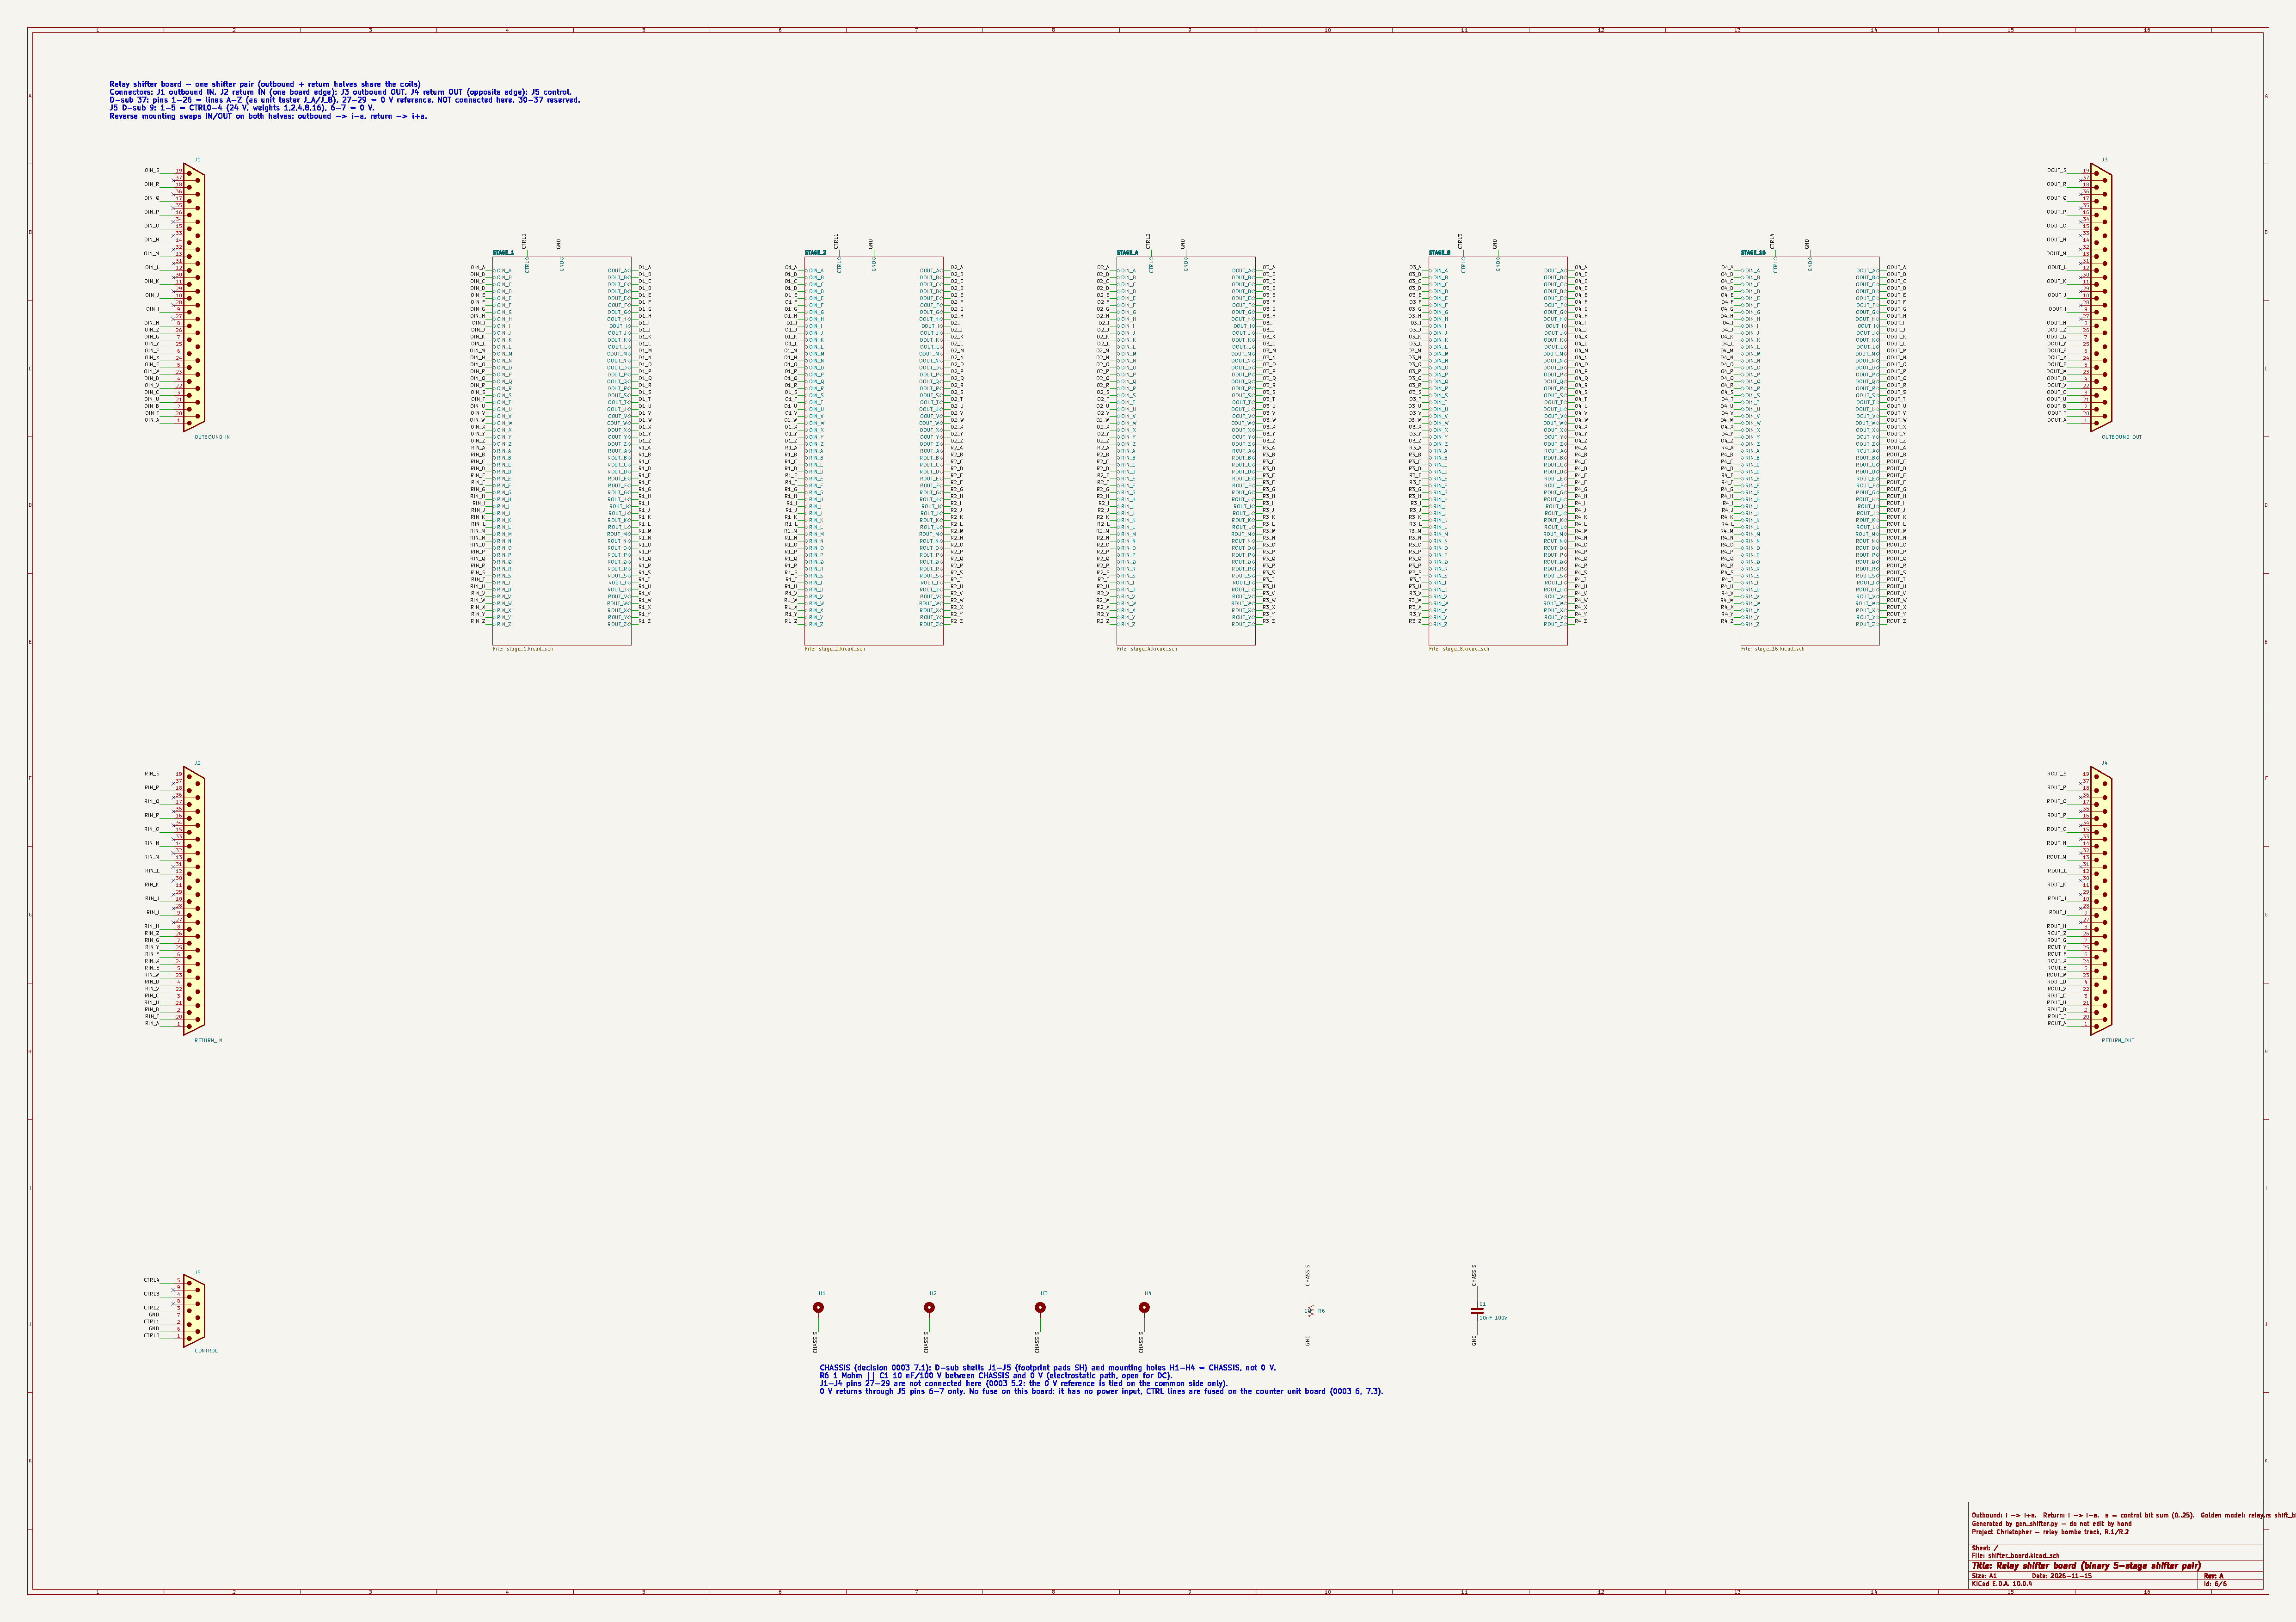
\includepdf[pages=-,pagecommand={\thispagestyle{plain}}]{figures/generated/sch_shifter-board.pdf}}{}

% ======================================================================
\section{릴레이 계수기 보드 (공통, 유닛)}\label{sch:counter-common}

\paragraph{무엇을 하는가.} 시프터의 제어값을 만드는 보드다. 드럼이 도는 대신 릴레이가 위치를 센다
(\ref{sec:hw-relay-counter}절). 세는 값은 다섯이다. $l$(빠른 자리), $m$(가운데 자리), 그리고 시프터에 바로 줄 수
있도록 미리 빼 둔 $a_3 = l - m$, $a_2$, $a_1$이다. 모든 자리가 같은 회로(릴레이 11개)이고 출력은 0--25의 5비트
이진수로, 시프터 보드의 \code{CTRL} 다섯 선을 그대로 구동한다. 보드는 두 장이다.

\begin{table}[ht]
\centering
\small
\begin{tabularx}{\linewidth}{l>{\raggedright\arraybackslash}Xrr}
\toprule
보드 & 내용 & 릴레이 & 다이오드 \\
\midrule
공통 & $l$, $m$, $a_3$ 세 자리와 자리 사이의 계수 규칙 전부. 뱅크에 한 장 & 33 & 196 \\
유닛 & $a_2$, $a_1$ 두 자리(다이얼로 정하는 시작값)와, 공통 보드의 $a_3$·$l$ 코드를 이 유닛의 시프터로 넘기는
중계 릴레이 10개. 유닛마다 한 장 & 32 & 138 \\
\bottomrule
\end{tabularx}
\end{table}

\paragraph{시트.} 공통 보드는 루트(커넥터와 자리 사이의 규칙 배선)와 자리 시트 석 장(\code{common\_pl},
\code{common\_pm}, \code{common\_a3})이다. 유닛 보드는 루트, 자리 시트 두 장(\code{unit\_a2}, \code{unit\_a1}), 중계
시트 한 장(\code{unit\_buf})이다. 자리 시트 다섯 장은 같은 회로다.

\paragraph{한 자리: 주종 쌍.} 비트마다 릴레이가 둘 있다. \emph{종(slave)}은 값을 갖고 그 접점이 출력을 낸다.
\emph{주(master)}는 평소에 종의 \emph{반대값}을 따라가고 있다. 한 자리를 1 올리는 일은 ``뒤집혀야 하는 비트의
종이 주의 값을 받는다''로 끝난다. 뒤집는 것이므로 새 값은 옛 값의 반대, 곧 주가 이미 갖고 있는 값이다.

왜 릴레이를 둘씩 쓰는가. 릴레이 하나로 뒤집으려 하면 그 릴레이의 접점이 자기 코일의 길을 바꾸므로, 펄스가
조금만 길어도 다시 뒤집힌다. 주가 다음 값을 미리 들고 있고 클럭 동안에는 변하지 않으면, 펄스의 길이와 무관하게
한 번만 넘어간다. 클럭은 두 상이다. 평상시(\code{NCK})에는 주가 종을 거울처럼 따라가고, 확정 펄스(\code{CK})
동안에는 주가 스스로를 붙잡고 종이 주의 값을 받는다. 두 상은 전환 접점 하나에서 나오므로 함께 켜지지 않는다.

\paragraph{올림 사슬.} 이진수에 1을 더하면 아래쪽의 1이 연달아 0이 되고 처음 만나는 0이 1이 된다. 곧 비트
$i$가 뒤집히는 조건은 ``아래 비트가 모두 1''이다. 이것을 주 릴레이의 접점을 직렬로 이은 사슬로 만든다.
증가 신호가 비트 0에서 들어가 주가 0인(= 종이 1인) 비트를 지나 위로 올라가고, 주가 1인 비트에서 멈춘다.
사슬이 닿은 비트가 뒤집히는 비트다. 주는 클럭 동안 변하지 않으므로 사슬은 접점만 지나갈 뿐 릴레이의 동작을
기다리지 않는다. 다섯 비트가 같은 순간에 넘어간다. 사슬이 닿지 않은 비트는 정지 레일로 제 값을 유지한다.
정지 레일은 ``사슬이 이 비트에 닿지 않았다''를 다이오드로 모아 만든 것이다.

\paragraph{25 다음은 0.} 5비트는 31까지 셀 수 있지만 자리는 26진이다. 값이 25(\code{11001})일 때에만 꺼지는
릴레이 하나(KW, 코일은 ``비트 0, 3, 4 가운데 하나라도 0''의 다이오드 합)가 비트 1과 2의 거울 길을 끊는다.
그러면 25에서 주는 \code{00110}이 아니라 \code{00000}이 된다. 주가 모두 0이면 사슬이 끝까지 올라가므로 다섯
비트가 모두 주의 값 0을 받고, 사슬의 끝이 곧 다음 자리로 가는 올림이다. 26이라는 중간값이 나타나지 않고,
따로 지우는 회로도 없다. 한 자리는 종 5, 주 5, KW 1로 릴레이 11개다.

\paragraph{자리 사이의 규칙.} $m$은 $l$이 25에서 0으로 넘어갈 때 오르고, $a_3 = l - m$은 매번 오르되 그때만
쉰다. $a_2$와 $a_1$도 같은 식의 규칙이다. 이 규칙은 앞 자리의 올림 레일과 ``25가 아님'' 레일을 다음 자리의
증가·정지 레일에 잇는 것으로 끝나며 모두 공통 보드에 있다. 유닛 보드에는 규칙이 없다. 레일 넷과 코드 열 선을
받아 세기만 하고, 시작값만 유닛마다 다이얼로 정한다($a_1 = k$, $a_2 = -k$. $k$는 그 유닛의 크립 오프셋).
규칙 신호가 모두 주의 값에서 나오므로 같은 클럭에서 종이 바뀌어도 흔들리지 않고, 자리 사이에 순서가 없다.

\paragraph{원위치.} 두 상을 모두 꺼서 릴레이를 전부 놓고, 적재 신호(\code{LOAD})로 종에 시작값을 넣은 다음,
평상시 상을 올리고 나서 적재 신호를 내린다. 순서가 바뀌어 틈이 생기면 넣은 값이 지워진다. 전원을 켠 직후의
임의 상태에서도 이 순서가 맞는 값을 만든다.

\paragraph{커넥터와 전류.} 공통 보드는 클럭(D-sub 9)과 유닛 버스(D-sub 25: 레일 넷, $l$과 $a_3$의 코드 열 선,
적재)를, 유닛 보드는 버스, 다이얼(D-sub 15), 시프터 넉 장으로 가는 제어 커넥터 넷(D-sub 9)을 갖는다. 한 자리는
늘 여섯쯤의 릴레이가 붙어 있어 1.1--1.5~W다. $a_1$과 $a_2$는 종의 접점이 시프터 한 단(약 0.2~A)을 바로 구동하고,
$a_3$과 $l$은 유닛마다 중계 릴레이를 거친다. 공통 보드의 접점 하나가 모든 유닛의 시프터를 떠맡지 않게 하려는
것이다.

\paragraph{확인.} ERC는 두 보드 모두 위반 0건이다. 검증 스크립트는 넷리스트만 읽어 접점 수준으로 풀고, 자기
유지가 있으므로 릴레이의 상태를 이어 가며 클럭을 넣는다. 기준은 \code{relay.rs}의 계수기를 옮긴 것이다.

\begin{itemize}
\item 자리 하나: 시작값 0--25 각각에서 증가와 정지를 섞은 60걸음(모두 1,560걸음)의 값과 올림.
\item 원위치: 크립 오프셋 26가지 전부, 릴레이의 처음 상태를 무작위로 두고. 순서를 바꾼 네 가지를 150번.
\item 전체 구동: 공통 한 장과 유닛 석 장을 한 시스템으로 묶어 17,576 클럭. 오프셋 0--25를 모두 거쳤다. 클럭마다
두 시점에서 모든 유닛의 제어값 넷과 내부 자리 다섯의 주·종 값을 기준과 견주었다. 불일치 0.
\item 경주: 바뀔 릴레이를 무작위 순서로 하나씩 넘기는 방식으로 17,576 클럭을 다시 돌렸다. 통과. 릴레이마다
빠르기가 달라도 결과가 같다는 뜻이다.
\item 음성 시험: 버스선, 접점, 다이오드의 방향, 다이얼의 비트, 커넥터 핀을 바꾼 14가지를 모두 잡았다.
\end{itemize}

이 시뮬레이션은 연결과 순서를 본다. 릴레이의 동작 시간과 코일 전압은 보지 않는다. 가장 깊은 길은 다이오드
넷을 지나므로 코일 전압이 1.2--1.6~V 깎인다. 그래서 보드의 전원 단자에서 23.0~V 이상을 요구한다.

\paragraph{고칠 곳.} 전원을 버스 커넥터로 받게 되어 있으나 유닛 하나가 최악 2.5--3.6~A를 쓰므로 보드마다 전원
단자를 따로 둔다. 뱅크의 위치(\code{POS})를 내보내는 커넥터가 없고, 느린 자리 $r$을 세는 자리도 없다(유닛의
$a_1$은 $r + k$다). 공통 보드에 자리 하나를 더한다.

\IfFileExists{figures/generated/sch_counter-common.pdf}{%
  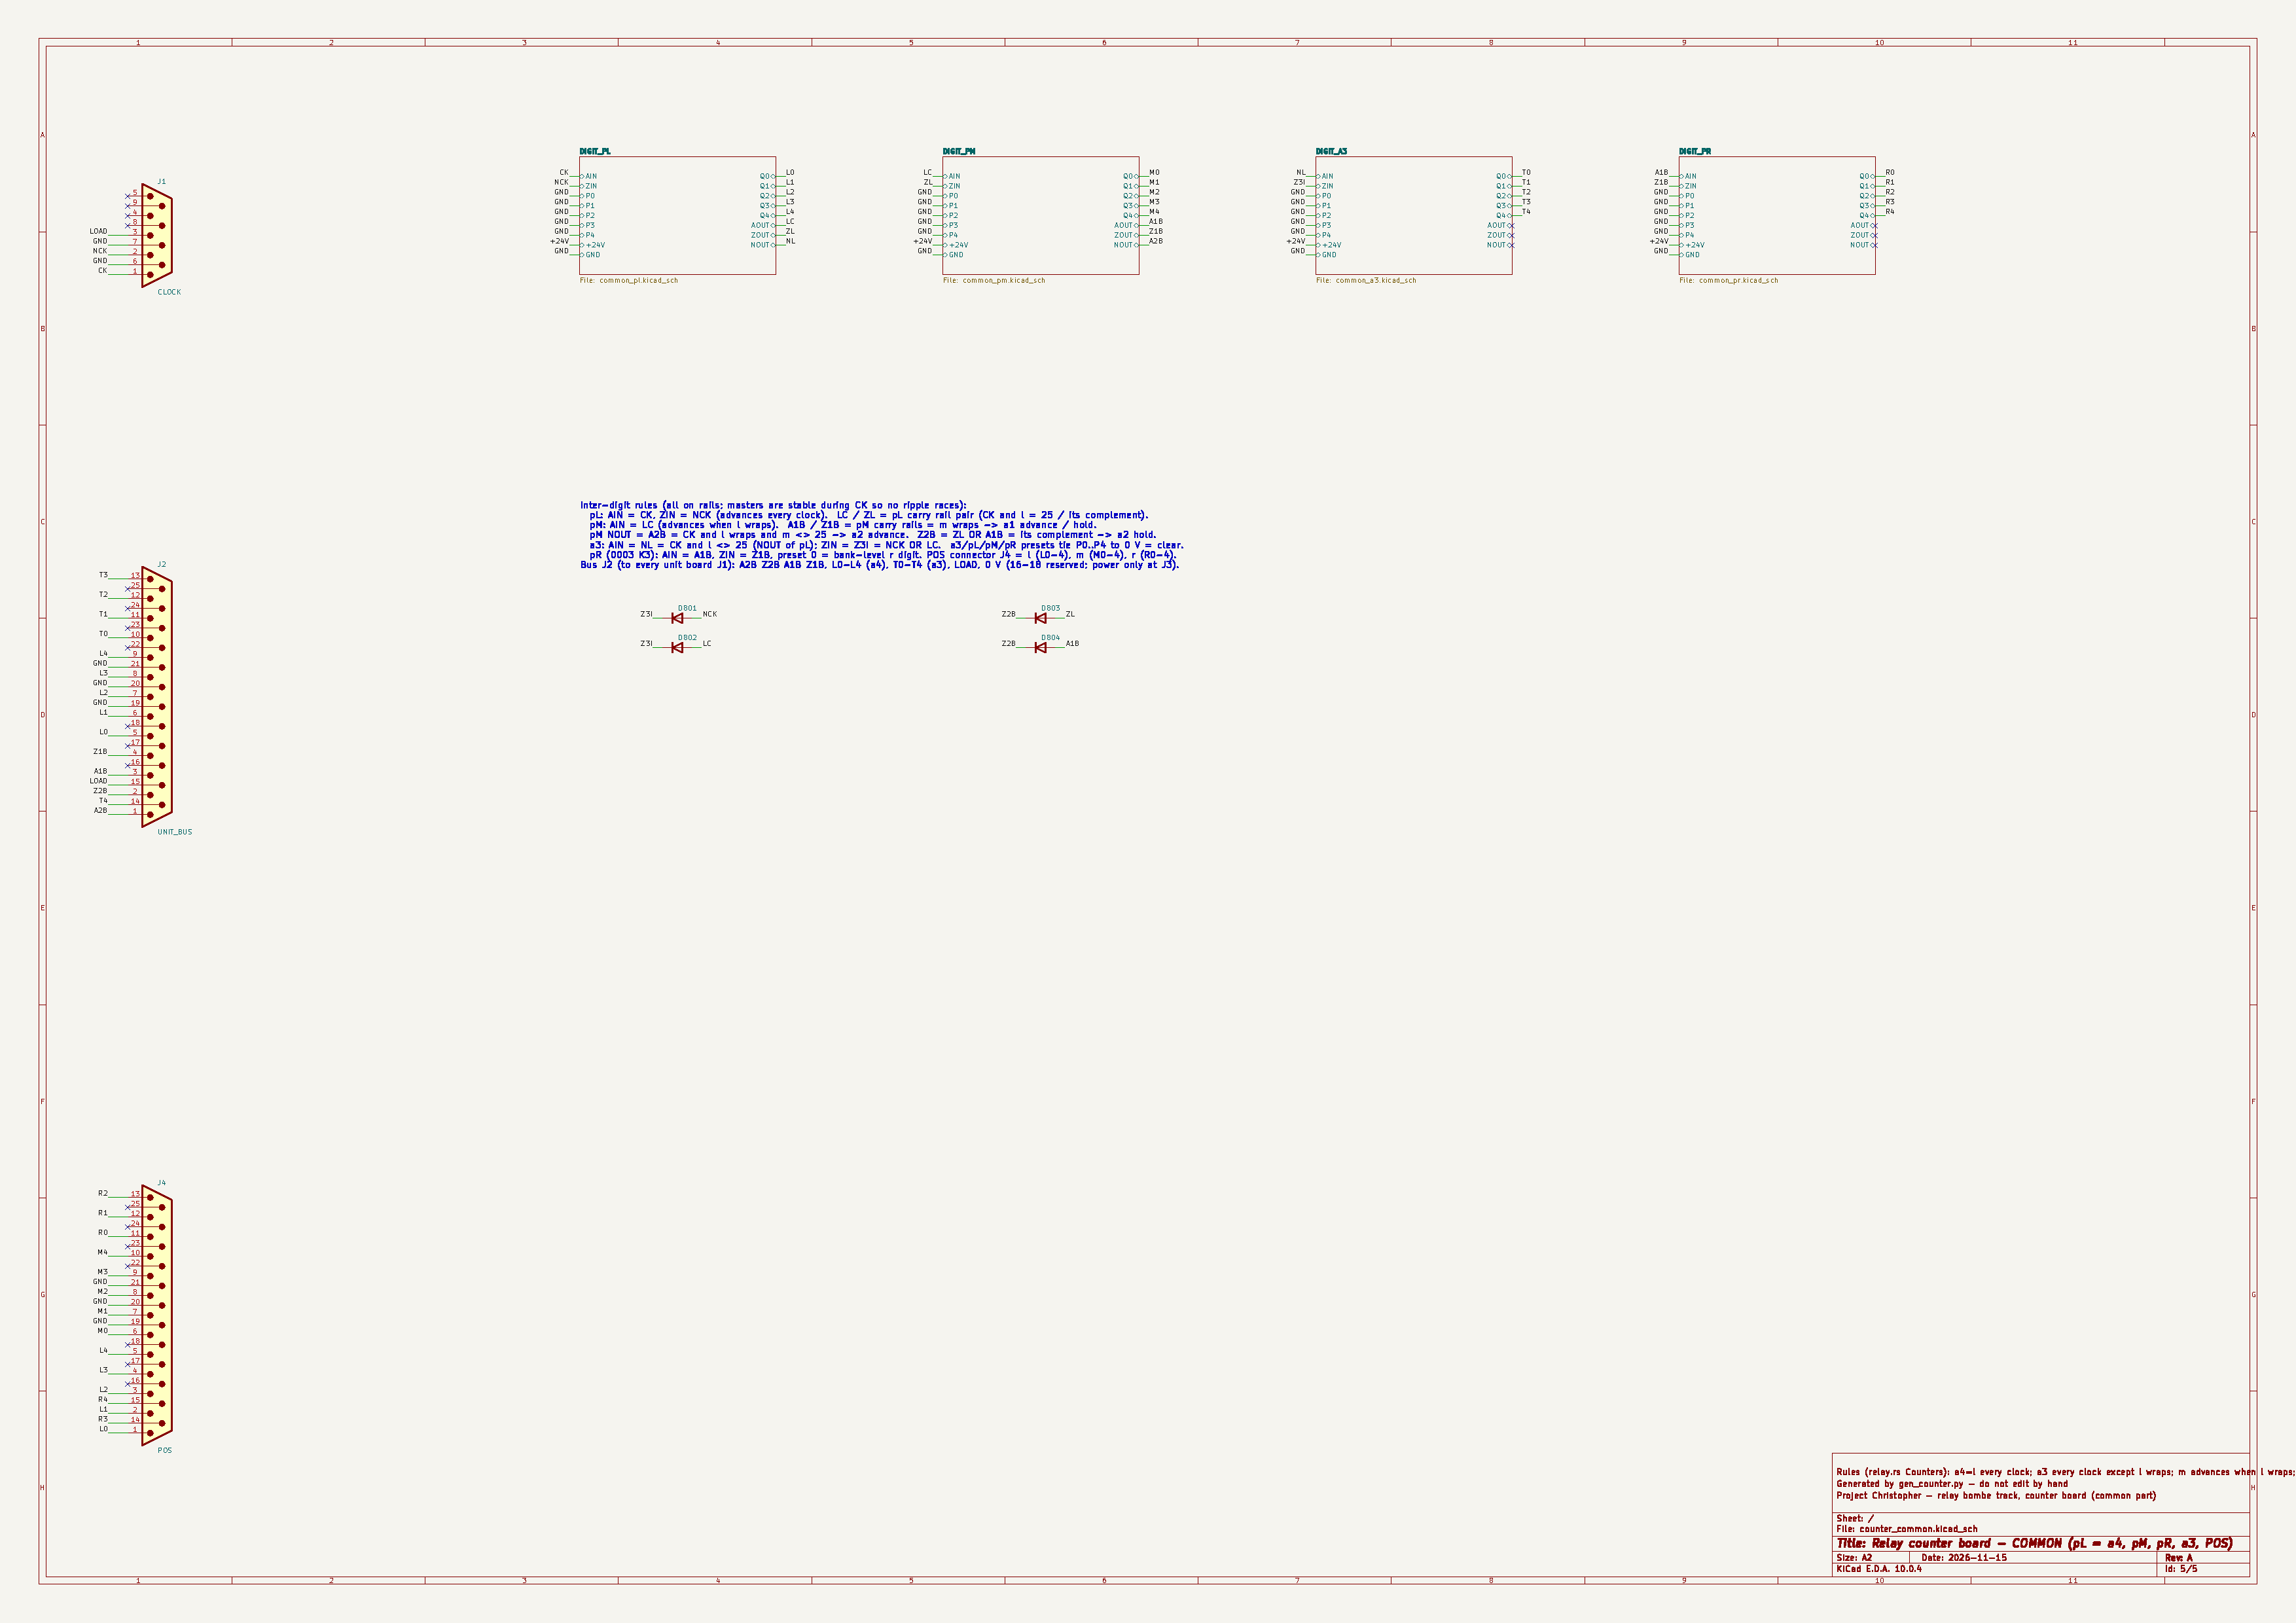
\includepdf[pages=-,pagecommand={\thispagestyle{plain}}]{figures/generated/sch_counter-common.pdf}}{}
\IfFileExists{figures/generated/sch_counter-unit.pdf}{%
  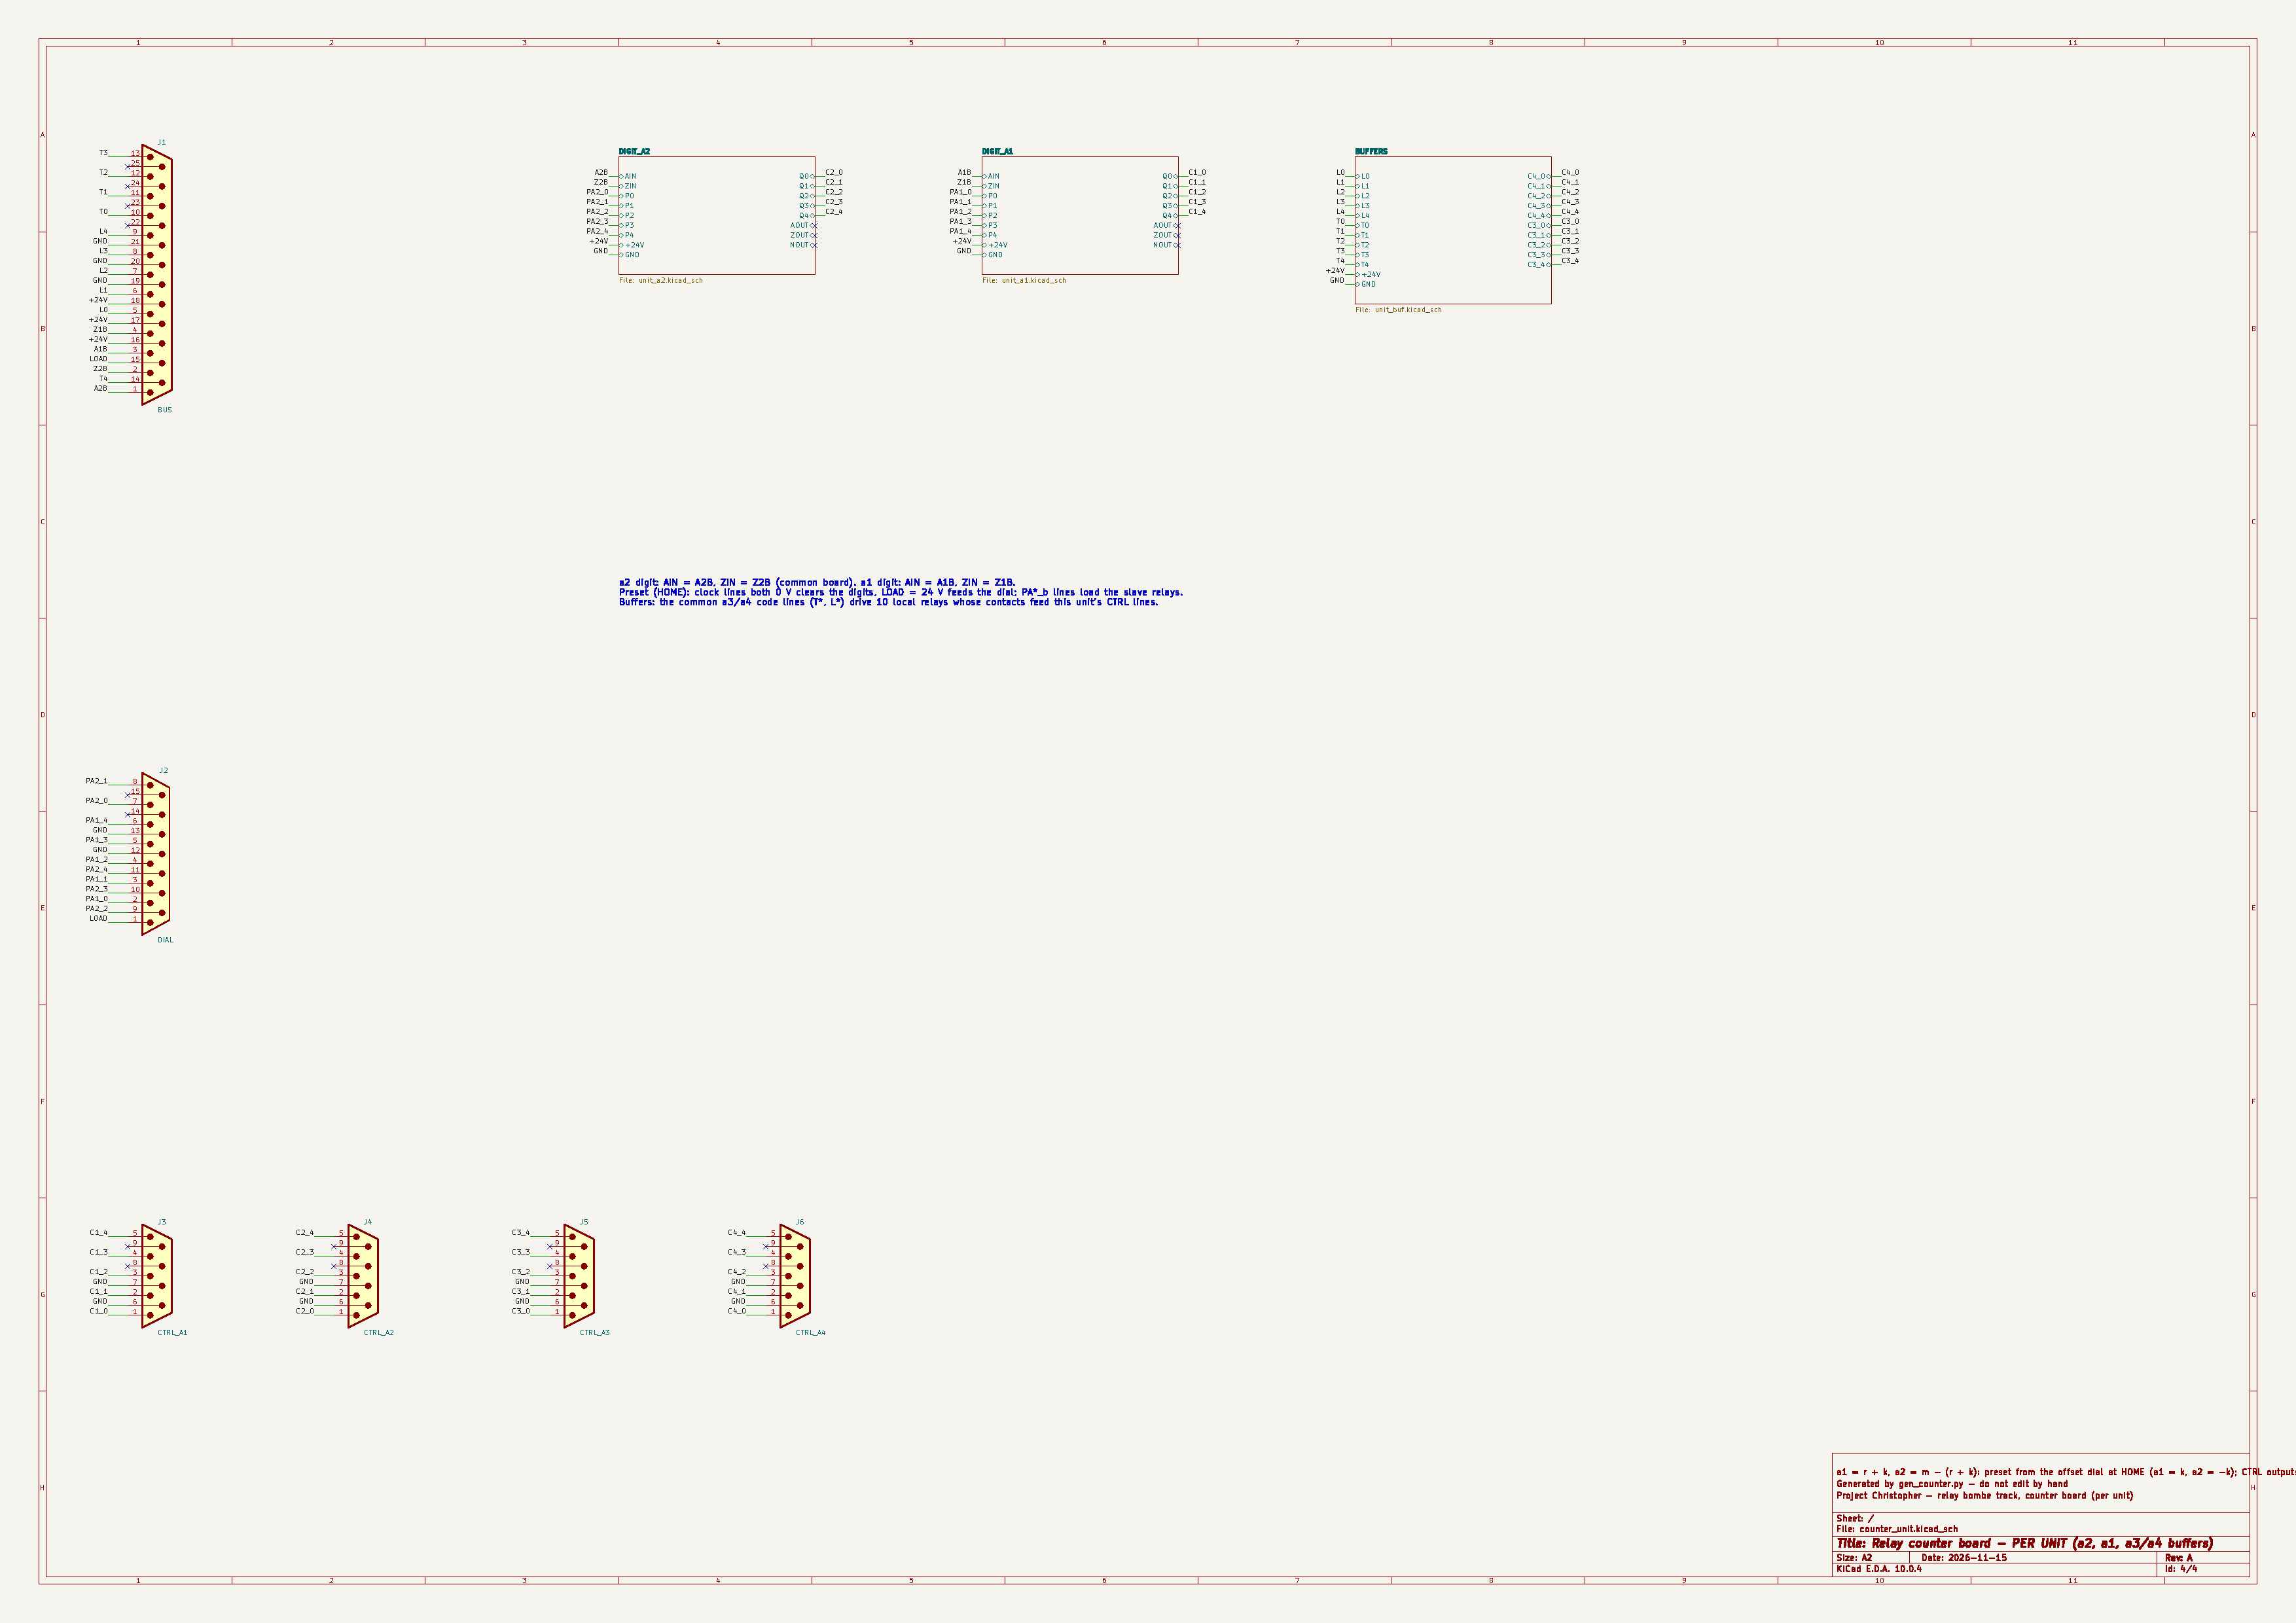
\includepdf[pages=-,pagecommand={\thispagestyle{plain}}]{figures/generated/sch_counter-unit.pdf}}{}

% ======================================================================
\section{테스트 레지스터 보드}\label{sch:test-register}

\paragraph{무엇을 하는가.} 공통부의 한가운데다. 입력 케이블의 26선을 받아 ``전부 통전되지는 않았는가''를
릴레이로 판정하고, 정지이면 뱅크를 세우고 그 순간의 26선을 붙들어 보여 준다. 원리와 그림은
\ref{sec:hw-register}절(그림~\ref{fig:hw-register})에 있다. 이 절은 그 회로가 보드에서 어떤 부품이 되었는지를
적는다. 신호 릴레이 34개, 표시를 구동하는 MOSFET 28개, 부품 258개다.

\paragraph{시트.} 두 장이다. \code{sense\_lanes}에는 같은 모양의 레인 26개가 있다. 레인 하나가 글자 하나다: 선에서
오는 차단 다이오드, 감지 릴레이(접점 한 벌은 자기 유지, 한 벌은 사슬), 코일 다이오드, 표시 구동(분압 저항 둘과
MOSFET), 보드 위의 표시등. 루트 시트에는 나머지가 있다: 타이밍 릴레이 셋, 통과 릴레이, 정지 릴레이 셋, 해제
릴레이, 정지 중에만 표시 쪽 0~V를 잇는 MOSFET, 커넥터, 전원의 퓨즈 둘.

\paragraph{한 위치에서 일어나는 일.} 그림~\ref{fig:hw-register}의 번호로 적는다.

\begin{enumerate}
\item \textbf{감지}(0--6~ms). \code{STROBE} 릴레이의 접점이 닫혀 시험 전압이 나간다. 통전된 선의 레인에서 전류가
다이오드를 지나 감지 릴레이를 붙이고, 붙은 릴레이는 유지 버스 $H$에서 스스로를 유지한다(그림의 (1)).
\item \textbf{정착}(6--12~ms). 26개가 모두 붙었으면 사슬이 이어져 통과 릴레이가 붙는다((3)).
\item \textbf{판정}(12--19~ms). \code{JUDGE} 릴레이의 접점이 닫힌다. 통과 릴레이가 놓여 있으면 그 b접점을 지나
정지 릴레이 셋이 붙어 자기 유지에 들어간다((4)). 정지 릴레이는 유지 버스를 우회해 감지 릴레이를 붙들고,
시험 전압을 끊고, \code{RUN}을 끊고, 표시 쪽 0~V를 이어 램프를 켠다.
\item \textbf{복귀}(21--33~ms). \code{CLEAR} 릴레이의 b접점이 열려 $H$가 끊기고 감지 릴레이와 통과 릴레이가
놓인다((2)). 정지 중이면 우회 때문에 아무것도 놓이지 않는다.
\end{enumerate}

\paragraph{보드로 옮기며 고친 네 곳.} 넷리스트를 릴레이의 동작·복귀 시간을 넣어 시뮬레이션하자 계산으로 정한
회로의 네 곳이 틀린 것으로 드러났다. 사슬을 $+24$~V가 아니라 $H$에서 먹일 것(통과 릴레이가 늦게 놓여 다음
위치의 정지를 놓친다), 통과 릴레이의 유지 접점에 직렬 다이오드를 넣을 것($H$가 거꾸로 살아난다), 정지 잠금과
정지 릴레이의 자기 유지를 $HSUP$에서 받을 것(해제 하나로 다 풀리게), 해제 릴레이를 둘 것(재출발 때 레지스터를
비운다). 이유는 \ref{sec:hw-register}절에 풀어 적었다.

\paragraph{왜 표시는 접점이 아니라 MOSFET인가.} 표시용 큰 릴레이 26개의 코일 전류는 합해 약 1~A다. 감지
릴레이의 접점으로 구동하면 이 전류가 유지 버스와 유지 접점을 지난다. 그래서 감지 릴레이의 코일 마디 전압을
분압해 MOSFET의 게이트에 주고, 표시 전류는 표시 커넥터의 $+24$~V(따로 2~A 퓨즈)에서 표시 릴레이와 MOSFET을
지나 0~V로 흐르게 했다. 판정의 길에는 전자 부품이 없다.

\paragraph{커넥터.} J1이 26선 입력, J2가 뱅크 제어(1번 \code{STROBE}, 2번 \code{RUN}, 3번 \code{STOPPED}, 34번
\code{JUDGE}, 35번 \code{CLEAR}, 36번 \code{STOP\_LATCH}), J3이 표시(1--26번 글자, 27번 정지 램프, 열린 드레인),
J4가 24~V 입력, J5가 시험 전압 선, J6이 앞면 패널(시작, 해제)이다.

\paragraph{전류.} 코일 하나에 약 8~mA이므로 26선이 모두 붙고 나머지 릴레이까지 더한 최악이 약 0.3~A, 정지 중의
보드 위 표시등이 0.17~A다. 논리 쪽 퓨즈는 유지 전류 1.1~A다.

\paragraph{확인.} ERC는 위반 0건이다. 검증 스크립트는 넷리스트에서 접점, 다이오드, MOSFET을 풀어 시간에 따라
사건을 진행시키고, 뱅크의 신호와 메뉴 배선망을 흉내 낸다. 배선망은 \code{STROBE} 동안에는 통전된 선들을 시험
선에 잇고 그 밖의 시간에는 엉뚱한 선들을 이어, 유지 전압이 배선망으로 새는지도 함께 본다.

\begin{itemize}
\item 438개의 위치 주기, 정지 176회. 26선이 전부 통전된 위치에서 거짓 정지 0.
\item 사례: 26선 전부, 25선 26가지, 1선 26가지, 0선, 무작위 부분집합 120, 정지·정지 중 주행·해제를 섞은 순서 12,
릴레이가 모두 가장 느리거나 가장 빠른 경우.
\item 폭이 비정상인 \code{STROBE}(2--8~ms)와 무작위 릴레이 시간 60번: 놓친 정지 0, 거짓 정지 6(안전한 쪽).
\item 릴레이가 가장 느릴 때의 최소 폭: \code{STROBE} 5~ms, \code{JUDGE} 5~ms, \code{CLEAR} 10~ms.
\item 음성 시험 18가지(다이오드의 방향, 접점의 종류, 각 릴레이의 기능, 신호와 선의 뒤바뀜)를 모두 잡았다.
\end{itemize}

접점의 튐과 코일 전압의 강하는 모델에 없다. 시제품에서 잰다.

\paragraph{고칠 곳.} 타이밍 릴레이의 코일은 빨리 놓이도록 다이오드와 제너로 클램프했는데, 코일이 커넥터의 핀에
바로 붙어 있어 신호가 꺼질 때 핀이 약 $-31$~V까지 내려간다. 핀과 코일 사이에 다이오드를 하나씩 넣어 이 전압이
뱅크로 나가지 않게 한다. 그 밖에 패널 단자에 Home 버튼과 비상 정지의 자리, 커넥터 껍데기의 섀시 접지, 전원의
역극성 보호를 더한다.

\IfFileExists{figures/generated/sch_test-register.pdf}{%
  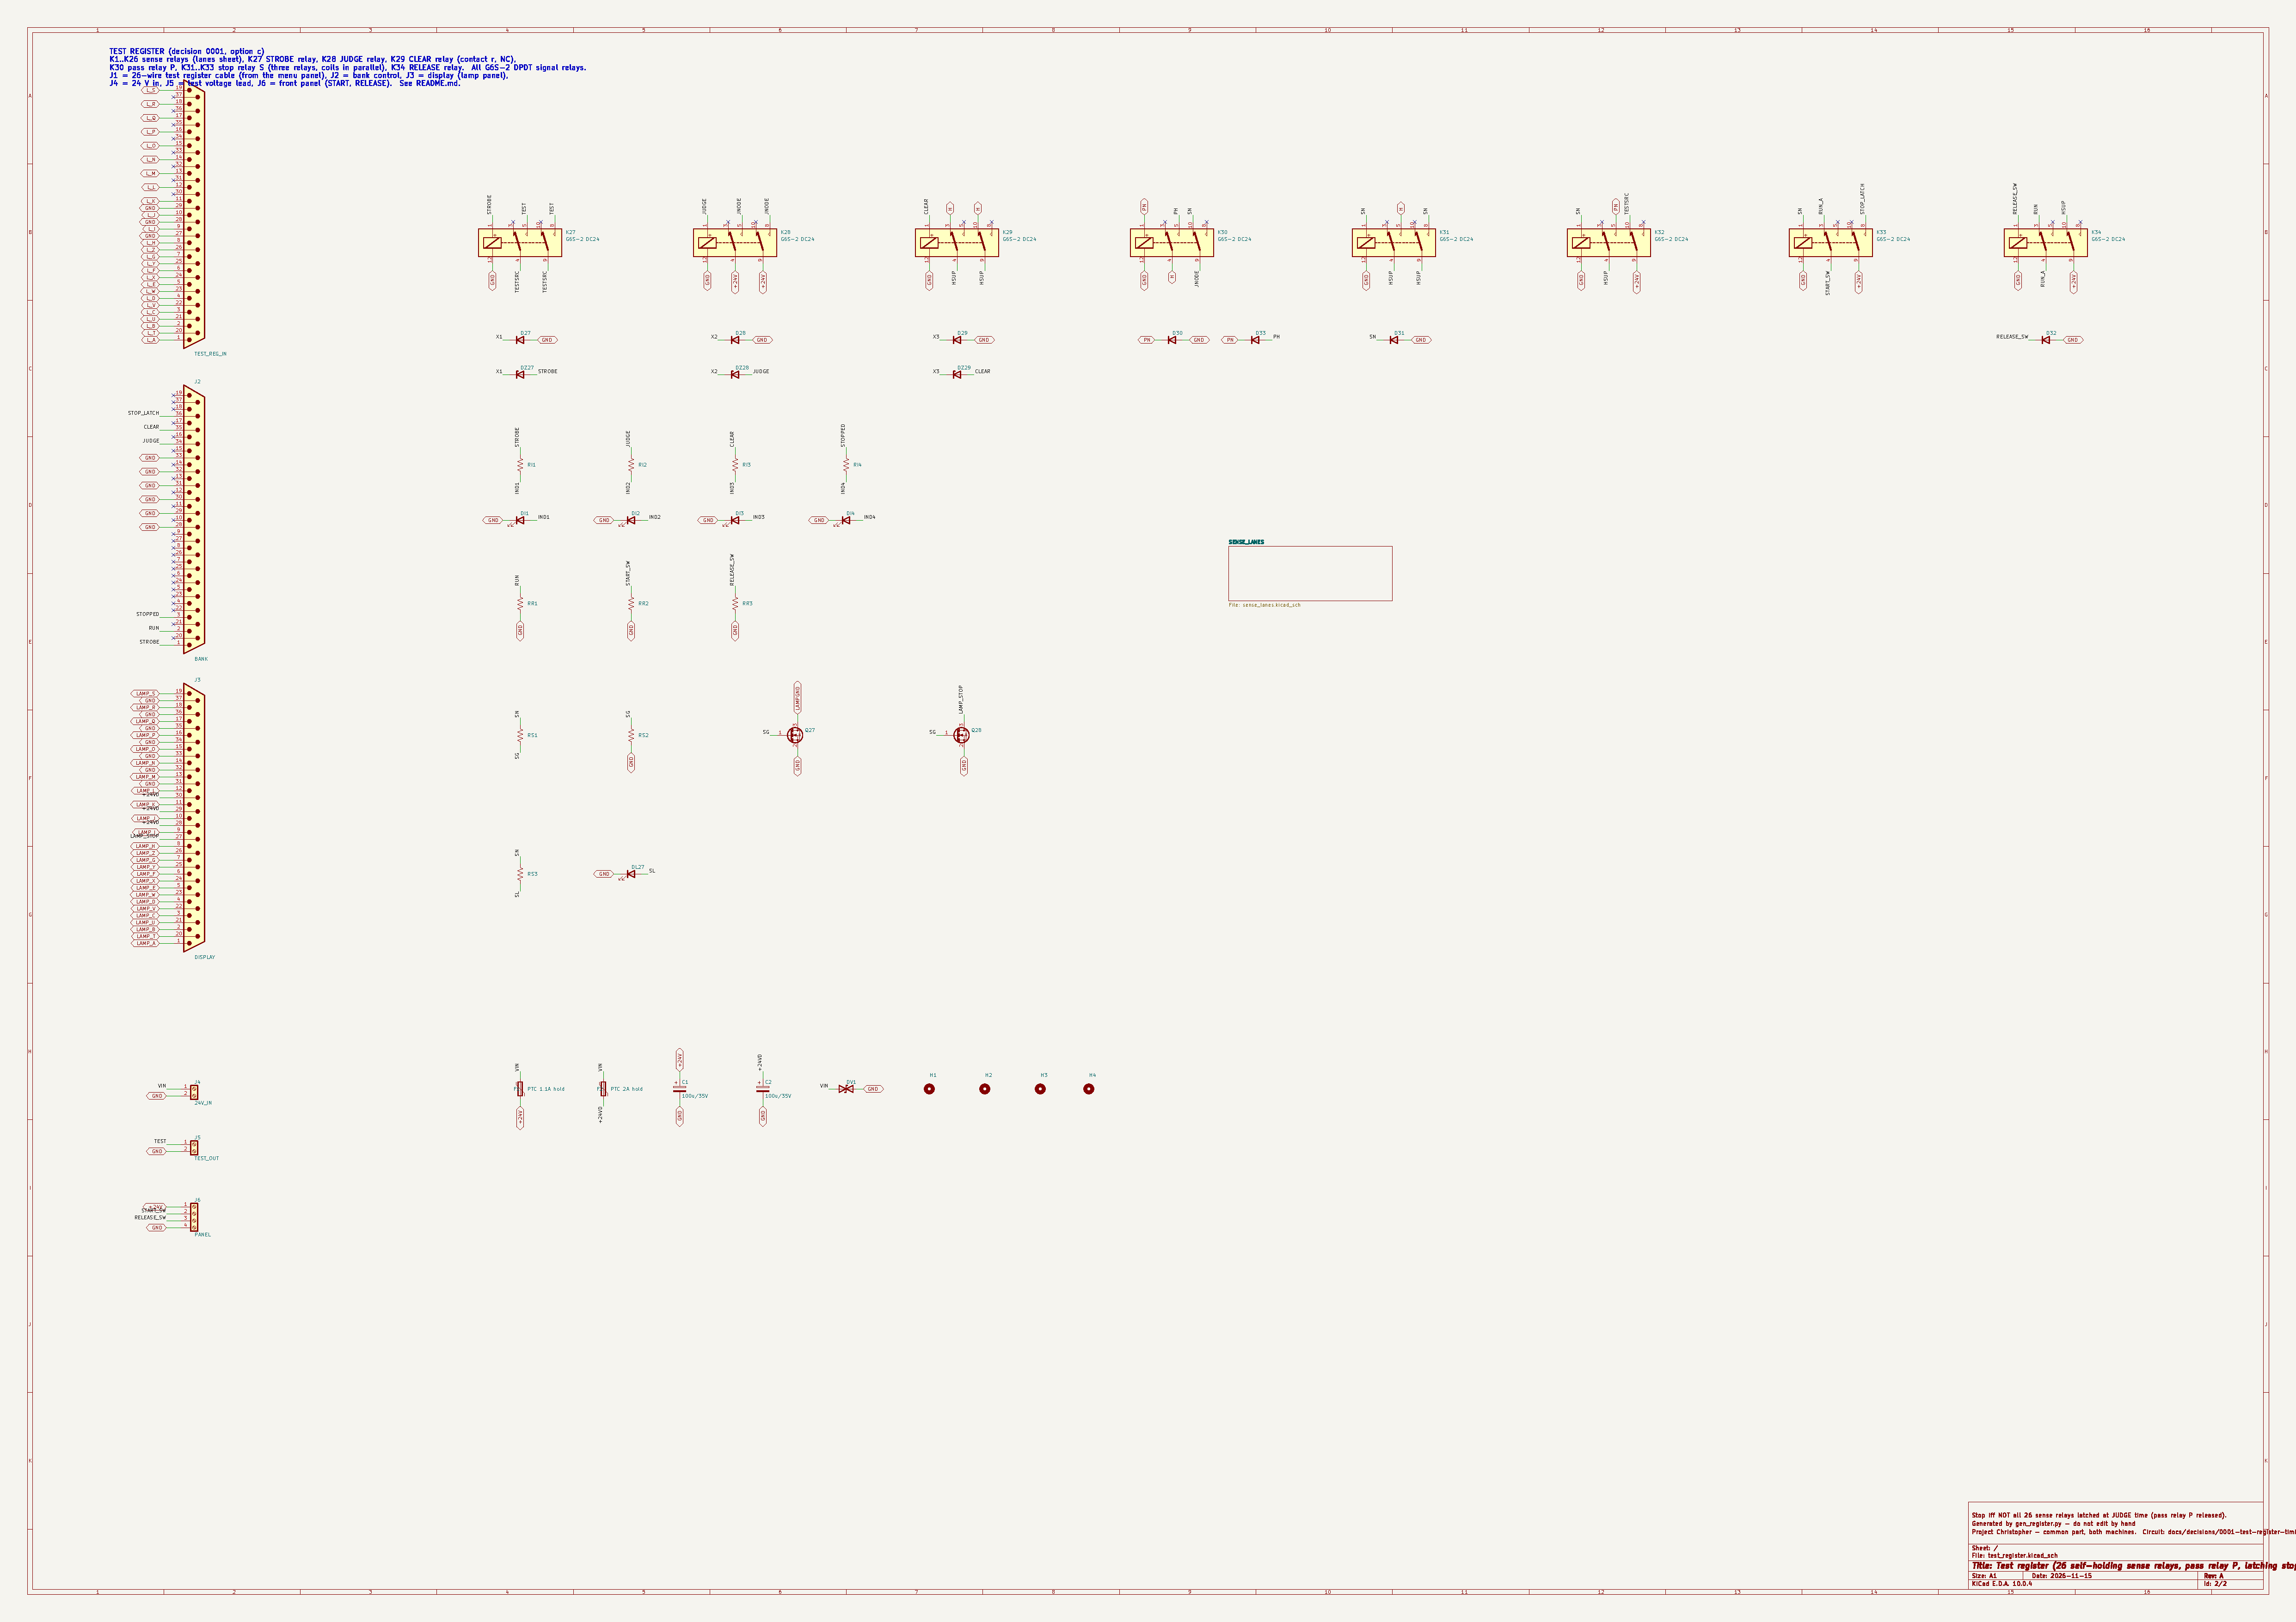
\includepdf[pages=-,pagecommand={\thispagestyle{plain}}]{figures/generated/sch_test-register.pdf}}{}

% ======================================================================
\section{스크램블러 단위 시험기}\label{sch:unit-tester}

\paragraph{무엇을 하는가.} 스크램블러 하나(또는 드럼 기판 한 장, 시프터 보드 한 장)를 꽂으면 26선과 26선
사이의 연결을 모두 읽어 소프트웨어 기준 모델과 견주는 장치다. 연결은 위치마다 $26 \times 26$개이고 위치가
17,576개이므로 손으로는 할 수 없다. 대상은 전원이 없는 수동 소자로 보고, 한쪽 26선을 A, 반대쪽 26선을 B라
부른다. 쓰는 순서는 \ref{sec:app-procedure}절에 있다.

\paragraph{한 노드의 구동과 감지.} 52선 하나하나가 같은 회로를 갖는다(그림~\ref{fig:sch-tester-node}). 구동 쪽은
고측 구동기 한 채널이 24~V를 1~k$\Omega$을 거쳐 선에 건다. 감지 쪽은 같은 선에서 2.2~k$\Omega$과 광커플러의
발광부를 거쳐 0~V로 간다. 한 선을 구동하면 그 선과 대상물 안에서 이어진 선의 광커플러가 켜진다. 한 번에 한
선씩 26번(또는 52번) 구동하고 그때마다 52선을 읽으면 연결의 표 전체가 나온다.

왜 24~V로 시험하는가. 접점 표면의 얇은 산화막은 낮은 전압과 작은 전류로는 뚫리지 않는다. 3.3~V로 읽으면
기계에서는 멀쩡히 통하는 접점을 끊어진 것으로 읽을 수 있다. 전시 기계와 같은 전압과 비슷한 전류(약 7~mA)로
읽어야 같은 답이 나온다. 1~k$\Omega$은 어떤 선이 0~V에 닿아도 전류를 24~mA로 묶는다.

\begin{figure}[ht]
\centering
\begin{tikzpicture}[x=1cm,y=1cm]
  \node[blkn] (pico) at (0,0) {Pico};
  \node[blkn] (iso) at (2.3,0.7) {절연기};
  \node[blkb] (sr) at (4.5,0.7) {74HC595};
  \node[blkb] (drv) at (6.9,0.7) {고측 구동기};
  \node[blk] (r1) at (9.2,0.7) {1 k$\Omega$};
  \node[circle,fill,inner sep=1.3pt] (n) at (10.8,0.7) {};
  \node[font=\footnotesize,anchor=west] at (11.0,0.7) {노드 $\to$ 커넥터의 선};
  \node[blk] (r2) at (9.2,-0.7) {2.2 k$\Omega$};
  \node[blko] (opt) at (6.9,-0.7) {광커플러};
  \node[blkb] (si) at (4.5,-0.7) {74HC165};
  \draw[->] (pico) |- (iso);
  \draw[->] (iso) -- (sr);
  \draw[->] (sr) -- (drv);
  \draw[->] (drv) -- (r1);
  \draw (r1) -- (n);
  \draw[->] (n) |- (r2);
  \draw[->] (r2) -- (opt);
  \draw[->] (opt) -- (si);
  \draw[->] (si) -| (pico);
  \draw[dashed,cred] (1.2,-1.5) -- (1.2,1.5);
  \draw[dashed,cred] (1.2,-0.05) -- (5.8,-0.05) -- (5.8,-1.5);
  \node[note,text=cred] at (0,1.3) {USB 쪽 (3.3 V)};
  \node[note,text=cred] at (8.0,1.5) {현장 쪽 (24 V)};
\end{tikzpicture}
\caption{단위 시험기의 한 노드. 위가 구동, 아래가 감지다. 점선이 절연 장벽이다. 구동은 디지털 절연기에서, 감지는
광커플러에서 장벽을 건넌다. 같은 회로가 52개 있다.}
\label{fig:sch-tester-node}
\end{figure}

\paragraph{절연.} 보드는 두 영역이다. 현장 쪽(24~V 어댑터: 구동기, 광커플러의 발광부, 구동용 시프트 레지스터)과
USB 쪽(Pico, 감지용 시프트 레지스터)이다. 현장 쪽의 0~V는 기계의 프레임과 모터 전원으로 이어질 수 있으므로
PC와 직접 닿으면 안 된다. 두 영역을 건너는 부품은 디지털 절연기 둘, \code{STROBE}용 고속 광커플러 하나, 감지
광커플러 열아홉뿐이다. 넷리스트 검사가 ``두 영역의 핀이 한 넷에 섞이지 않는다, 수동 소자가 두 영역을 잇지
않는다''를 확인한다(현장 쪽 넷 313개, USB 쪽 132개, 섞인 넷 0).

\paragraph{시트.} 루트와 하위 시트 14장이다. \code{power}(24~V 입력, 퓨즈, 5~V 강압), \code{mcu}(Pico),
\code{isolation}(절연기 둘과 \code{STROBE} 광커플러), \code{shift\_out}(74HC595 일곱 개), \code{shift\_in}(74HC165 열
개), \code{frontend\_g0}--\code{g6}(노드 여덟 개씩: 구동기 하나, 1~k$\Omega$, 2.2~k$\Omega$, 4채널 광커플러 둘),
\code{aux\_sense}(위치 15선, 뱅크의 상태 신호, 안전 사슬, \code{JUDGE}·\code{CLEAR}), \code{connectors}(D-sub 37 세 개와
저항 측정용 헤더).

\paragraph{뱅크와의 연결.} 세 번째 커넥터는 뱅크 제어 커넥터다. 시험기는 여기서 공통부의 자리에 선다.
\code{RUN}과 \code{HOME}을 내고, \code{STROBE}, 위치, 상태 신호를 읽는다. 대상이 스스로 돌아가는 동안
\code{STROBE}마다 한 번씩 읽으면 위치를 따라가며 시험할 수 있다. 구동기의 입력은 풀다운되어 있고 출력 허가는
풀업이어서, 부팅 중이거나 USB가 빠지면 모든 구동이 꺼진다.

\paragraph{확인.} ERC는 위반 0건이다(루트와 14장). 넷리스트 검사는 1,924가지를 확인했고 실패가 없다. 52노드
각각에서 시프트 레지스터의 비트 $\to$ 구동기 채널 $\to$ 1~k$\Omega$ $\to$ 노드 $\to$ 커넥터의 핀, 같은 노드에서
2.2~k$\Omega$ $\to$ 광커플러 $\to$ 시프트 레지스터의 같은 번호 비트로 이어지는지를 본다. 펌웨어의 핀 지도는 소스에서
읽어 넷리스트와 견준다. 넷 이름 두 쌍을 바꾼 넷리스트는 실패로 잡혔다. 펌웨어와 호스트 프로그램은 가상의
대상물(52노드의 도체 그래프에 결함을 넣은 것)로 시험했다. 실물로는 아직 시험하지 않았다.

\paragraph{고칠 곳.} 커넥터가 소켓이다. 다른 보드와 같은 케이블을 쓰도록 핀으로 바꾼다. \code{RUN}과
\code{HOME} 출력의 직렬 1~k$\Omega$은 뱅크의 입력이 릴레이 코일이면 전압이 모자라므로 자동 복귀 퓨즈로 바꾼다.
안전 사슬은 뱅크가 전원을 주는 고리로 바꾸고, \code{STOP\_LATCH}를 읽는 입력을 더한다.

\IfFileExists{figures/generated/sch_unit-tester.pdf}{%
  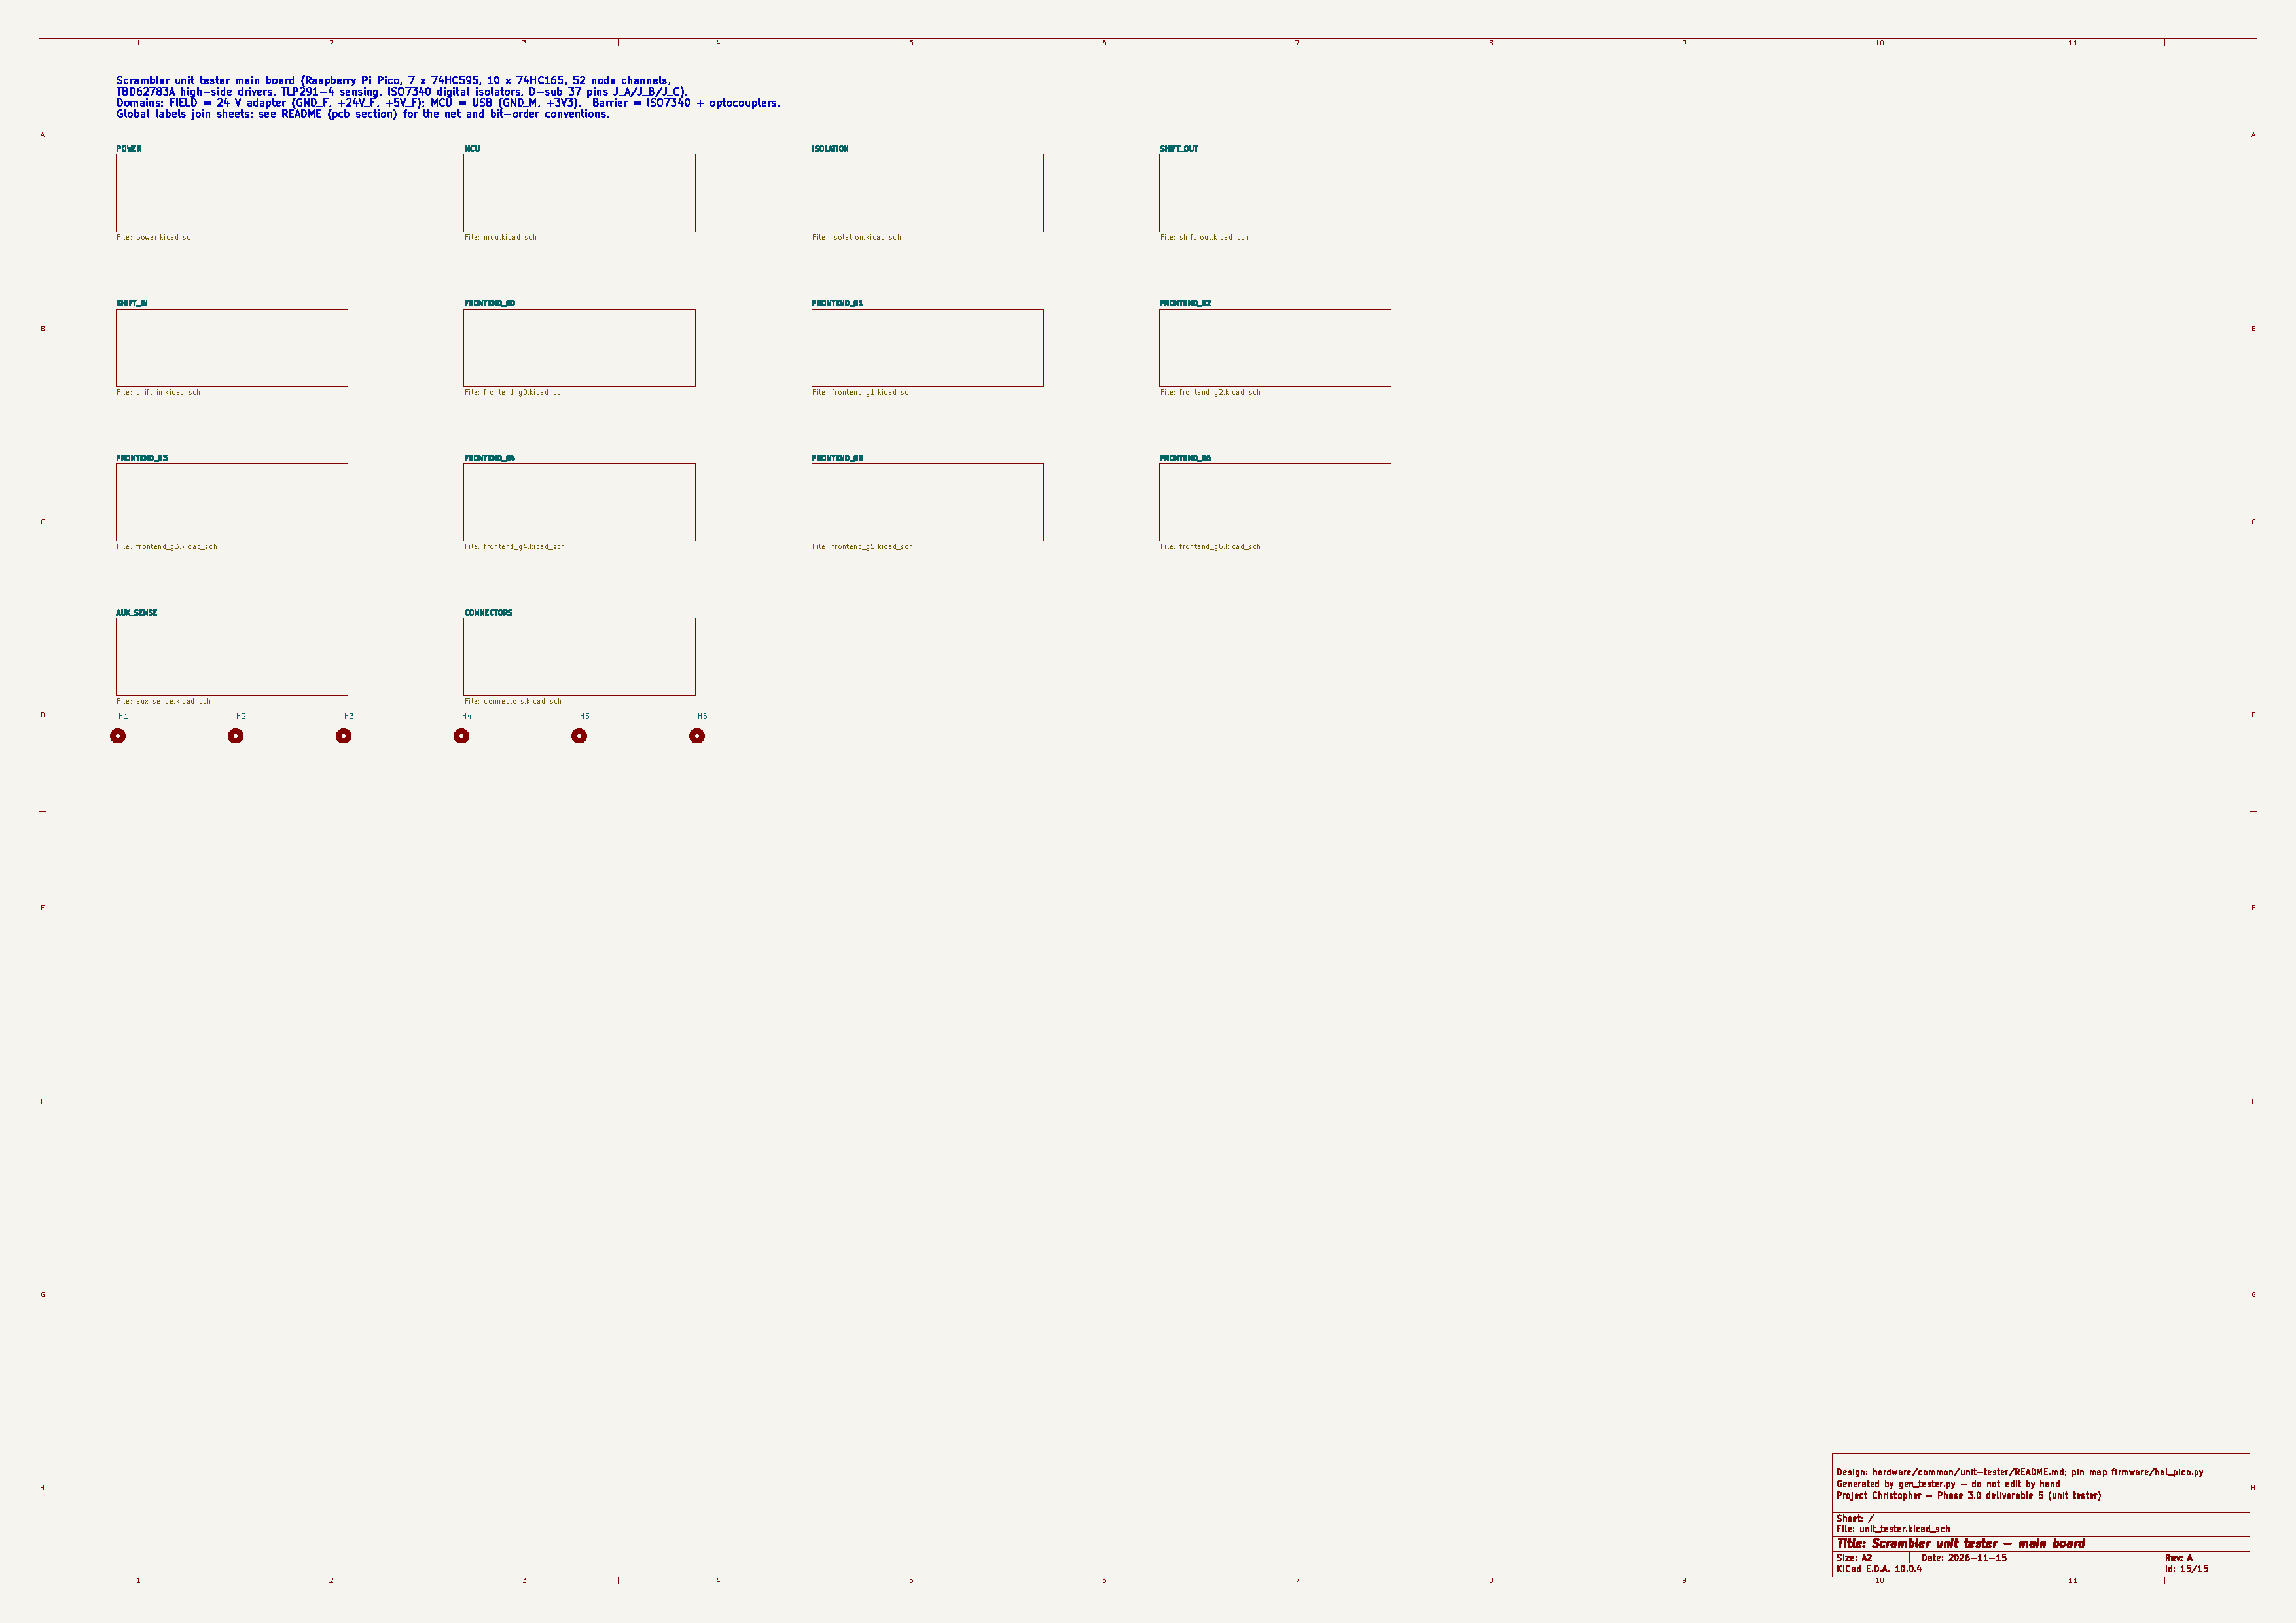
\includepdf[pages=-,pagecommand={\thispagestyle{plain}}]{figures/generated/sch_unit-tester.pdf}}{}

\section{기어식 접점 보드와 열 배선}\label{sch:contact-board}
드럼 한 자리마다 한 장인 접점 보드(Omniball 7845 접점 104개, 반지름 22/29/36/43\,mm의 네 링), 열의 입출력 단자,
반사판 배선 카드(B, C)다. 세 자리와 단자, 반사판 카드가 1:1 리본 여덟 가닥으로 이어져 한 열이 스크램블러 하나가
된다. \code{hardware/gear/contact-board/verify\_column.py}가 보드 파일에서 접점의 링과 위치를 읽어 열 전체를
조립하고, 로터 I--V의 60개 순서 × 17,576 위치 모두(1,054,560가지)에서 입력→출력 연결이 에니그마 스크램블러와
같음을 확인했다. 부정 시험(거울상 보드, 리본 핀 뒤바꿈, 잘못된 반사판 카드, 잘못된 링 등)은 모두 잡힌다.
\IfFileExists{figures/generated/sch_contact-board.pdf}{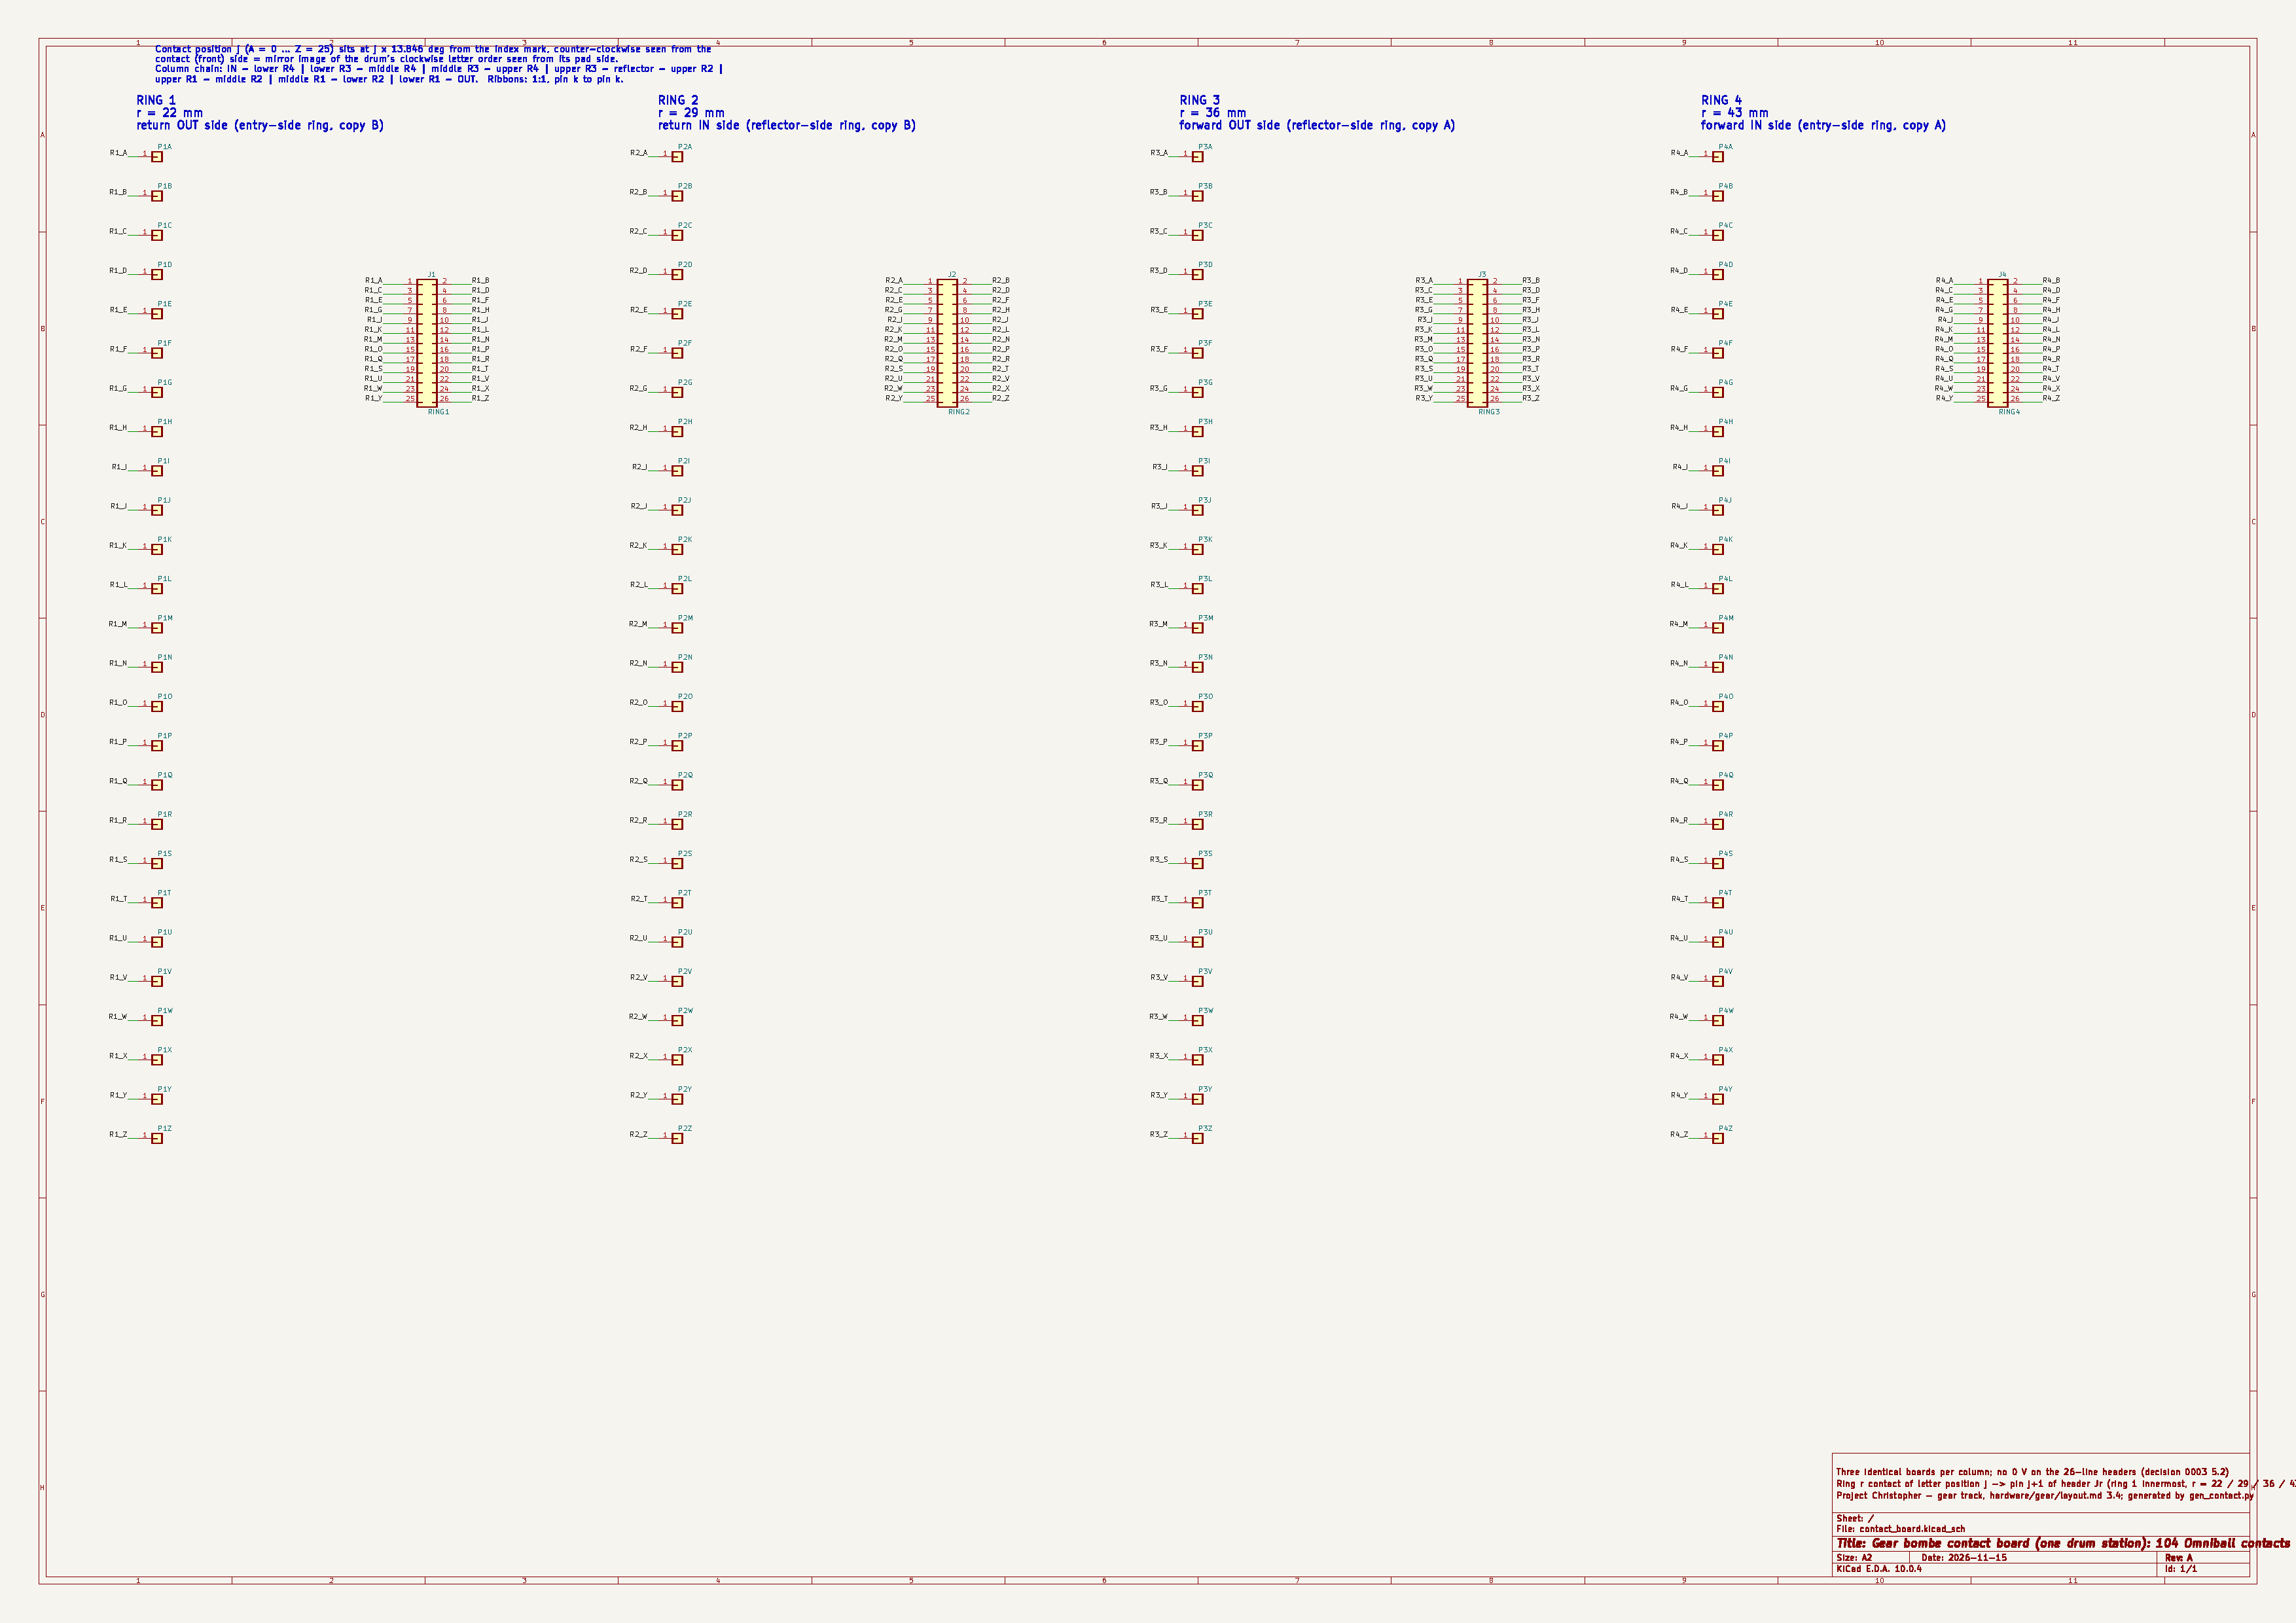
\includepdf[pages=-,pagecommand={\thispagestyle{plain}}]{figures/generated/sch_contact-board.pdf}}{}
\IfFileExists{figures/generated/sch_column-terminal.pdf}{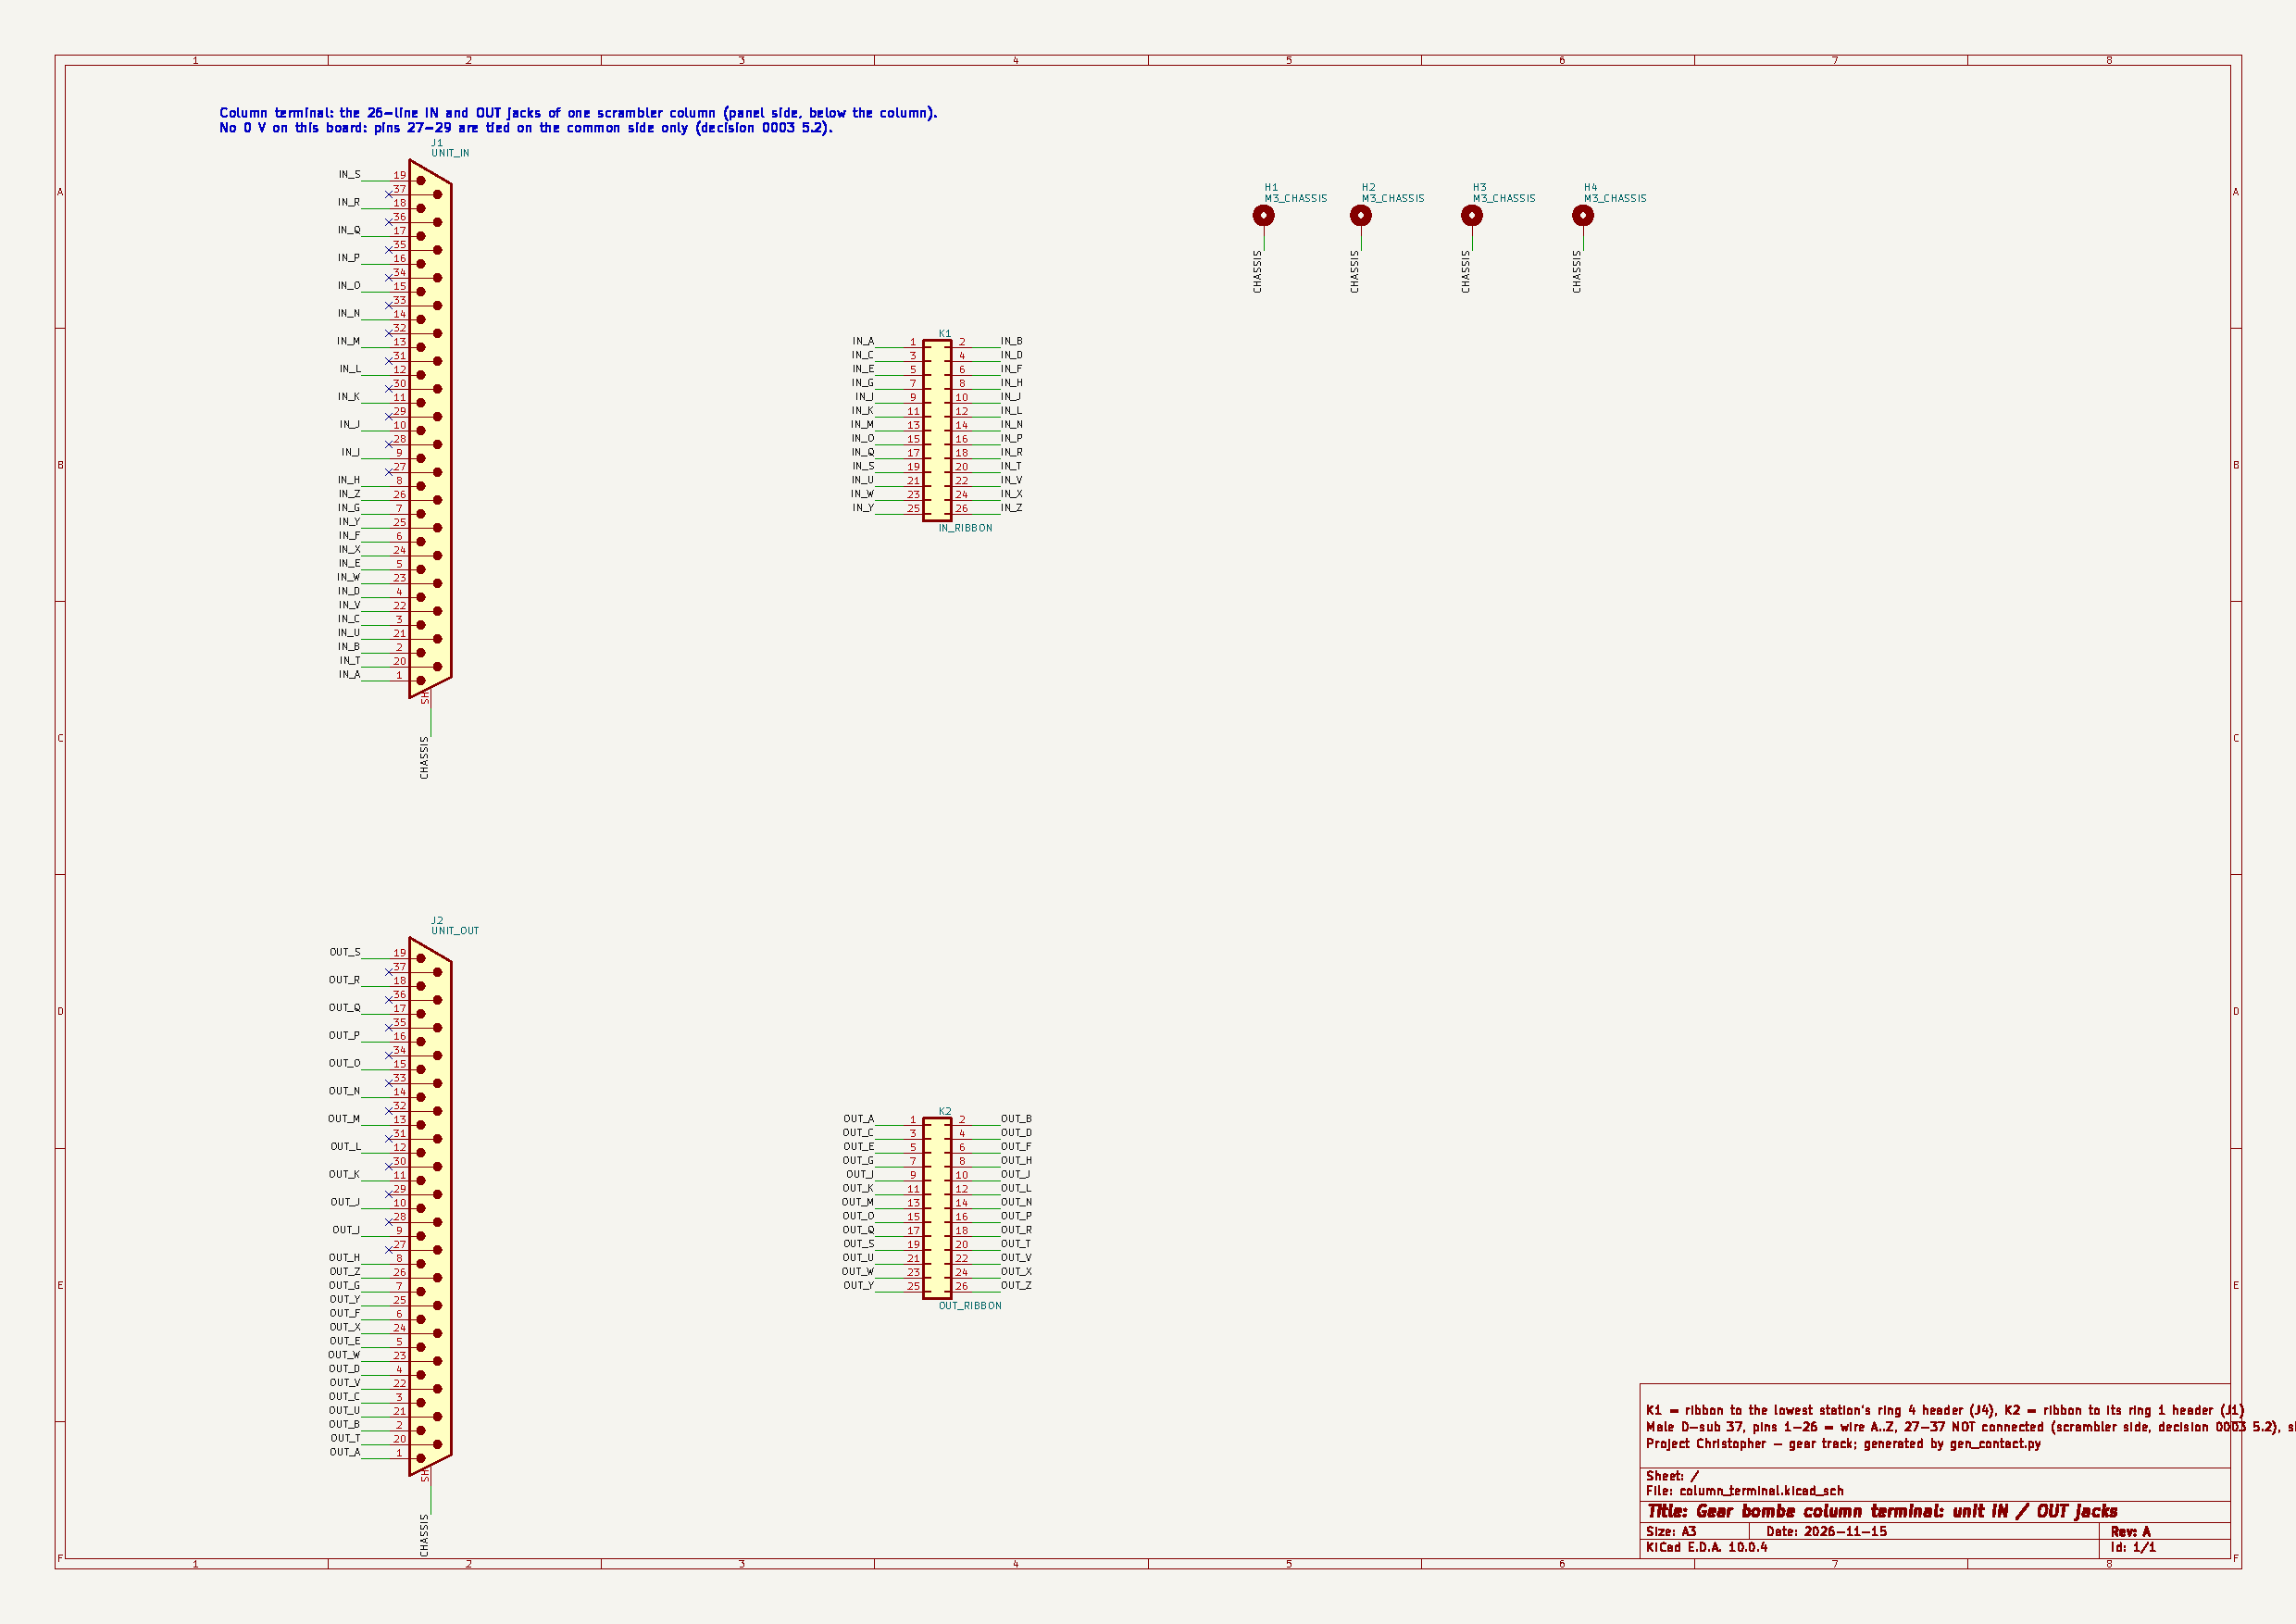
\includepdf[pages=-,pagecommand={\thispagestyle{plain}}]{figures/generated/sch_column-terminal.pdf}}{}
\IfFileExists{figures/generated/sch_reflector-card-b.pdf}{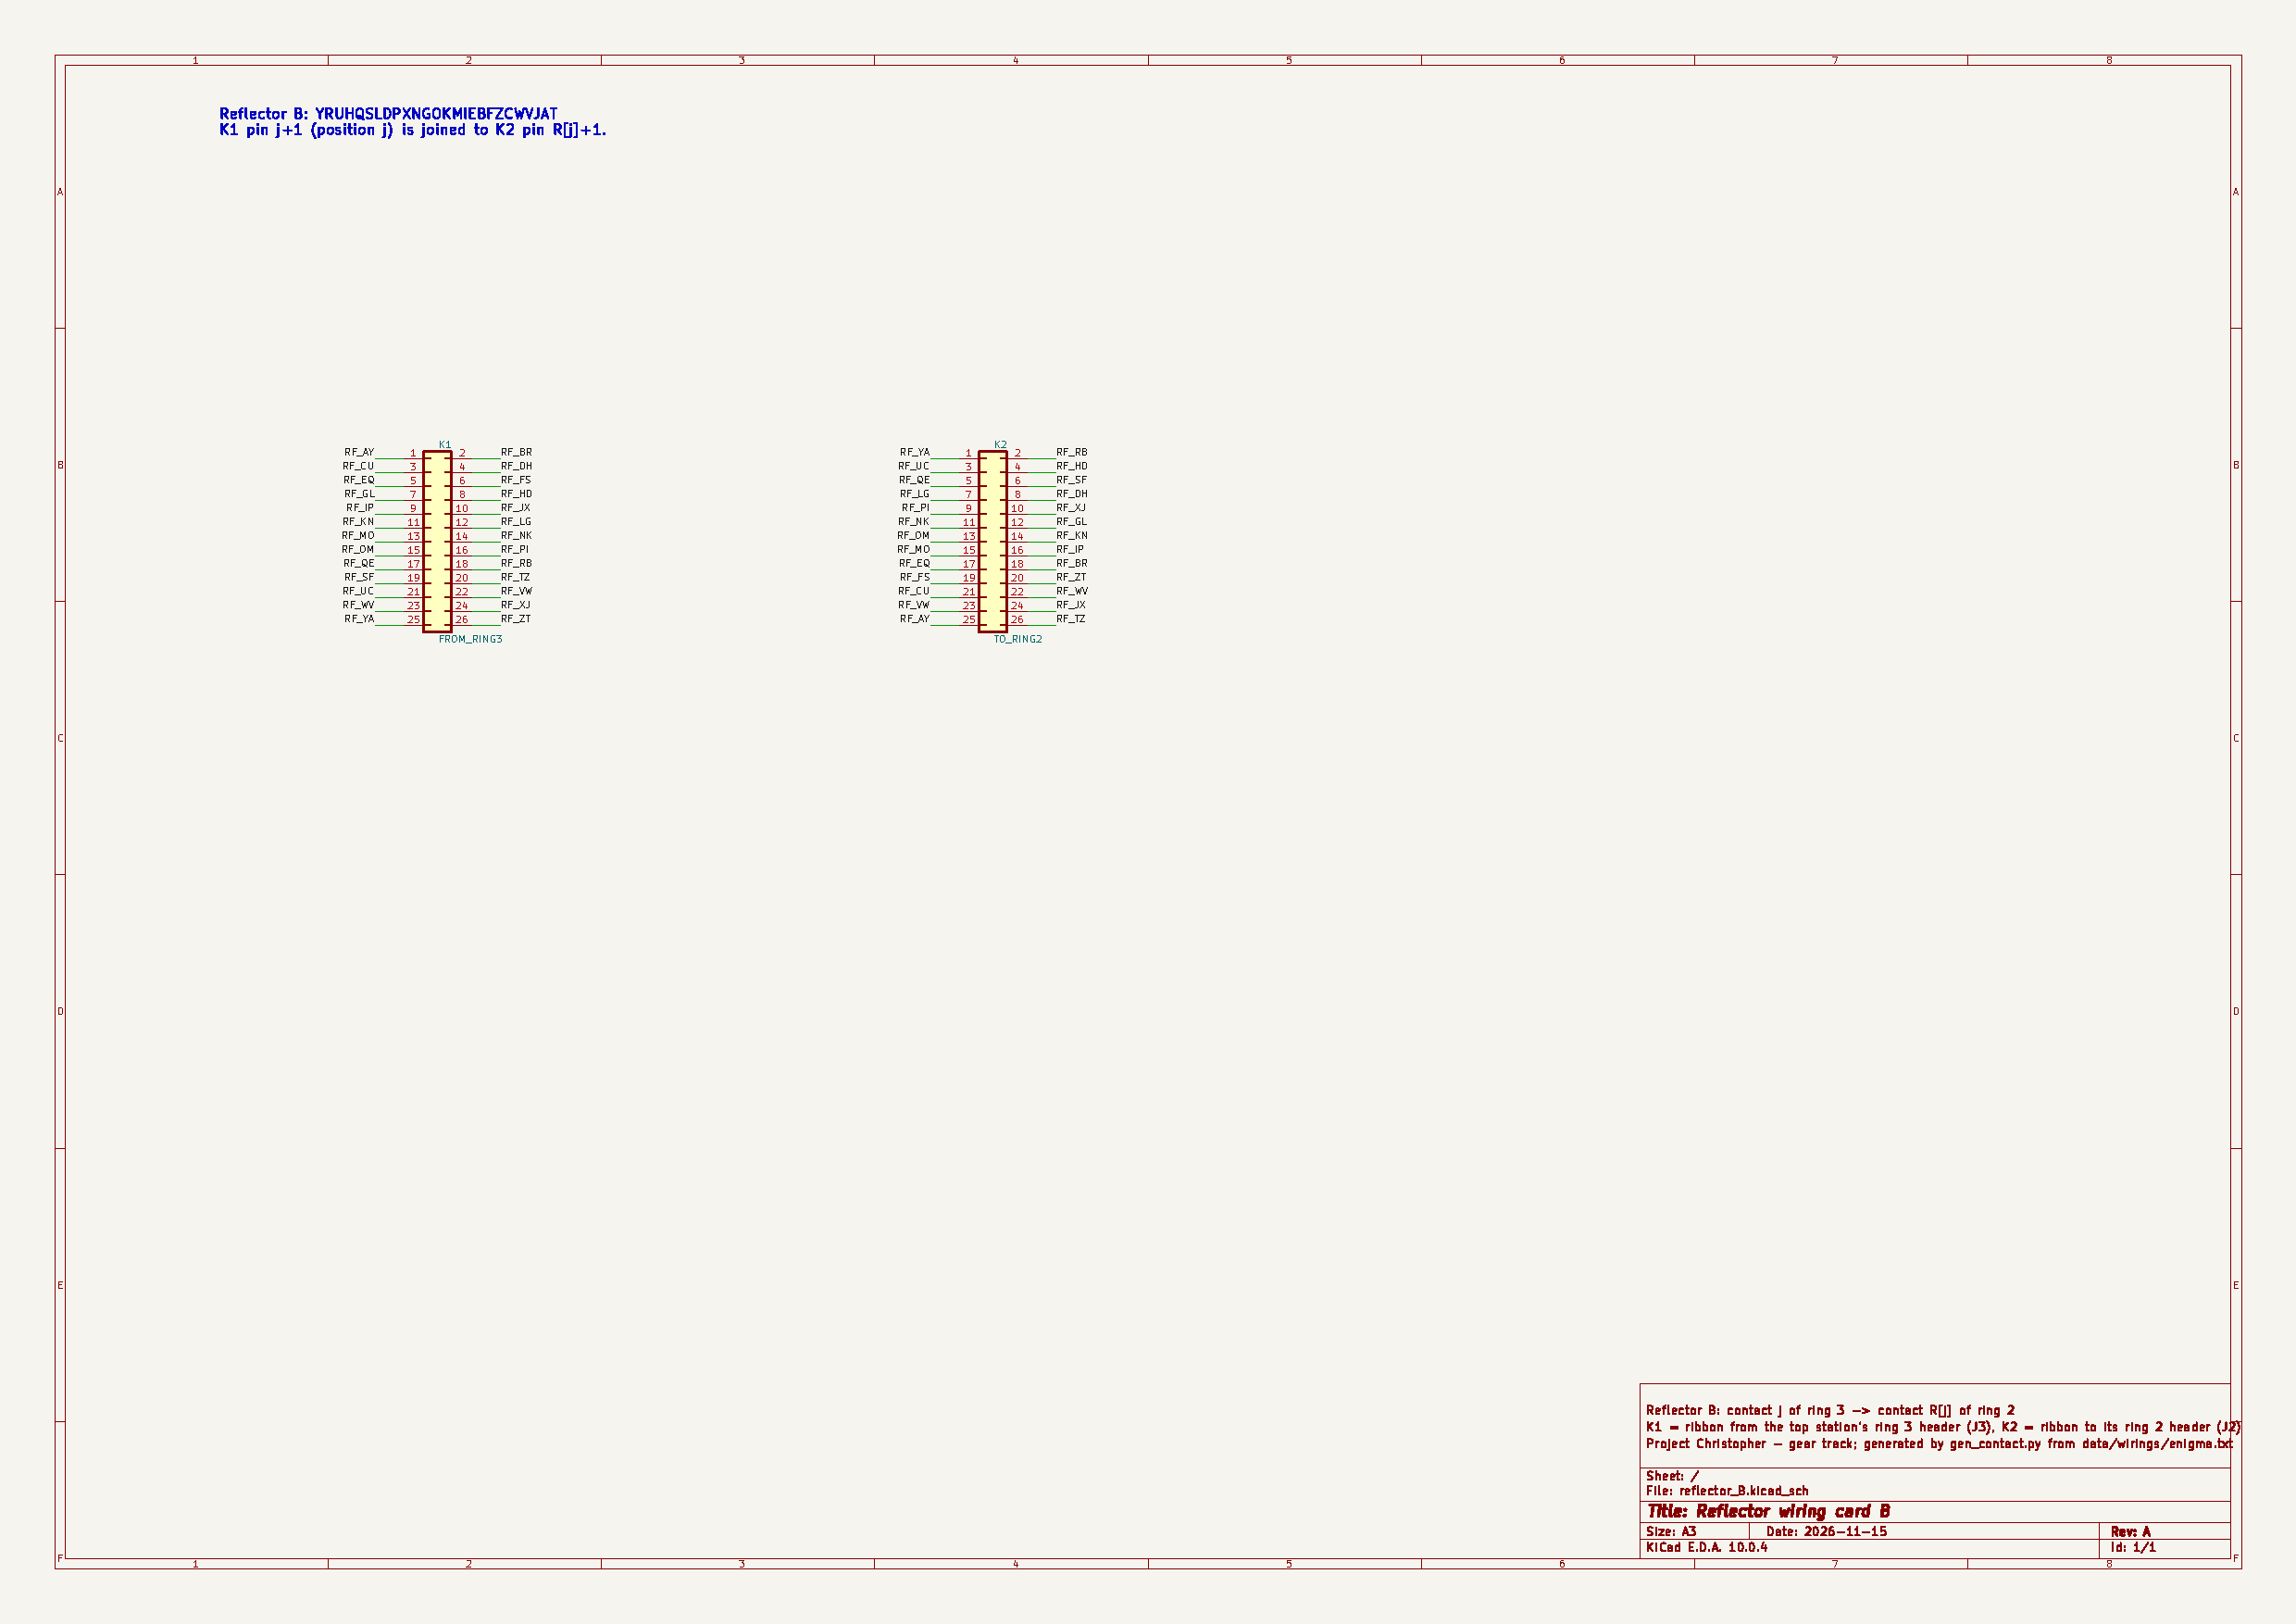
\includepdf[pages=-,pagecommand={\thispagestyle{plain}}]{figures/generated/sch_reflector-card-b.pdf}}{}

\section{대각선 보드(다섯 장)}\label{sch:diagonal}
글자 6/6/6/4/4개씩 나눈 다섯 장(D1--D5). 글자마다 수 D-sub 37 잭 두 개, 보드 사이는 64핀 IDC 세 가닥이다.
\code{hardware/common/diagonal-board/verify\_diagonal.py}가 다섯 넷리스트를 접속 리본으로 합쳐, 대각선 연결
325개(선 $w$의 글자 $c$ ↔ 선 $c$의 글자 $w$)가 정확히 그것만 이어지고 27--29번 0\,V가 한 넷임을 확인했다.
\IfFileExists{figures/generated/sch_diagonal-d1.pdf}{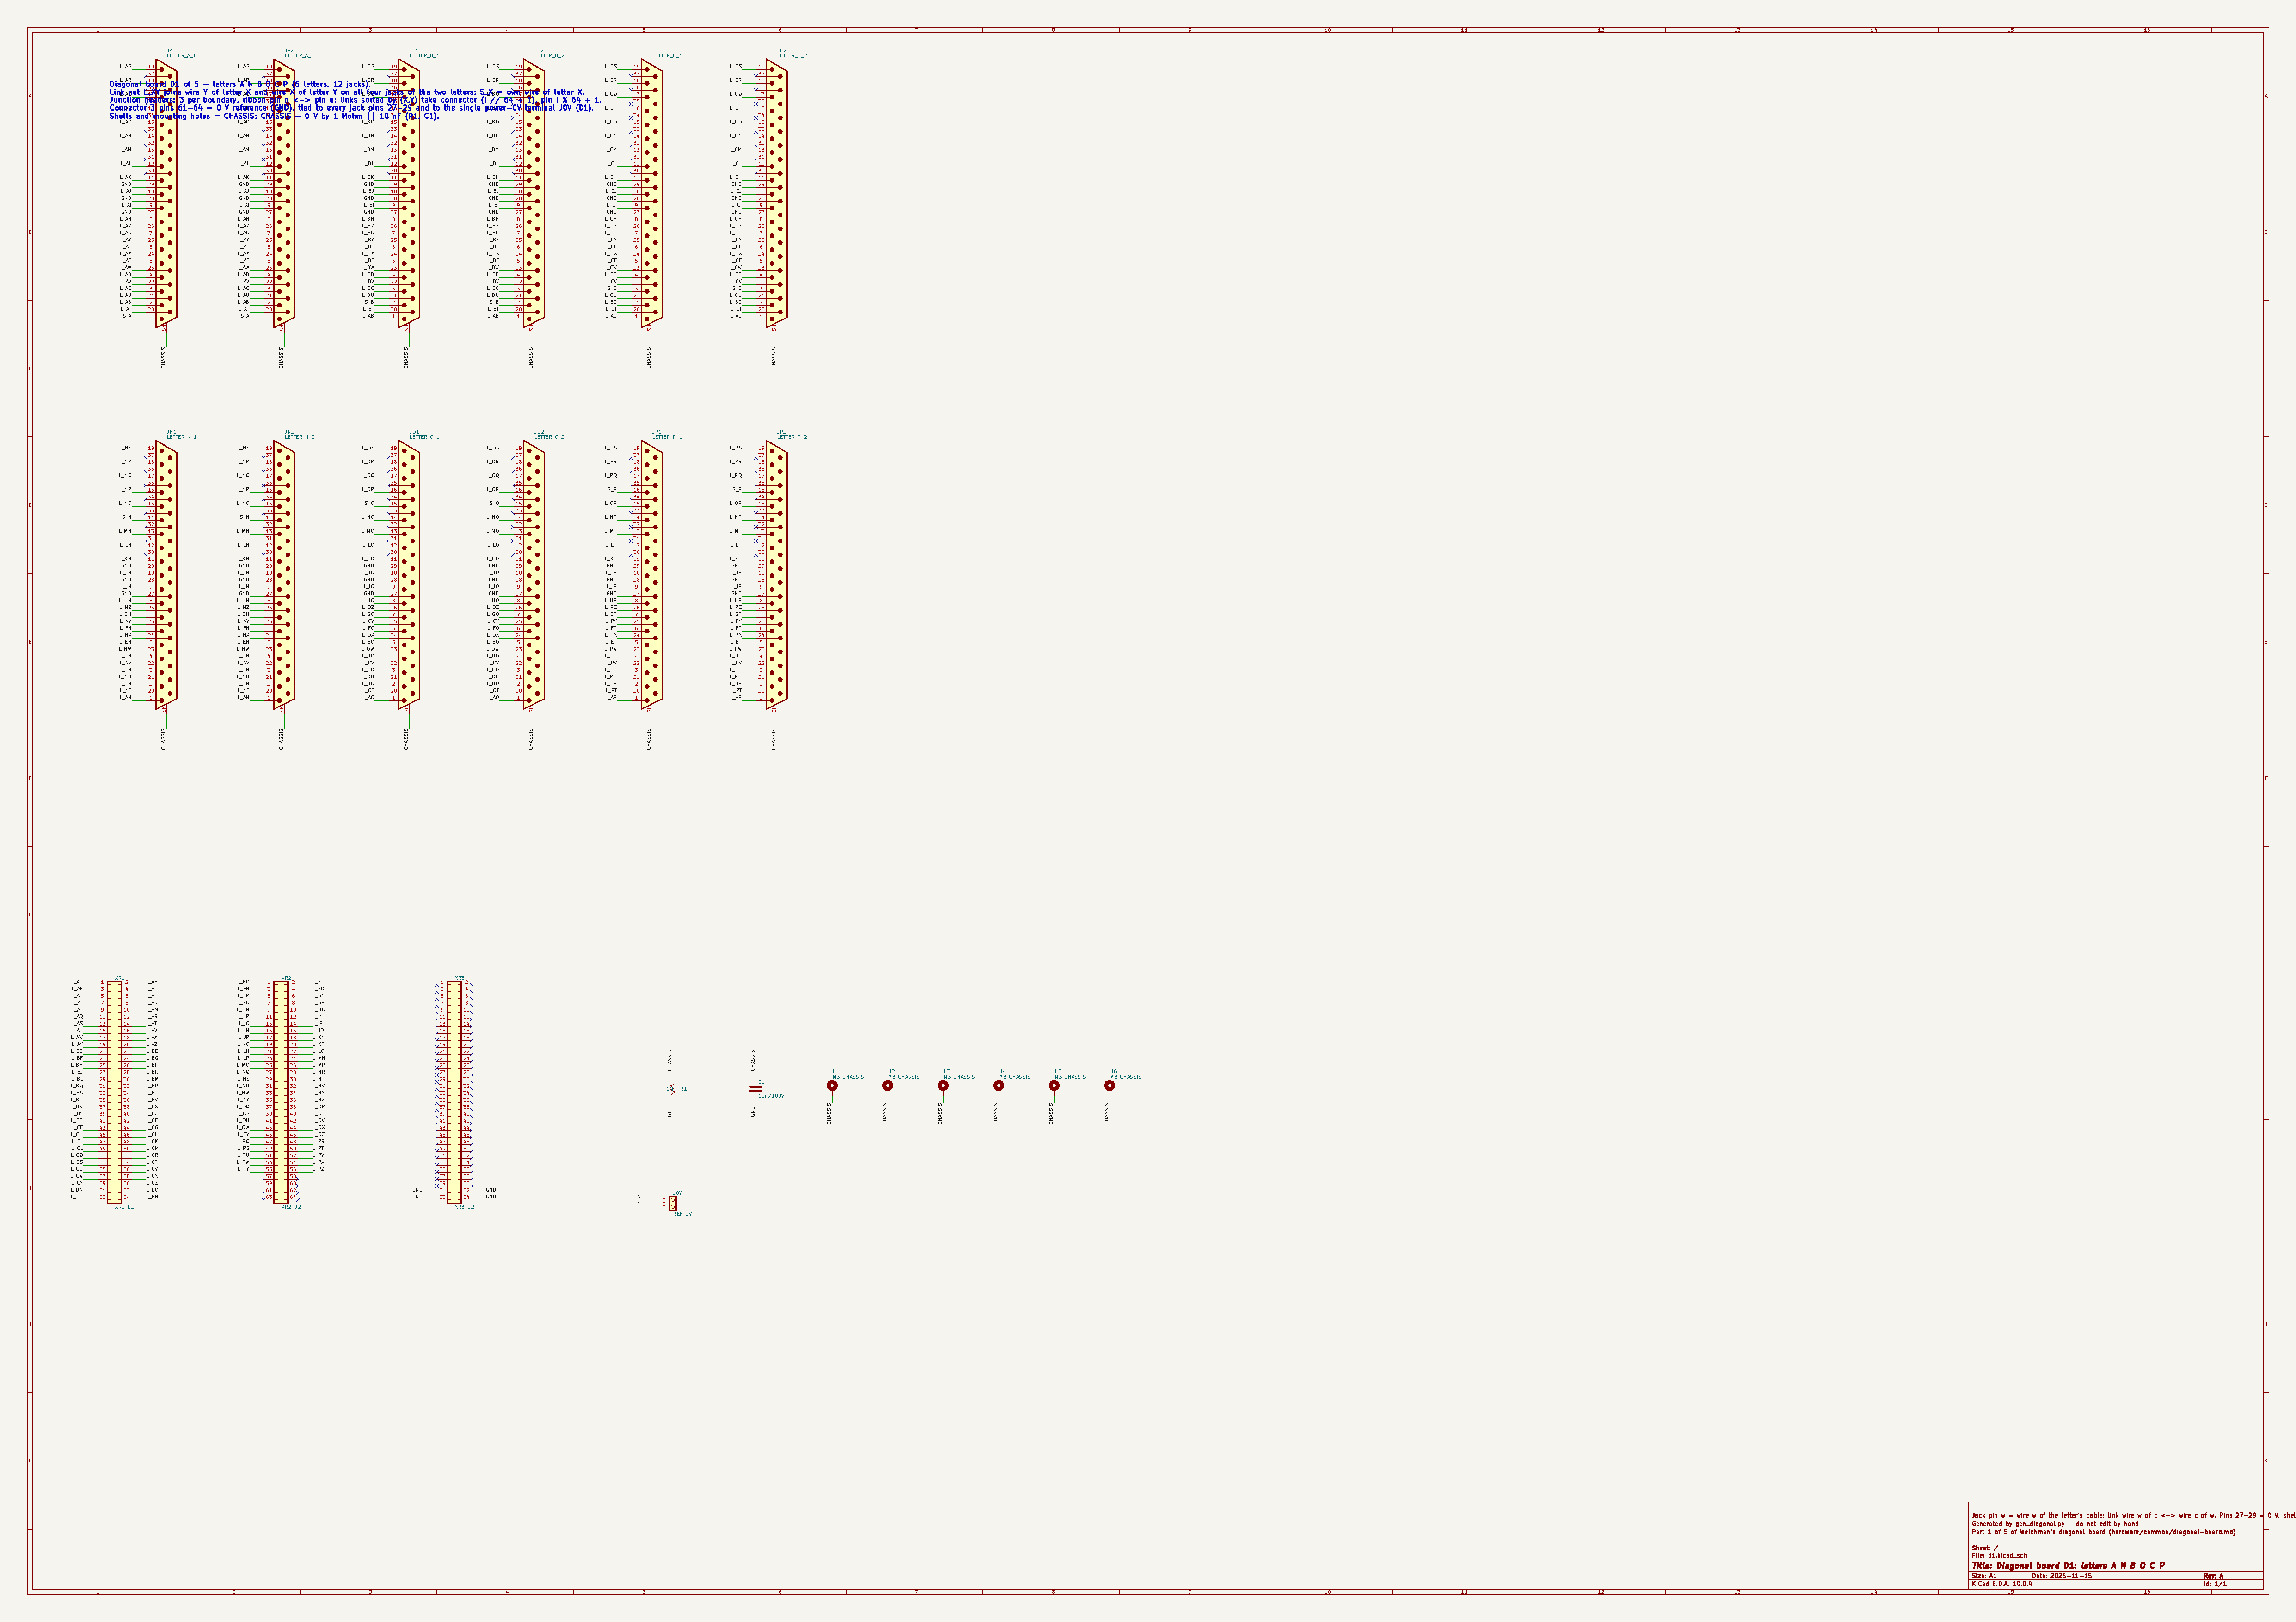
\includepdf[pages=-,pagecommand={\thispagestyle{plain}}]{figures/generated/sch_diagonal-d1.pdf}}{}
\IfFileExists{figures/generated/sch_diagonal-d2.pdf}{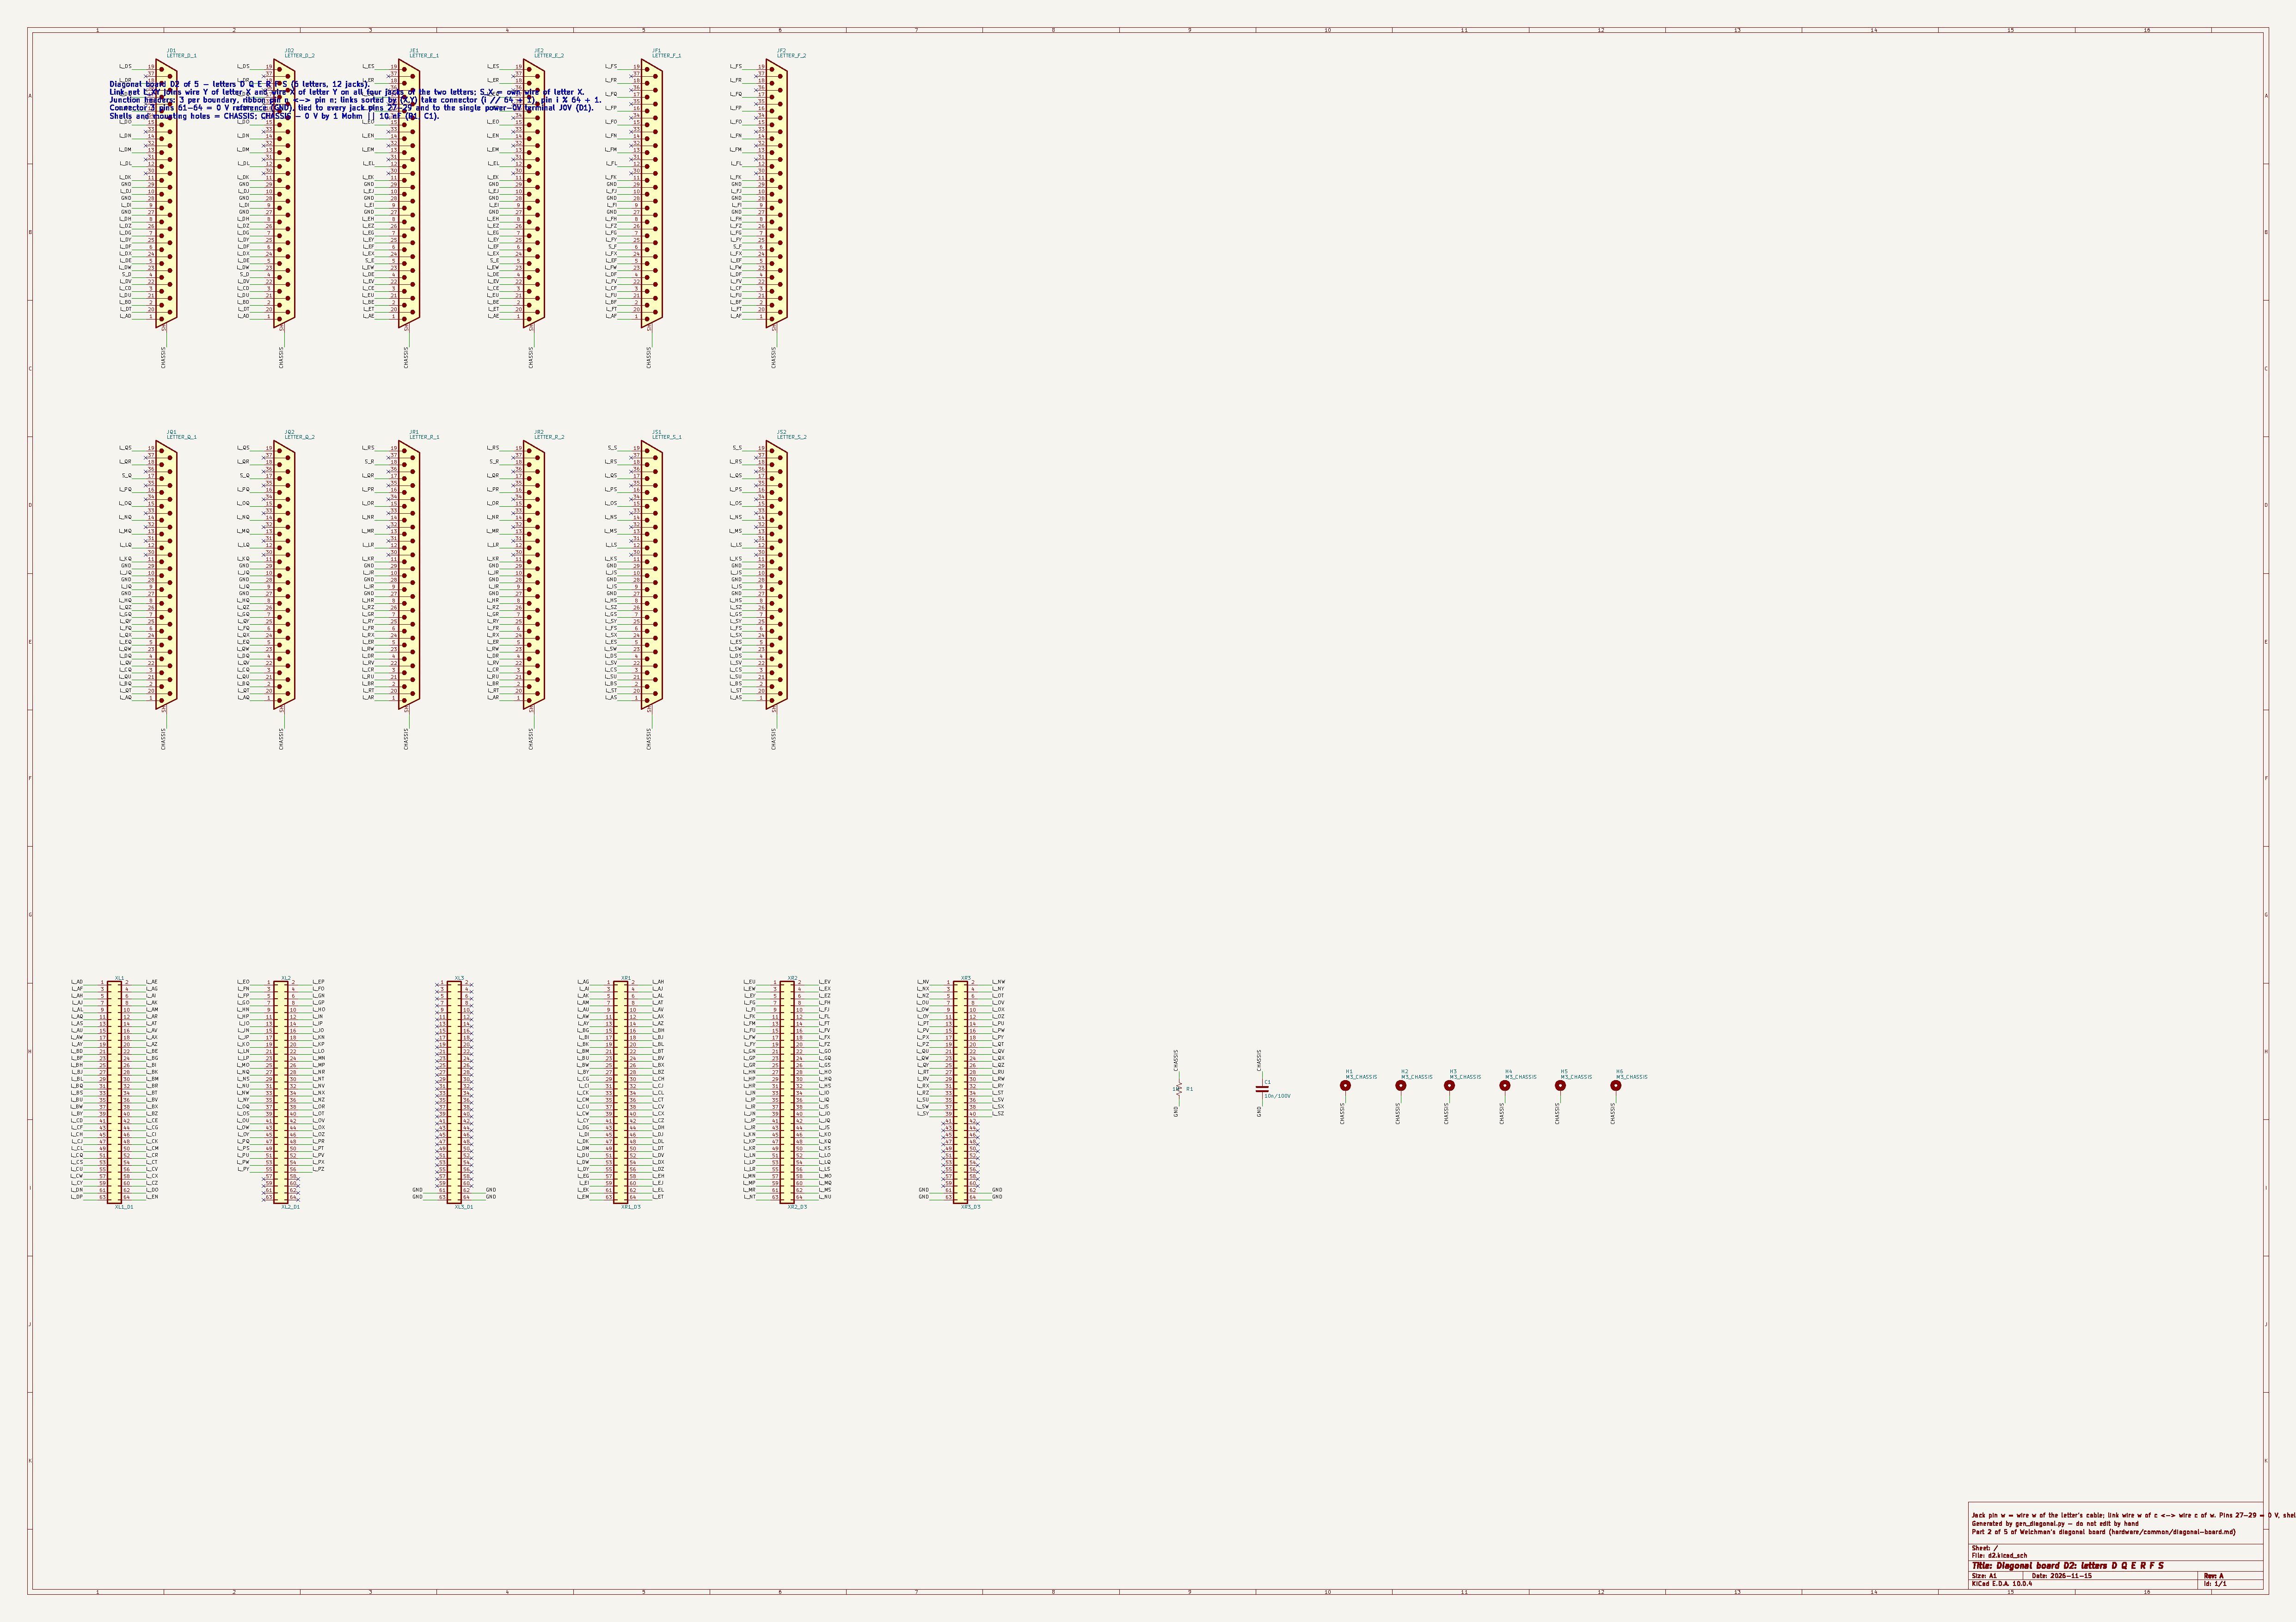
\includepdf[pages=-,pagecommand={\thispagestyle{plain}}]{figures/generated/sch_diagonal-d2.pdf}}{}
\IfFileExists{figures/generated/sch_diagonal-d3.pdf}{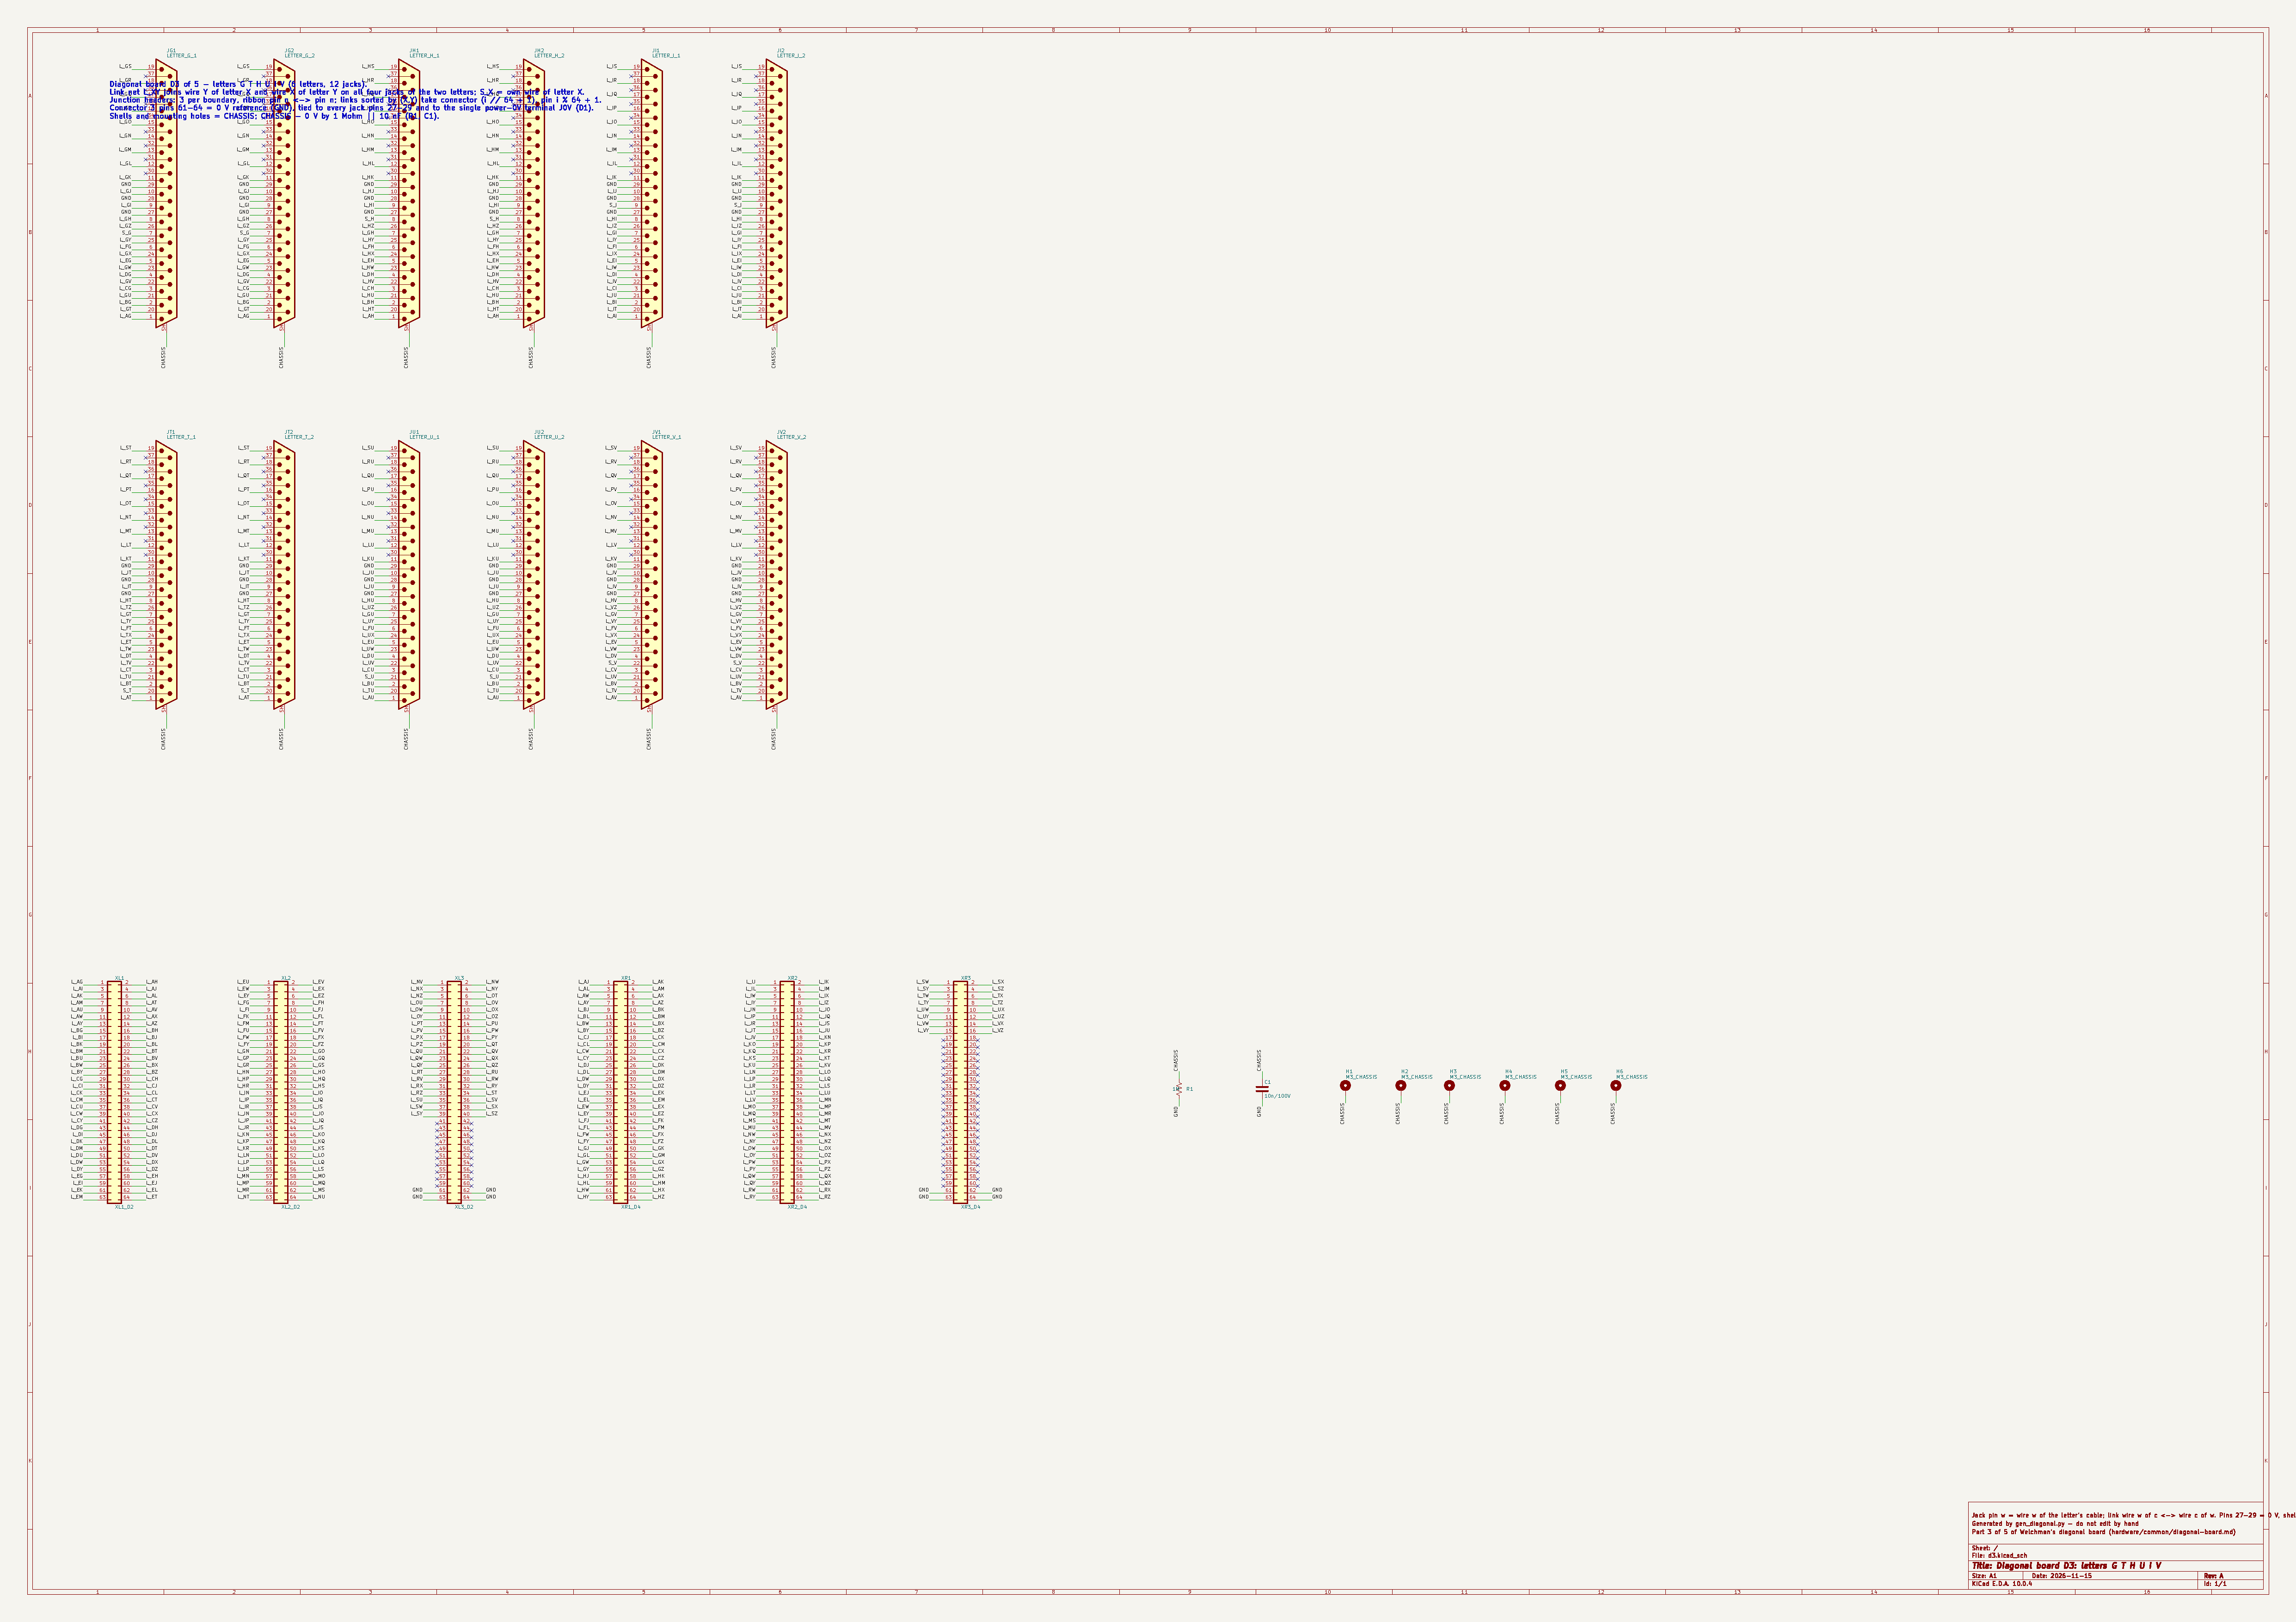
\includepdf[pages=-,pagecommand={\thispagestyle{plain}}]{figures/generated/sch_diagonal-d3.pdf}}{}
\IfFileExists{figures/generated/sch_diagonal-d4.pdf}{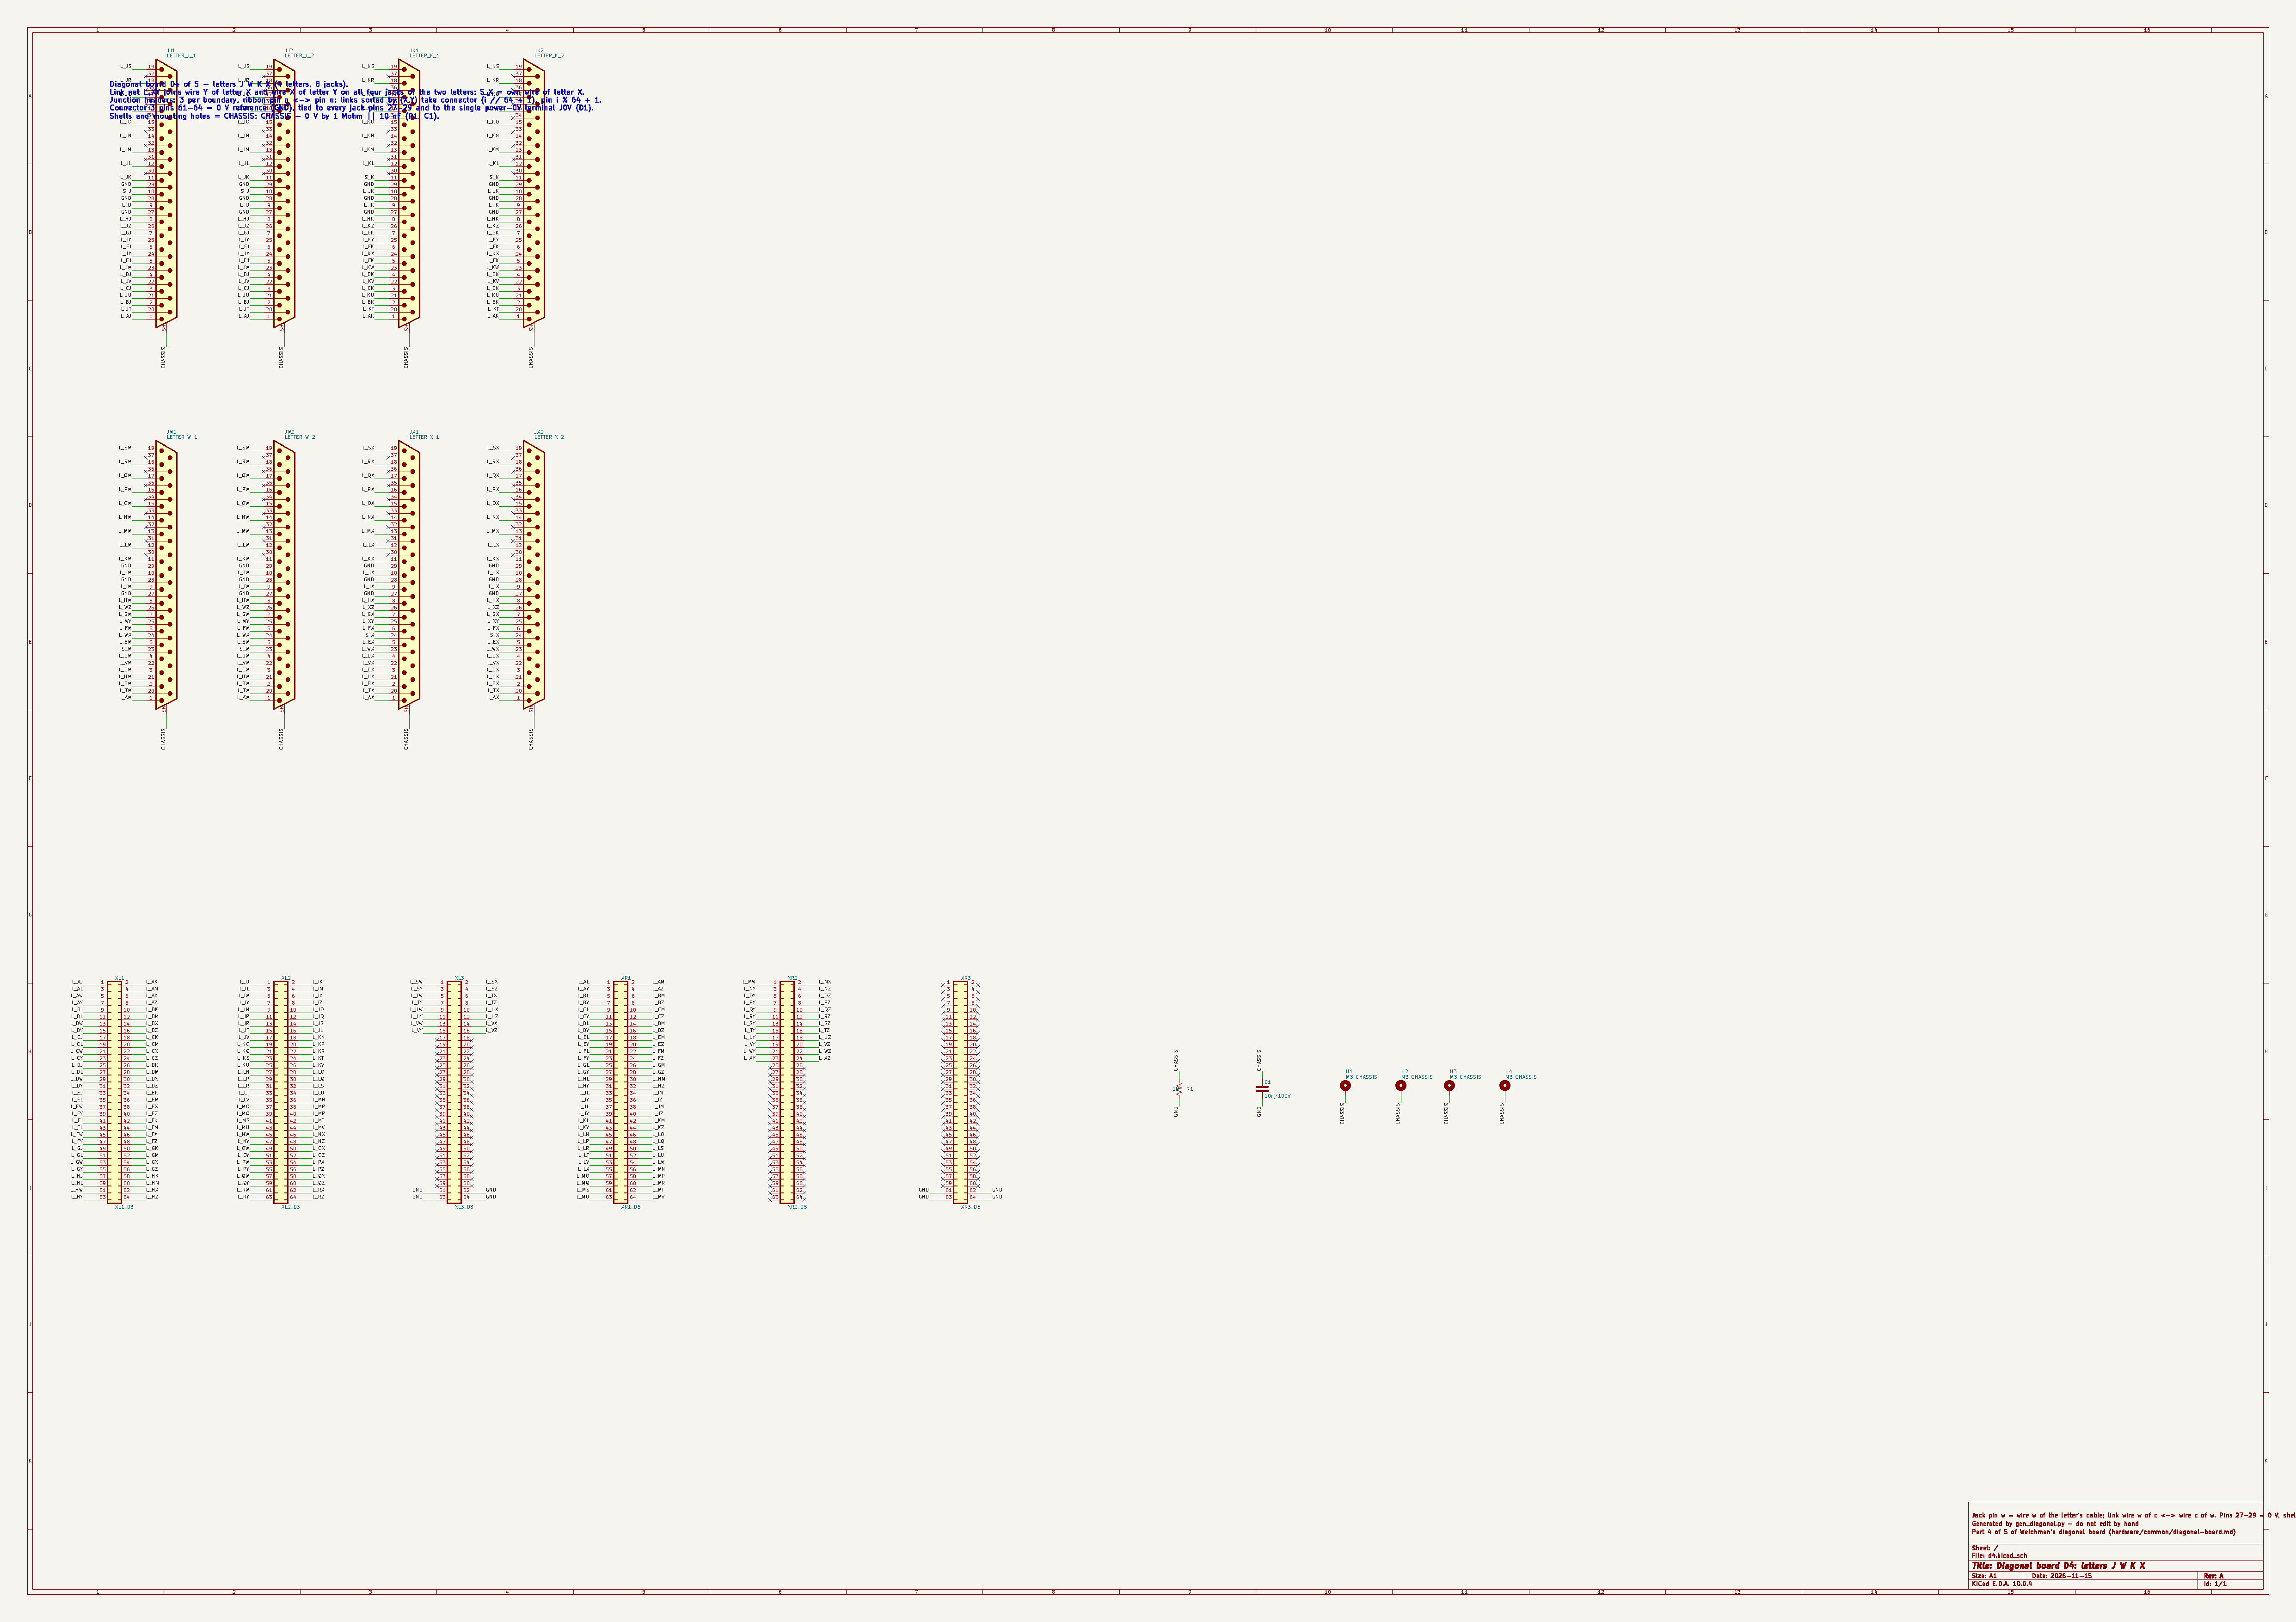
\includepdf[pages=-,pagecommand={\thispagestyle{plain}}]{figures/generated/sch_diagonal-d4.pdf}}{}
\IfFileExists{figures/generated/sch_diagonal-d5.pdf}{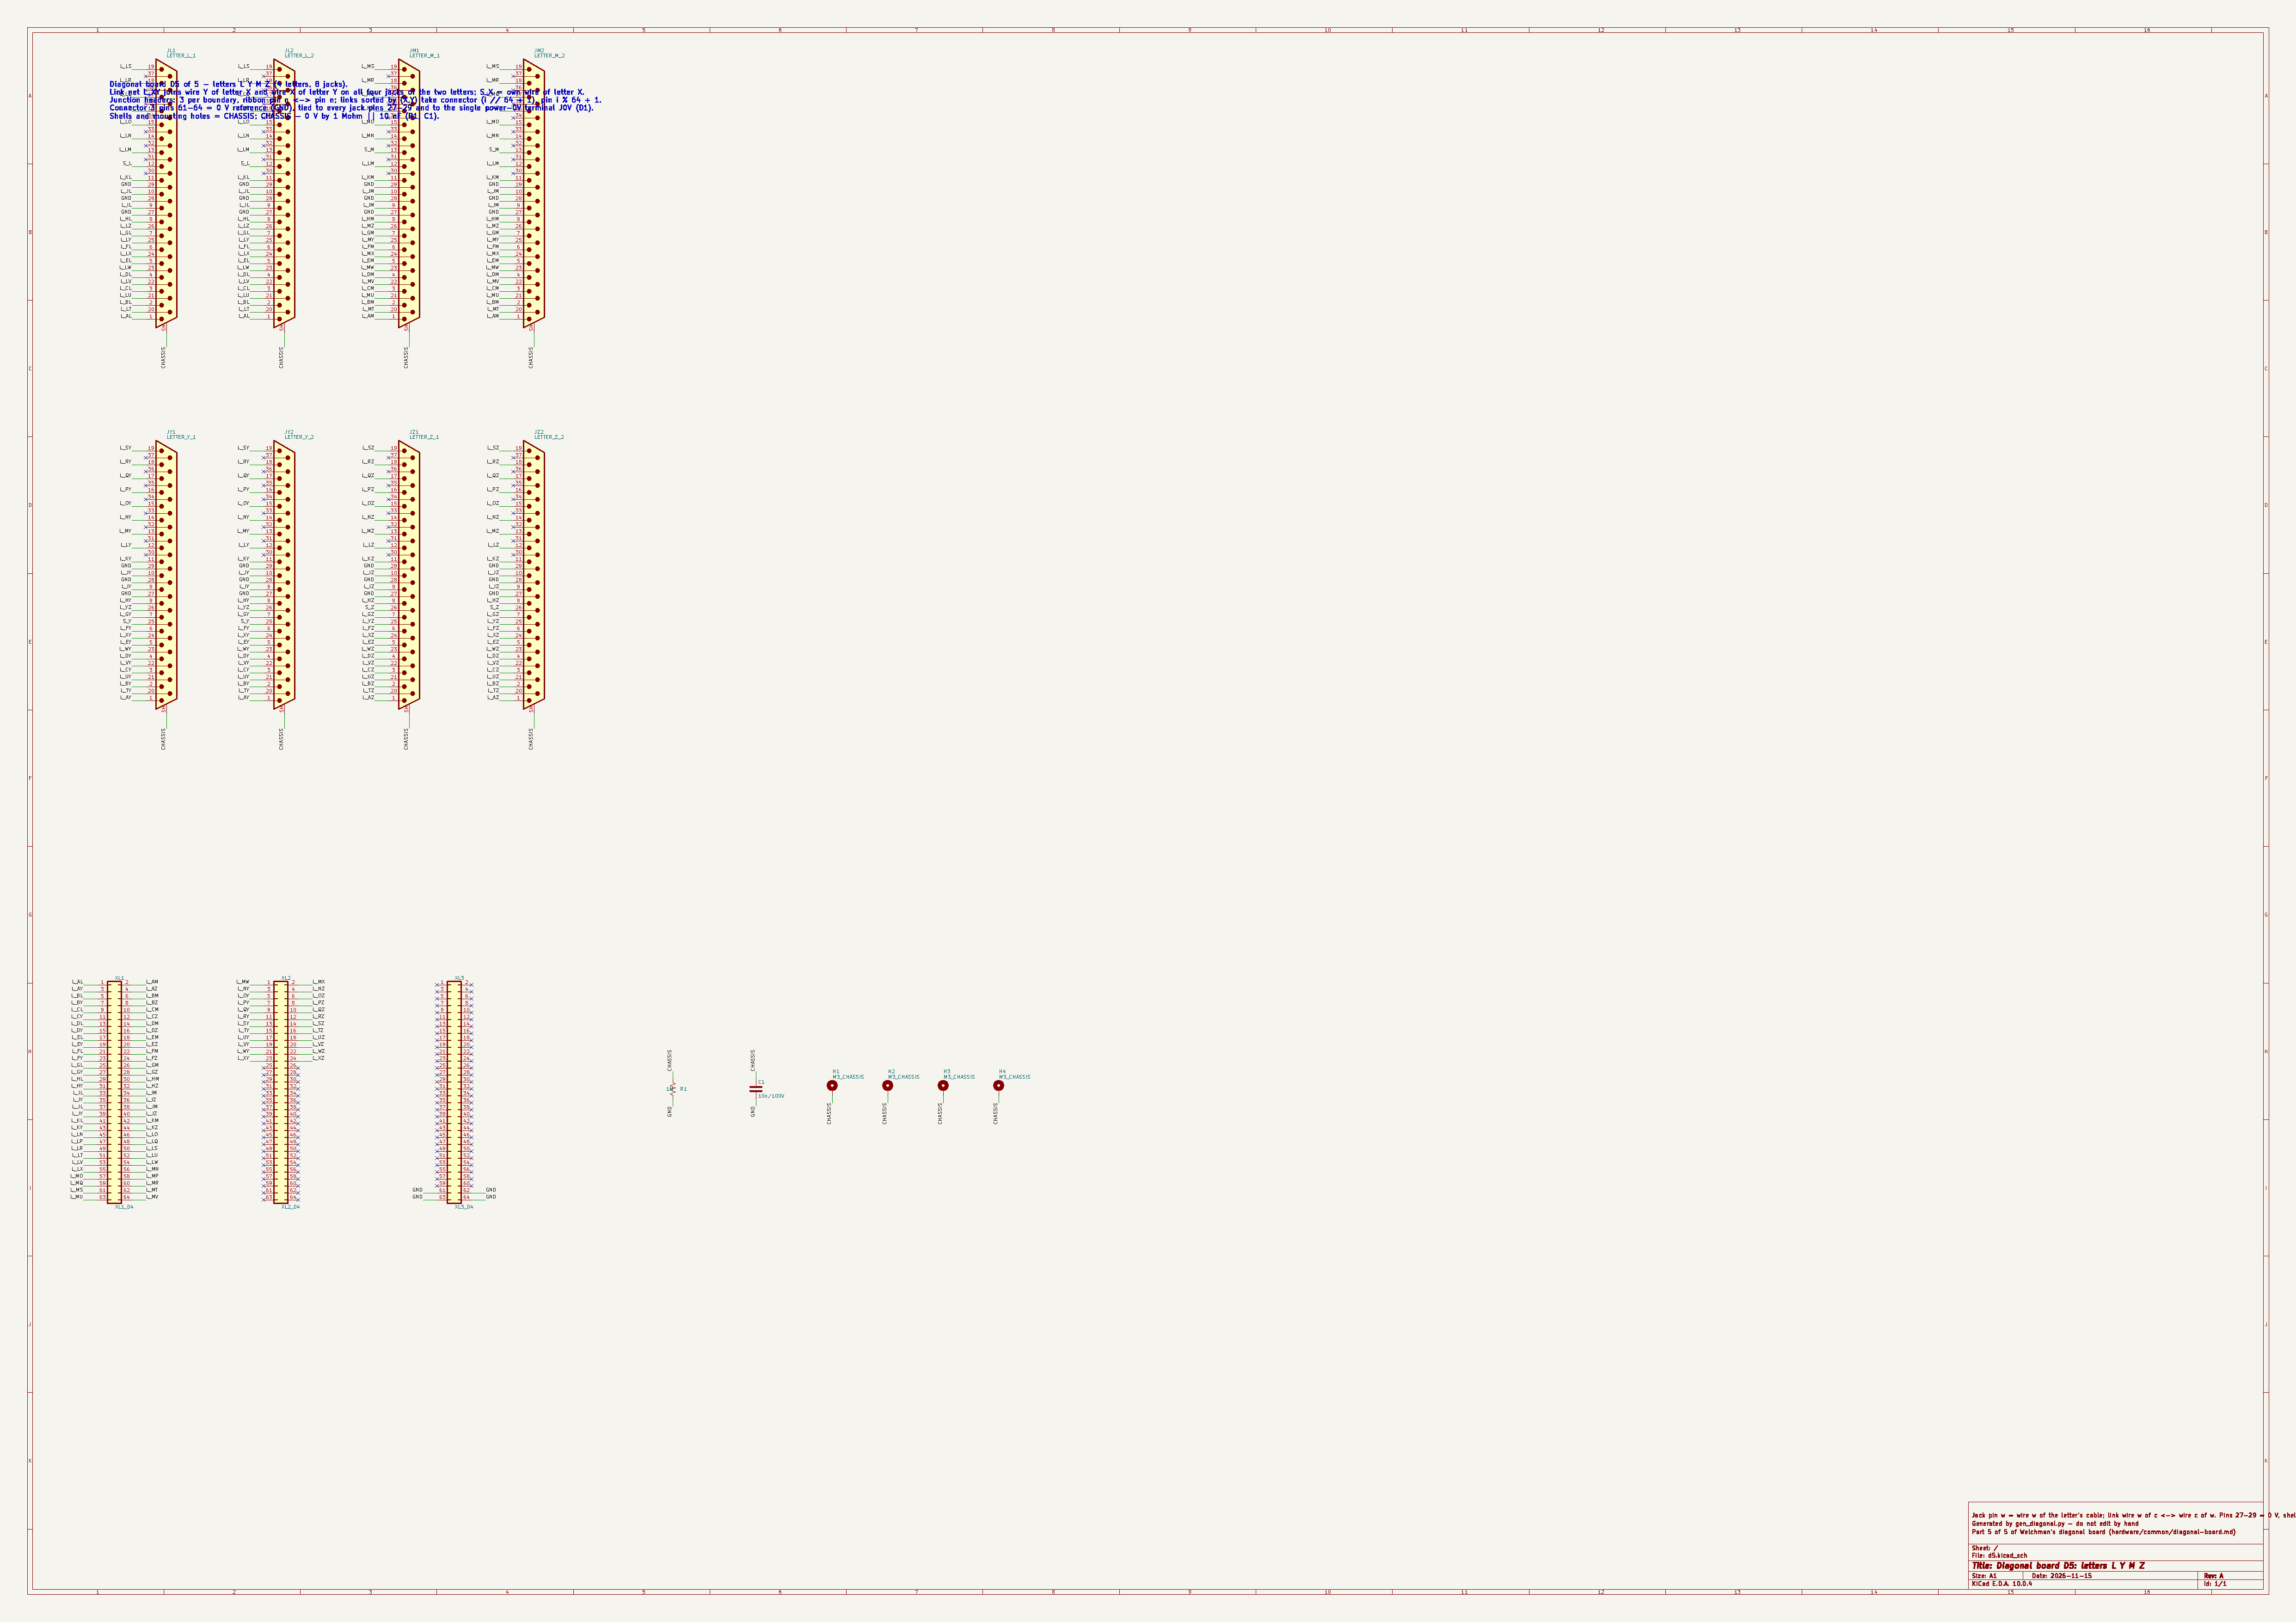
\includepdf[pages=-,pagecommand={\thispagestyle{plain}}]{figures/generated/sch_diagonal-d5.pdf}}{}

\section{메뉴 패치 패널}\label{sch:patch-panel}
공통 잭 4묶음 × 4개, 테스트 레지스터 잭, 탐색 잭과 시험 전압 플러그를 꽂는 26구멍, 0\,V(27--29번)를 묶는 곳이다.
글자 잭은 대각선 보드에 있다. \code{verify\_patch.py}는 플러그를 각 구멍에 꽂은 경우까지 시뮬레이션해 확인했다.
\IfFileExists{figures/generated/sch_patch-panel.pdf}{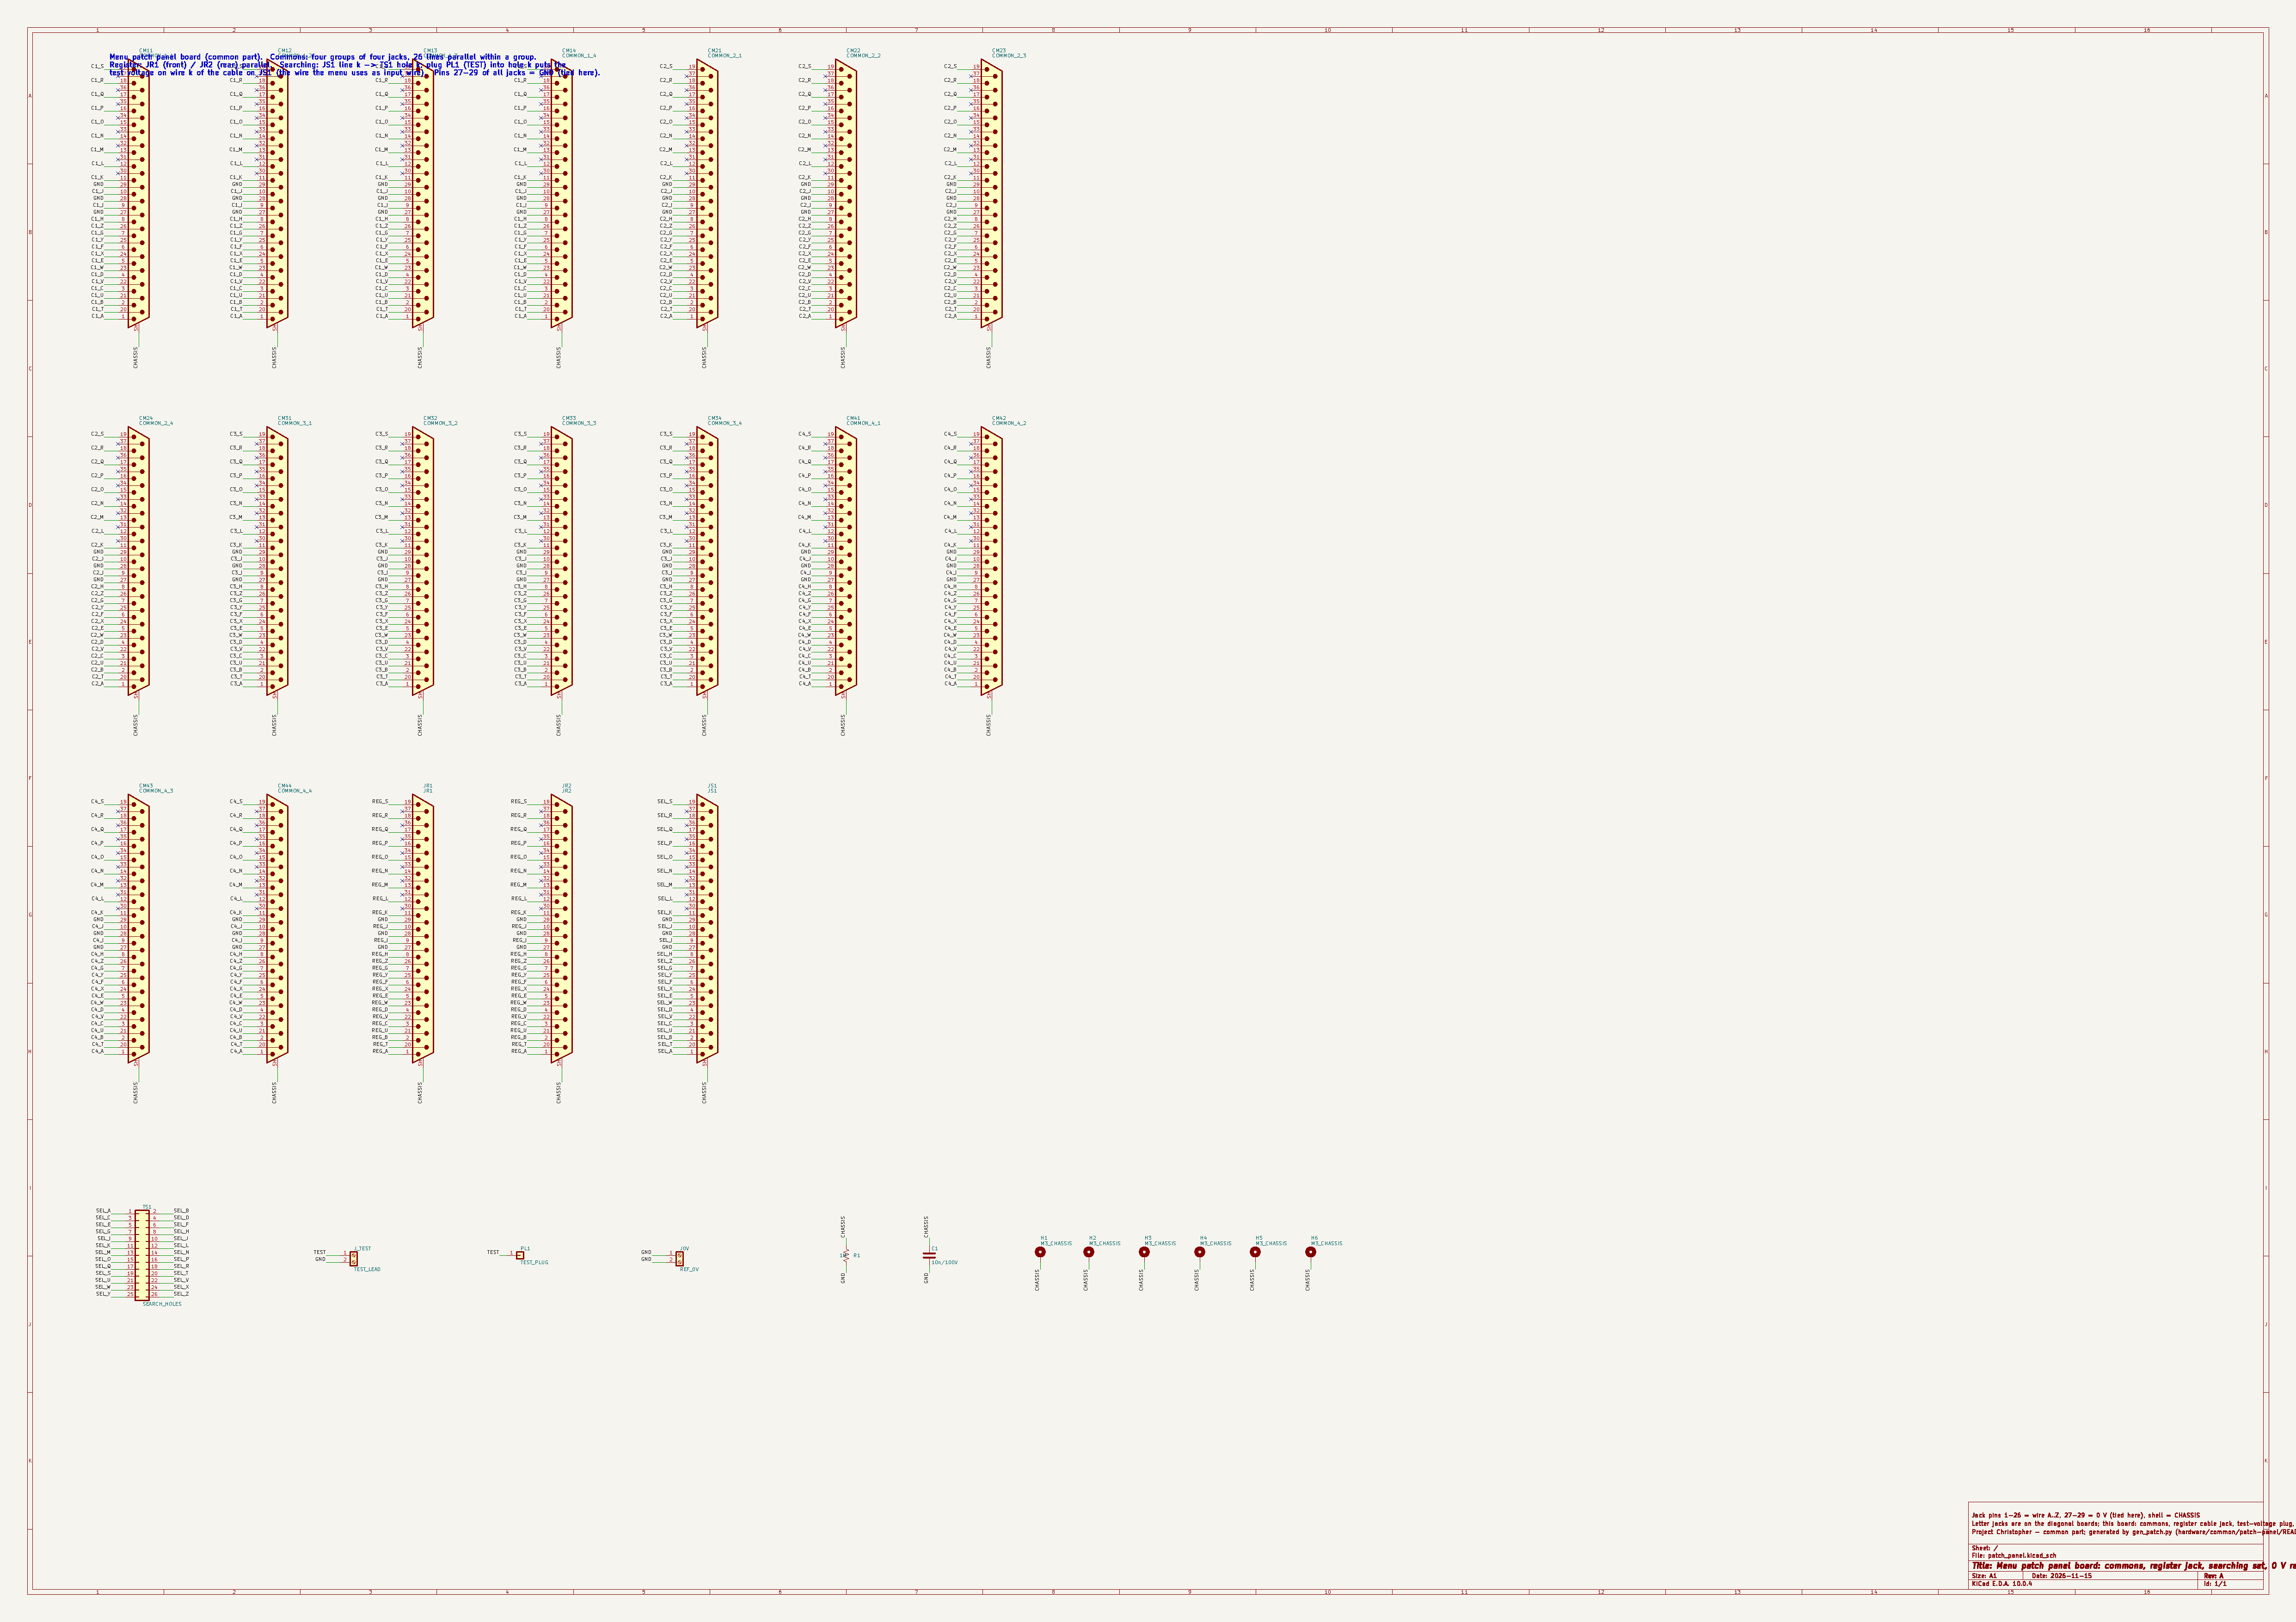
\includepdf[pages=-,pagecommand={\thispagestyle{plain}}]{figures/generated/sch_patch-panel.pdf}}{}

% PCB 배치 부록 (그림은 report/figures/make_pcb_figures.py로 생성).
\chapter{PCB 배치}\label{app:pcb}

회로도 부록(\ref{app:schematics})의 다섯 보드를 기판에 배치한 결과다. 그림은 앞면의 배치도로, 외곽, 부품의 외형,
실크, 부품이 차지하는 경계를 그렸다. \emph{배선은 아직 하지 않았다.} 보드 파일에는 외곽, 장착 구멍, 모든 부품의
자리와 방향, 회로도에서 가져온 넷(어느 패드끼리 이어야 하는가), 설계 규칙이 들어 있고 동선은 하나도 없다.

\section{배치를 정한 원칙}

\paragraph{왜 배치까지만 했는가.} 이 보드들의 배선은 같은 모양의 되풀이다. 시프터는 릴레이 130개가, 테스트
레지스터는 레인 26개가, 계수기는 자리 다섯이 같은 회로다. 되풀이되는 단위 하나의 배선을 사람이 정하고 나머지에
옮기는 것이 자동 배선보다 읽기 쉽고 고치기 쉬운 기판을 만든다. 배치는 그 전제다. 되풀이 단위가 기판 위에서도
같은 모양으로 놓여 있어야 한 단위의 배선을 옮길 수 있다. 그래서 배치도 회로도처럼 스크립트가 만든다
(\code{gen\_*\_pcb.py}). 부품의 자리는 ``몇째 단의 몇째 선''에서 계산되는 좌표이고, 같은 입력은 바이트 단위로 같은
파일을 낸다.

\paragraph{공통 규칙.}
\begin{itemize}
\item \textbf{신호가 흐르는 방향으로 놓는다.} 입력 커넥터에서 출력 커넥터까지 선이 되돌아가지 않게 한다. 26선이
나란히 가는 보드에서는 되돌아가는 선 하나가 26번의 교차가 된다.
\item \textbf{커넥터는 가장자리에, 같은 종류는 같은 변에.} 케이블이 보드 위를 가로지르지 않는다. 릴레이식의 세
보드는 입력이 왼쪽, 출력이 오른쪽이어서 카드 케이지에 나란히 꽂았을 때 케이블이 한 방향으로 흐른다.
\item \textbf{코일의 다이오드는 코일 옆에.} 코일이 꺼질 때의 전류가 도는 고리를 작게 한다.
\item \textbf{릴레이식의 세 보드는 같은 카드 크기}(250 × 228~mm, 구멍은 모서리에서 5~mm, M3 넷)다. 시프터 보드가
이 크기를 정했고 계수기 두 장이 따랐다. 케이지의 슬롯이 한 종류가 된다.
\end{itemize}

\paragraph{확인하는 것.} 배치만 한 기판에서도 틀릴 수 있는 것이 있다. 부품이 빠지거나, 풋프린트가 회로도와
다르거나, 패드에 붙은 넷이 회로도와 다르거나, 부품끼리 겹치는 것이다. 보드마다 검증 스크립트가 다음을 본다.
(1) 회로도의 부품이 모두 기판에 있고 풋프린트가 같다. (2) 패드마다의 넷이 회로도의 넷리스트와 정확히 같다.
(3) KiCad의 설계 규칙 검사(DRC)에서 위반이 0건이고, 남는 것은 ``아직 이어지지 않은 연결''뿐이다. (4) 패드 둘의
넷을 바꾼 기판을 넣으면 검사가 실패한다. (5) 두 번 생성한 파일이 같다.

\begin{table}[ht]
\centering
\caption{배치한 보드. 남은 연결은 배선해야 할 패드 쌍의 수다.}
\label{tab:pcb-boards}
\small
\begin{tabularx}{\linewidth}{>{\raggedright\arraybackslash}Xlrrr}
\toprule
보드 & 크기, 층 & 부품 & 넷 & 남은 연결 \\
\midrule
릴레이 시프터 & 250 × 228 mm, 4층 & 275 & --- & 1,120 \\
릴레이 계수기(공통) & 250 × 228 mm, 4층 & 261 & 211 & 539 \\
릴레이 계수기(유닛) & 250 × 228 mm, 4층 & 196 & 203 & 445 \\
테스트 레지스터 & 250 × 140 mm, 2층 & 258 & 288 & --- \\
단위 시험기 & 290 × 116 mm, 4층 & 446 & 445 & --- \\
\bottomrule
\end{tabularx}
\end{table}

(부품 수는 장착 구멍을 뺀 것이다. 단위 시험기만 구멍 여섯을 포함한다. 빈칸은 세지 않은 값이다. DRC의 보고서는
연결 안 된 항목을 499건까지만 적으므로, 남은 연결은 기판의 연결 정보에서 따로 센다.)

\newcommand{\pcbfigure}[3]{%
  \IfFileExists{figures/generated/pcb_#1.pdf}{%
    \begin{figure}[p]
      \centering
      \includegraphics[width=\linewidth,height=0.8\textheight,keepaspectratio]{figures/generated/pcb_#1.pdf}
      \caption{#2}\label{fig:pcb-#1}
    \end{figure}}{}%
  #3}

% ======================================================================
\section{릴레이 시프터 보드}

\paragraph{배치.} 릴레이를 5열 × 26행의 격자로 놓았다(그림~\ref{fig:pcb-shifter-board}). 열이 단(왼쪽부터 1, 2, 4,
8, 16칸)이고 행이 선(위가 A)이다. 릴레이를 90° 돌려 한 줄의 핀(코일, 놓임 쪽, 공통, 동작 쪽)이 가는 길의 행이
되고 5.08~mm 위의 다른 줄이 오는 길의 행이 되게 했다. 그러면 신호가 왼쪽 커넥터에서 들어와 다섯 열을 차례로
지나 오른쪽 커넥터로 나간다. 입력 둘과 제어 커넥터가 왼쪽 변, 출력 둘이 오른쪽 변이다. 다이오드는 릴레이마다
코일 핀의 왼쪽에 세로로, 단의 표시등은 열의 아래에 있다.

\paragraph{크기.} 처음에는 160 × 200~mm를 생각했으나 들어가지 않는다. 릴레이 하나가 차지하는 경계가
7.9 × 15.3~mm여서 한 열 26개만으로 208~mm다. 높이 228~mm는 여기서 나온다. 폭은 배선이 정한다. 한 단은 26선을
$s$칸 아래로(오는 길은 위로) 옮겨 다음 열에 넘기는데, 이 옮김이 열 사이에서 세로로 달리는 선이 된다. 이동량이
클수록 겹치는 세로 선이 많아 16칸 단에서는 한쪽에 약 21가닥이다. 열 사이를 38~mm 비워 이 선들의 통로로 두었다.
배선을 해 보고 통로를 줄일 수 있으면 폭이 준다.

\paragraph{층과 규칙.} 4층이다. 가는 길은 앞면(가로)과 안쪽 첫째 층(세로), 오는 길은 뒷면(가로)과 안쪽 둘째
층(세로)에 두도록 계획했다. 두 길이 층으로 나뉘므로 서로 건너지 않는다. 규칙은 흔한 4층 제작 사양에
맞췄다: 선폭과 간격 0.15~mm, 비아 0.5/0.25~mm. 신호선은 0.2~mm(선 하나에 약 10~mA), 코일의 제어선과 0~V는
0.6~mm 이상(한 단에 최대 약 0.25~A, 보드 전체의 복귀 약 0.9~A)이다.

\paragraph{확인.} 부품 275개와 패드 1,482개의 넷이 회로도와 같다. DRC 위반 0건, 남은 연결 1,120개.

\pcbfigure{shifter-board}{릴레이 시프터 보드의 배치(250 × 228\,mm, 4층). 릴레이 G6S-2를 5단 × 26선 격자로 놓아
신호가 왼쪽 입력 커넥터에서 오른쪽 출력 커넥터로 흐른다. 역기전력 다이오드는 각 코일 옆, 단 표시등은 각 열 아래.
열 사이의 빈 띠(38\,mm)는 26선을 옮겨 잇는 세로 배선의 통로다.}{}

% ======================================================================
\section{릴레이 계수기 보드 (공통, 유닛)}

\paragraph{배치.} 26진 한 자리(릴레이 11개, 다이오드 64개, 표시등 5개)를 98 × 84~mm의 블록 하나로 만들고 이
블록을 되풀이했다(그림~\ref{fig:pcb-counter-common}, \ref{fig:pcb-counter-unit}). 블록 안은 비트마다 한 열(피치
16~mm)이다. 위에서부터 종 릴레이, 주 릴레이, 그 비트의 다이오드(두 줄), 표시등이다. 올림 사슬이 비트 0에서 4로
가므로 사슬이 블록을 왼쪽에서 오른쪽으로 한 번 지나간다. 여섯째 열에 25를 알아보는 릴레이가 있다. 블록의
어느 자리를 보면 어느 비트의 무엇인지 읽힌다.

공통 보드에는 블록 셋($l$, $m$이 위, $a_3$이 아래 왼쪽)과 자리 사이의 규칙 다이오드가 있고 커넥터 둘(클럭,
유닛 버스)이 왼쪽 변에 있다. 유닛 보드에는 블록 둘($a_2$, $a_1$)과 중계 릴레이 10개가 있고, 버스와 다이얼
커넥터가 왼쪽, 시프터 넉 장으로 가는 제어 커넥터 넷이 오른쪽 변에 있다.

\paragraph{크기.} 두 장 모두 시프터 보드와 같은 250 × 228~mm다. 공통 보드는 블록 셋이 판의 절반쯤을 차지해
더 작게 만들 수도 있었다(약 250 × 190~mm). 카드 크기를 하나로 맞추는 쪽과 배선의 여유를 택했다.

\paragraph{층과 규칙.} 4층, 제작 규칙은 시프터 보드와 같다. 넷을 두 무리로 나눴다. 신호(0.2~mm)와 레일
(0.6~mm, 비아 0.8/0.4~mm)이다. 계수기에서는 클럭의 두 상, 올림 레일, 코드선이 모두 릴레이 코일을 먹이는
전원이므로 레일에 넣었다. 가장 깊은 길은 다이오드 넷을 지나 코일 전압의 여유가 작다. 레일의 저항이 그 여유를
더 깎지 않아야 한다.

\paragraph{확인.} 공통 보드는 부품 261개, 패드 750개, 유닛 보드는 196개, 648개의 넷이 회로도와 같다. DRC 위반
0건. 남은 연결은 539개와 445개다. 패드 둘의 넷을 바꾼 것과 부품을 뒷면으로 뒤집은 것을 검사가 잡았다. 두 번
생성한 파일이 같다.

\pcbfigure{counter-common}{릴레이 계수기 공통 보드의 배치(250 × 228\,mm, 4층, 시프터 보드와 같은 카드 크기).
26진 한 자리(주종 릴레이 5쌍 + 25 감지 릴레이 + 다이오드)가 98 × 84\,mm 블록 하나이고, 이 블록이 $l$, $m$, $a_3$
세 자리로 되풀이된다. 자리 사이의 규칙 다이오드와 커넥터는 왼쪽 가장자리.}{}

\pcbfigure{counter-unit}{릴레이 계수기 유닛 보드의 배치(250 × 228\,mm, 4층). 다이얼로 설정하는 $a_2$, $a_1$ 두 자리
블록과 $a_3$/$a_4$ 버퍼 릴레이 10개. 오른쪽 가장자리의 D-sub 9 네 개가 시프터 보드 네 장의 제어 입력으로 간다.}{}

% ======================================================================
\section{테스트 레지스터 보드}

\paragraph{배치.} 레인 26개를 3행 × 9열의 격자로 놓았다(그림~\ref{fig:pcb-test-register}). 레인 하나가 글자
하나이고 모양이 모두 같다: 릴레이 옆에 차단 다이오드와 코일 다이오드, 게이트 분압 저항 둘, 표시등과 저항,
MOSFET. 위쪽 띠에는 한 개씩뿐인 것들이 있다. 타이밍·통과·정지·해제 릴레이 여덟과 그 다이오드, 오른쪽 위에
전원과 시험 선과 패널의 단자, 퓨즈, 커패시터다. D-sub 세 개(26선 입력, 뱅크 제어, 표시)는 아래 변에 나란히
있어 케이블이 한쪽으로만 나온다.

레인을 격자로 놓은 이유는 레인들을 잇는 넷이 많기 때문이다. 유지 버스, 0~V, 표시 쪽 0~V는 모든 레인에
가고, 접점 사슬은 레인을 A에서 Z까지 차례로 꿴다. 격자에서는 사슬이 행을 따라 갔다가 다음 행으로 넘어가는
뱀 모양이 되고, 버스는 행마다 한 줄이 된다.

\paragraph{크기와 층.} 250 × 140~mm, 2층이다. 시프터와 달리 26선이 서로를 넘어 옮겨지는 배선이 없다. 레인
안의 연결은 짧고 레인 사이는 버스와 사슬뿐이어서 두 층으로 된다. 전류가 1~A에 가까운 넷(0~V, 유지 버스,
$+24$~V, 표시 쪽)은 굵게 배선한다.

\paragraph{확인.} 부품 258개, 넷 288개가 회로도와 같다. DRC는 회로도와의 일치 검사를 포함해 위반 0건이다.

\pcbfigure{test-register}{테스트 레지스터 보드의 배치(250 × 140\,mm, 2층). 감지 릴레이 26개와 그 다이오드·램프
구동이 3 × 9 격자로 같은 모양을 되풀이하고, 통과·정지·타이밍 릴레이와 전원·패널 단자가 위쪽, D-sub 세 개가
아래 가장자리에 있다.}{}

% ======================================================================
\section{스크램블러 단위 시험기}

\paragraph{배치.} 이 보드의 배치는 절연이 정한다(그림~\ref{fig:pcb-unit-tester}). 기판을 가로지르는 선 하나를
경계로 삼아 위쪽을 USB 영역, 아래쪽을 24~V 현장 영역으로 나눴다. 두 영역을 건너는 부품 22개(디지털 절연기
둘, 고속 광커플러 하나, 4채널 광커플러 열아홉)가 그 선 위에 한 줄로 걸터앉는다. 경계의 띠에는 다른 구리가
없다. 건너는 길이 이 부품들뿐이라는 것이 눈으로 보인다.

위쪽에는 Pico(USB 단자가 왼쪽 변)와 감지용 시프트 레지스터 열 개가 한 줄로, 광커플러마다 그 출력의 저항이
바로 위에 있다. 아래쪽은 노드 여덟 개의 묶음이 세로 한 칸씩 일곱 칸이다. 한 칸 안에서 위에서 아래로 감지 저항과
보호 다이오드, 1~k$\Omega$ 여덟 개, 구동기와 구동용 시프트 레지스터 순서다. 감지가 경계 가까이, 구동이 커넥터
가까이 있다. 아래 변에 D-sub 37 세 개가 있고 노드 0--25가 A 커넥터 쪽에 가깝다. 왼쪽 아래에 전원이 있다.

\paragraph{절연 거리.} 두 영역 사이의 연면 거리와 공간 거리를 4.5~mm 이상으로 잡고 DRC의 규칙으로 걸었다.
현장 영역의 넷과 USB 영역의 넷 사이가 이보다 가까우면 위반이 된다. 규칙이 실제로 일하는지는 값을 12~mm로
올려 위반이 나오는 것으로 확인했다. 실제의 최소는 광커플러의 패드 사이 4.9~mm다. 경계선의 양 끝, 부품이 없는
구간에는 폭 1~mm의 슬롯을 내어 기판 표면을 따라가는 길을 끊었다. 4.5~mm는 24~V 회로의 기능 절연에 여유를 둔
설계 목표이고, 내전압 시험을 한 값은 아니다.

\paragraph{크기와 층.} 290 × 116~mm, 4층(신호, 0~V, 전원, 신호)이다. 폭은 경계에 한 줄로 놓인 절연 부품 22개
(피치 11.4~mm)와 아래 변의 D-sub 세 개(피치 75~mm)가 정한다. 0~V 층은 두 영역으로 갈라 채운다.

\paragraph{확인.} 부품 446개, 넷 445개가 회로도와 같다. DRC 위반 0건.

\pcbfigure{unit-tester}{스크램블러 단위 시험기 보드의 배치(290 × 116\,mm, 4층). 왼쪽 위가 Pico와 USB(저전압
쪽), 가운데 가로줄이 절연 장벽(디지털 절연기와 광커플러, 양 끝 슬롯), 그 아래가 24\,V 구동·감지 노드 7묶음과
전원, 아래 가장자리에 D-sub 37 세 개. 장벽을 건너는 거리는 4.5\,mm 이상이 되도록 DRC 규칙으로 강제했다.}{}

% ======================================================================
\section{남은 일}

\begin{itemize}
\item \textbf{인터페이스 결정의 반영.} 배치를 마친 뒤에 커넥터와 접지의 규약을 정했다
(\code{docs/decisions/0003-interfaces.md}). 보드마다 고칠 곳이 있다(부록~\ref{app:schematics}의 각 절 끝). 단위
시험기의 커넥터를 소켓에서 핀으로, 계수기에 전원 단자, 테스트 레지스터의 패널 단자와 입력 다이오드 같은 것이다.
생성기를 고쳐 다시 만들면 배치와 검증이 따라온다.
\item \textbf{배선.} 사람이 한다. 되풀이 단위 하나를 배선해 옮기는 순서를 권한다. 배선과 구리면을 채운 뒤에
DRC를 다시 돌린다.
\item \textbf{그림.} 배선한 뒤 저장소 루트에서 \code{report/figures/make\_pcb\_figures.py}를 다시 실행하면 이 부록의
그림이 바뀐다.
\item \textbf{부품의 확인.} 릴레이의 코일 극성과 핀 기능, 퓨즈와 절연기의 품번은 데이터시트로 확인하지 못한 것이
있다. 주문 전에 확인한다.
\end{itemize}

\pcbfigure{contact-board}{기어식 접점 보드의 배치(110 × 110\,mm, 4층). Omniball 접점 104개가 드럼 PCB의 네 패드 링과 마주 보도록 놓이고(접점 쪽에서 반시계 방향), 네 모서리의 2×13 헤더가 위아래 자리와 리본으로 이어진다.}{}
\pcbfigure{diagonal-d2}{대각선 보드 D2의 배치(369 × 130\,mm). 글자마다 D-sub 37 잭 두 개가 110 × 30\,mm 격자로 놓이고, 양쪽 가장자리의 64핀 헤더 세 개가 이웃 보드로 간다. 다섯 장을 이으면 1,562\,mm가 된다(계획 1,430\,mm보다 길다).}{}
\pcbfigure{patch-panel}{메뉴 패치 패널의 배치(339.5 × 160\,mm). 공통 잭 16개, 레지스터 잭, 탐색 잭과 시험 플러그 구멍 26개.}{}


\printbibliography[heading=bibintoc,title={참고 문헌}]
\end{document}
